\chapter{绪论}

\section{研究背景}
互联网的迅速发展彻底改变了人们的生活方式。它突破了时空的限制,极大地便利了人们获取各种信息的能力。随之而来的是广告推荐技术的演进。在网络广告的早期阶段,研究主要集中在搜索引擎领域。这些研究主要关注基于广告位的拍卖机制,着重探讨关键词与广告之间的关系,目标是提高用户的点击率\cite{edelman2007internet,attenberg2009modeling}。

随着移动设备的普及,各类便利生活和工作的应用软件如雨后春笋般涌现。电商平台让人们随时随地满足购物需求,而丰富多样的社交和视频平台则成为人们重要的娱乐工具。在这个环境下,用户往往会花费大量时间随意浏览内容。这种行为模式要求平台能够根据用户兴趣,定制个性化的浏览序列,既满足用户的娱乐需求,又能最大化平台的广告收益。针对这种场景,一些研究\cite{kempe2008cascade,craswell2008experimental,tang2017robust}探讨了如何根据用户对不同广告的兴趣进行推荐和排序。这些工作认识到用户行为的随机性,即用户在浏览过程中可能会放弃继续浏览后续广告,而这个概率会因不同广告而异。虽然这些研究考虑了广告顺序的重要性,但它们忽略了广告之间可能存在的正向关系。事实上,研究表明,用户在看到一个广告之前接受的信息会对其对该广告的接受程度产生影响\cite{loda2005sequence}。

用户在看到某个广告之前所接受的信息中,最容易获得和干预的就是平台之前向用户推荐过的其他广告。因此,如果能够充分利用广告之间的正向信息关联,为用户打造一个具有更强相关性的广告序列,不仅可以提升用户的浏览体验,还能增加用户对广告的接受程度。遵循Tschiatschek等人\cite{tschiatschek2017selecting}和Mitrovic等人\cite{mitrovic2018submodularity}的研究,将序列函数设定为广告的价值,通过序列贪心算法可以在考虑广告之间正向关系的情况下获得一个一个最大价值广告序列的近似解,近似比与网络的结构结构有关。


在集合函数最大化领域中,子模性是一个极为重要的性质。它可以简单理解为一种边际收益递减的特性。更具体地说:如果对于任意两个集合$A\subseteq B \subseteq V$和一个元素$v\in V\backslash B$,集合函数$f: 2^V \to \mathbb{R}$满足$f(A\cup v) - f(A) \ge f(B\cup v) -f(B)$,那么称集合函数$f$具有子模型。这一性质最初由Nemhauser\cite{nemhauser1978analysis}等人归纳总结,并证明了其应用于贪心策略时$1-1/e$的近似比。后与单调性一起被广泛应用于集合函数的最大化或最小化问题中\cite{nemhauser1978best,khuller1999budgeted}。而在序列函数最大化的工作中\cite{tschiatschek2017selecting,mitrovic2018submodularity}略有不同的是,序列函数对于序列的生成点集(元素集)并不需要具有子模性,而是需要对序列的生成边集具有子模性。这种性质在此前并未被明确的命名,在本文中,我们将这种关于序列的函数对序列的生成边集具有子模性的性质成为\textbf{网络子模}。 

在实际应用时,仍然需要考虑到用户可能不会接受序列中的所有广告。在考虑广告之间正向关系的序列广告推荐中,由于序列中的广告之间存在额外的关系收益,一个广告被移除所带来的影响可能不仅仅局限于这个广告本身。相反,它可能会影响到所有与之相连的广告,进而对整个序列的价值造成巨大影响。因此,在设计广告推荐策略时,我们不仅要考虑序列的整体价值,还需要特别关注广告序列的鲁棒性。

\begin{figure}[th]
    \centering
    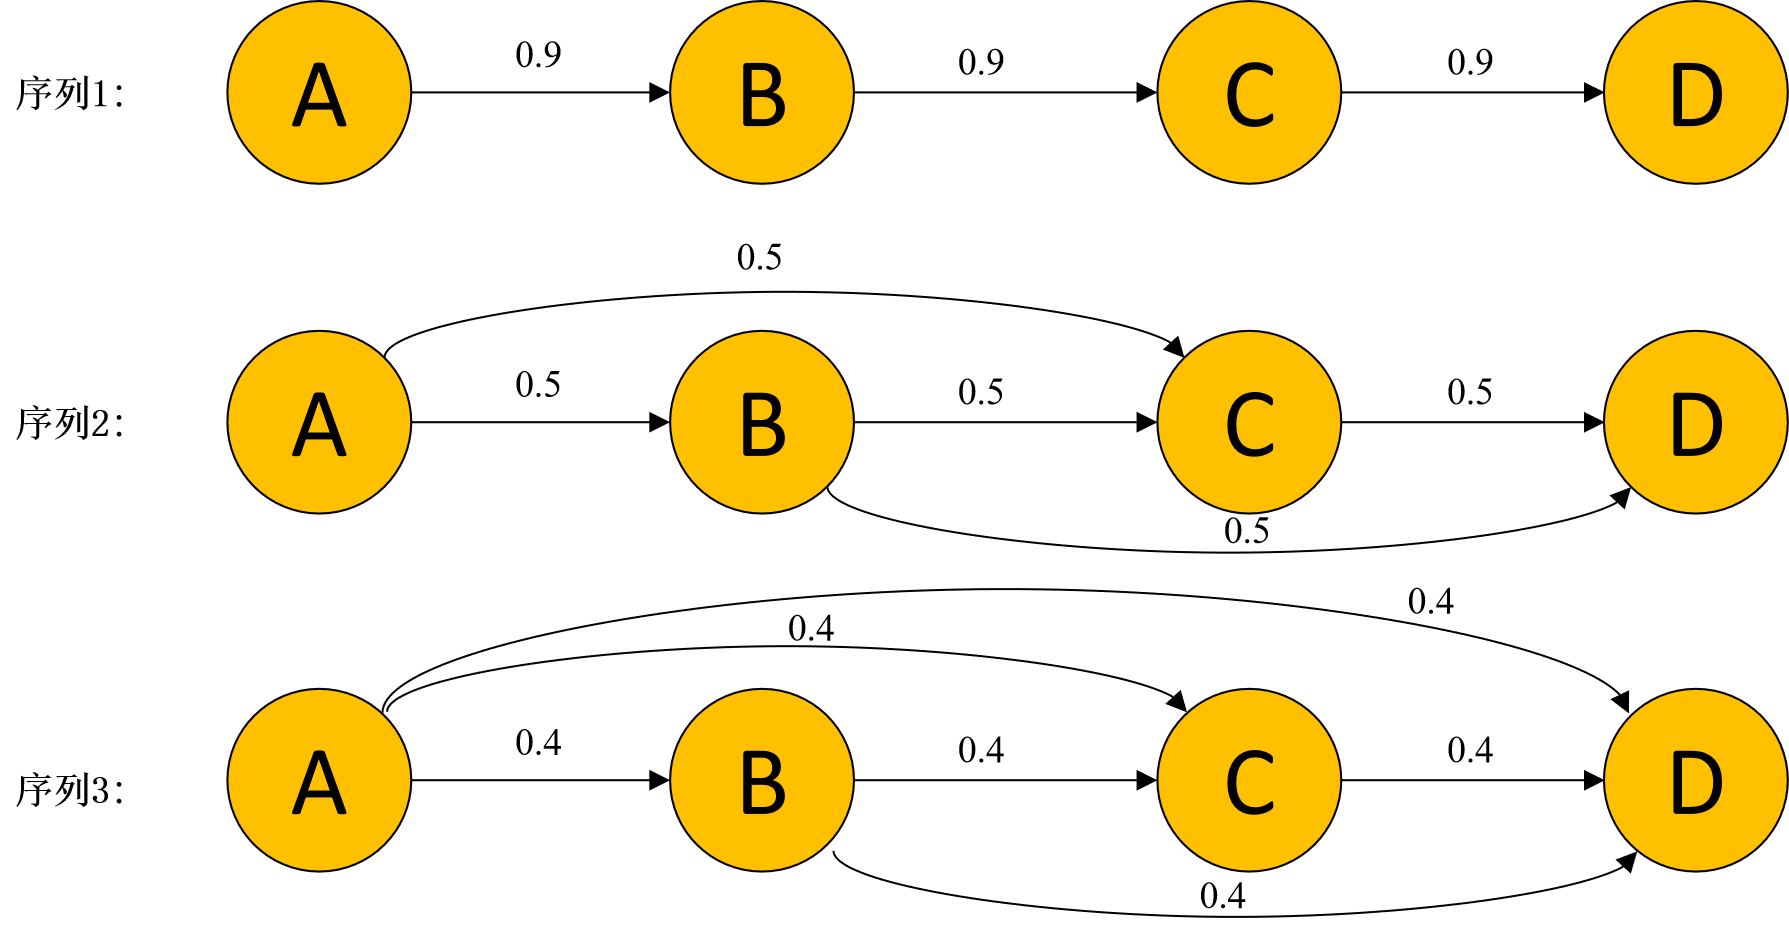
\includegraphics[width=.89\linewidth]{figure/rosenets/sample1}
    \caption{鲁棒网络子模序列示例}
    \label{fig:robust_sample}
\end{figure}

图\ref{fig:robust_sample}展示了三个具有不同鲁棒性的序列。在序列1中,所有边的权重均为0.9;序列2中,所有边的权重为0.5;而序列3中,所有边的权重为0.4。我们定义序列的网络子模函数$f$为序列生成边集的权重之和。这样定义的函数在生成点集上显然是单调的,但不具备子模性;然而,在边集上则具有子模性。通过计算可得,三个序列的整体价值分别为2.7(序列1,最大)、2.5(序列2)和2.4(序列3)。进一步分析发现,当从每个序列中移除一个节点时,序列1、2和3的最小价值分别为0.9、1.0(最大)和0.8。若移除两个节点,则序列1、2和3的价值分别变为0、0和0.4(最大)。

这一现象表明,随着移除节点数量的变化,三个序列表现出不同程度的鲁棒性性。传统的序列贪心算法\cite{tschiatschek2017selecting,mitrovic2018submodularity}可能会选择序列1,因为它具有最大的初始价值。然而,从鲁棒性的角度来看,序列2和序列3对节点移除表现出更强的鲁棒性。已有不少研究关注于集合子模函数的鲁棒性工作\cite{orlin2018robust,bogunovic2017robust,mitrovic2017streaming,tzoumas2017resilient},但关于序列网络子模函数鲁棒性的研究仍存在明显空白。针对这一问题,本文提出了鲁棒序列网络子模最大化算法。该算法不仅填补了理论研究的空白,还为序列广告推荐等实际应用提供了新的解决方案。我们的算法在保持序列网络子模函数优势的同时,引入了鲁棒性考虑,使得推荐结果在面对最差情况时能够表现出更好的鲁棒性和可靠性。

在社交网络的背景下,我们注意到用户并非孤立存在,信息会在用户的社交网络中不断传播,产生更广泛的影响。这种现象在各种平台上都有体现:在淘宝、Amazon等交易平台中,用户可以通过商品评价相互交流,分享对商品的看法。而在Twitter、Facebook(国外)和微博、微信(国内)等专门的社交平台上,拥有大量粉丝的博主只需发布一条信息,就可能促成大量交易。社交网络已经渗透到我们的网络生活的方方面面。正因如此,信息可以通过"口碑效应"在社交网络中迅速传播,产生巨大的影响力。这种社交网络中的信息传播过程吸引了多个领域的广泛研究,包括计算机科学、物理学、流行病学等\cite{li2018influence}。

社交网络影响力最大化问题(Influence Maximization问题,简称IM问题)最早由Richardson和Domingos等人\cite{richardson2002mining}在2002年提出,主要用来研究“口碑效应(Word-of-Mouth)”和“病毒营销(Viral marketing)”,后由Kemp等人\cite{kempe2003maximizing}模型化为算法问题,即在用户网络中选取一个种子集合,向他们投放广告,通过网络传播,最大化受影响的用户数量。Kempe等人引入了后来广泛使用的独立级联模型\cite{goldenberg2001talk}和线性阈值模型\cite{granovetter1978threshold},还提出了触发模型(Triggering Model,简称TR模型),证明了影响力最大化问题在这三种模型上都是NP-hard的,并给出了近似比为$1-1/e$的贪心算法。贪心算法在估算节点的边际收益时需进行大量蒙特卡洛模拟过程,时间复杂度较高,后续的工作大多针对这一点进行优化。

Borgs等人\cite{borgs2014maximizing}提出的反向影响力采样(Reverse Influence Sampling,简称RIS)技术在这一点上做出了突破性的贡献。该方法给出相同的近似比$1-1/e-\varepsilon$,时间复杂度仅为$O(k(m+n)log^2n/\varepsilon^2)$。基于这一思路,Tang等人相继提出了TIM/TIM+\cite{tang2014influence}和IMM\cite{tang2015influence}算法,运用鞅论方法,对时间复杂度进行了优化,达到了更低的了$O(k(m+n)logn/\varepsilon^2)$。Sun等人关注实际应用场景,建模了多轮影响力传播模型并提出了多轮影响力最大化问题\cite{mrim}。尽管影响力最大化领域的研究众多,但大多数研究默认用户都会接受推荐的广告,也不会考虑广告推荐顺序的不同影响。

应对这一问题,Tang\cite{tang2018social}首次将社交广告序列推荐和影响力最大化问题结合起来,假定用户逐个按顺序到来,为每一个到来的用户都推荐一组序列广告,用户根据兴趣概率接受部分广告,并有可能停止浏览。该研究将广告按照用户在网络上传播的期望收益与用户放弃继续浏览的概率比值进行排序,然后利用动态规划算法选择最终的广告序列,综合考虑了用户兴趣和网络传播效果。然而,这项研究仍然忽略了广告之间的关联,未考虑到用户对广告的接受程度很可能受其他广告的影响。

本文在广告序列推荐问题上首次将广告网络和用户网络同时纳入模型,在已有的影响力最大化问题和广告推荐问题的基础上,综合用户对广告的偏好、广告之间的促进作用以及用户网络的信息传递,并考虑到广告推荐不是一次性过程,加入多轮推荐的模式,建立能够同时为一组用户服务的多轮广告序列影响力最大化问题模型。并给出了基于多轮反向影响力采样方法和三明治方法的边贪心算法,为广告序列推荐提供了新的解决方案。

\section{研究内容}

本文在现有研究的基础上,针对以下三个问题做出改进:
(1) 现有的研究大多更关注用户对广告本身的兴趣,广告与广告之间的正向促进作用往往被忽略。
(2)用户可能不接受部分广告,这部分广告可能引起序列整体价值较大的变化。
(3)在社交网络日渐发达的背景下,用户并非孤立,用户接受广告的行为也会进一步影响到其他的用户,也需要考虑每个用户在社交网络中的信息传播作用。

针对上述问题的第一点和第二点,我们提出了鲁棒序列网络子模最大化算法。这部分工作的贡献主要体现在以下几点:(1)将网络子模性质引入广告序列推荐问题。网络子模性质的特点在于序列函数可以等价转化为关于边集的函数。这类函数对于序列的生成边集具有子模性,对于生成点集不一定具有子模性。使用这样的函数作为目标函数,可以使函数在最大化的过程中更加注重广告与广告之间的正向关联。(2)为广告序列推荐加入了鲁棒性考虑,用户可能会选择性不接受部分广告。本文提出了鲁棒序列网络子模最大化问题,最多为用户推荐长度为$k$的序列广告。考虑最差情况下,移除$\tau$个节点,序列剩余价值的最大化。(3)已有的序列贪心算法\cite{tschiatschek2017selecting,mitrovic2018submodularity}选出的序列,其价值往往集中于少数中心节点。只要移除这部分节点即可极大地破坏序列的价值。因此本文提出的鲁棒序列网络子模最大化算法采用两段式推荐,避免序列价值过度集中,从而提升广告序列的鲁棒性。
(4)证明并分析了鲁棒序列网络子模最大化算法的近似性。通过三个引理分别证明了算法在$\tau = 1$ 和$1< \tau < k$时的近似比。
(5)通过Amazon评论数据集上\cite{ni2019justifying}上的广告推荐实验和Wikispeedia数据集\cite{west2009wikispeedia}上的链路预测实验证明了鲁棒序列网络子模最大化算法的有效性。

将鲁棒序列网络子模最大化的工作和社交网络影响力最大化结合起来,我们提出了多轮社交广告序列影响最大化问题。这部分工作的贡献主要体现在以下几点:(1)创造性地将广告网络和用户社交网络同时融入模型,综合用户对广告的偏好、广告之间的促进作用以及用户网络的信息传递,并考虑到广告推荐不是一次性过程,加入多轮推荐的模式,建立能够同时为一组用户服务的多轮广告序列影响力最大化问题模型。(2)详细定义了多轮广告序列影响力最大化问题目标函数的计算方法。与鲁棒序列网络子模最大化问题不同的是,由于加入了社交网络信息传播的因素,用户不接受广告的最差情况很难计算,因此对于序列的鲁棒性考虑采用期望的形式来考虑用户对广告的接受程度。(3)提出了基于边贪心的多轮社交广告序列影响最大化推荐算法,并分析了其近似比。(4)边贪心的过程中需要快速估算每一条边的边际收益,为此,本文提出了针对多轮社交广告序列影响最大化问题的多轮反向影响力采样方法。(5)对目标函数的网络子模性进行分析,发现目标函数在边集上并不满足子模性,使用三明治夹逼的方法解决这一问题。并分析了使用多轮反向影响力采样方法和三明治方法的的边贪心算法的近似比和时间复杂度。
(6)扩展了动态多轮社交广告序列影响最大化以适应动态可以观测推荐结果的场景。
(7)最后再Amazon评论数据集\cite{amazon24}上的商品推荐实验证明了多轮社交广告序列影响最大化推荐算法的有效性。

综上所述,本文的主要贡献体现在以下几点:

\begin{itemize}
\item 引入网络子模性质到广告序列推荐问题中,使用网络子模函数描述广告序列,以便算法在最大化目标函数时更加重视广告网络中的信息,充分利用广告之间的正向作用关系。
\item 结合鲁棒性考虑,提出了鲁棒序列网络子模最大化问题,并提供了两段式边贪心策略。这种策略为用户推荐的鲁棒广告序列在用户拒绝部分广告的最坏情况下仍能保持较高的序列价值。并且对算法的近似性和复杂性进行了分析。
\item 结合社交网络背景,将影响力最大化问题进一步引入广告序列推荐任务中。创造性地将广告网络和用户社交网络同时融入模型,综合用户对广告的偏好、广告之间的促进作用以及用户网络的信息传递,提出了多轮社交广告序列影响最大化问题,并给出了基于边贪心、多轮反向影响力采样方法和三明治方法的解决方案。拓展了动态多轮社交广告序列影响最大化问题。并对算法的近似性和复杂性进行了分析。
\item 在真实数据集上进行了对比试验,验证了本文提出方法的有效性。
\end{itemize}


\section{论文组织结构}

本文一共分为六个章节,每个章节的组织结构如下所示:

第一章为绪论。介绍了研究背景,并对序列广告推荐这一领域目前存在的主要问题和研究内容进行了阐述,最后介绍了本文的组织结构。

第二章为相关工作。介绍了网络广告推荐、鲁棒子模最大化问题和影响力最大化问题的相关工作。阐述了本文研究所涉及领域的研究现状。

第三章为鲁棒序列网络子模最大化。结合广告之间的正向作用和鲁棒性考虑,提出了鲁棒序列网络子模最大化问题,设计了相应的边贪心算法,并分析证明了其近似比和时间复杂度。

第四章为多轮社交广告序列影响最大化。结合影响力最大化的工作,提出了多轮社交广告序列影响最大化问题。设计了边贪心框架、解决快速估算边际收益问题的多轮反向影响力采样方法,解决目标函数不具备子模性的三明治方法,得到多轮社交广告序列影响最大化问题的合理解决方案,并分析了其近似比和复杂度。拓展了动态多轮社交广告序列影响最大化问题。

第五章为实验结果和分析。介绍了每个实验的设计细节、使用的数据集、参数设置等。展示了对比实验结果,验证并分析了本文提出的算法的优势。

第六章为总结与展望。对本文的研究方法和研究结果进行总结,并对未来工作进行了展望。

% \section{本章小结}
% 本章首先介绍了广告序列推荐的研究背景,梳理了目前工作所面临的问题,引出并介绍了本文研究内容。最后对本文的组织结构进行了阐述。


\chapter{相关工作}

\section{网络广告推荐}
\label{sec:2_1}

随着电子商务和互联网技术的迅速发展,有大量研究致力于网络广告这一主题。在网络广告的早期阶段,基于关键词的拍卖模式占据主导地位,研究重点主要集中在提高点击量上。Edelmand等人\cite{edelman2007internet}基于拍卖机制,关注广告位上不同广告的点击率以提升广告效率。Attenberg等人\cite{attenberg2009modeling}采用了更为先进的方法,通过分析用户点击后的行为模式来预测未来行为,从而优化点击率。

另一类研究通过机器学习的方法尽可能准确推送用户喜欢的商品来提高点击率\cite{Cai2021,li2021effective},需要通过对用户的个人画像进行分析,从商品库中匹配到最适合用户的商品。这类方法往往需要大量数据对模型进行训练。

随着社交媒体平台的兴起和普及,用户在这些平台上花费的时间显著增加,他们不仅浏览内容,也接触到大量广告,这一趋势促使广告投放方式发生了变化。Alaei等人\cite{alaei2021maximizing}的工作利用子模函数建模广告序列推荐问题,为用户推荐序列广告,实现了$1-1/e$的近似比。但该研究未考虑用户可能拒绝部分广告的情况。在实际应用中,用户的选择性和互动行为是不可忽视的因素,这直接影响广告的有效性和用户体验。

一部分研究,如Kempe等人\cite{kempe2008cascade}、Craswell等人\cite{craswell2008experimental}和Tang等人\cite{tang2017robust}的工作,考虑了用户行为的随机性。他们假定人与人之间是独立的,对于广告序列,他们会从上到下依次浏览,感兴趣的就点击链接购买或者了解相关信息,不喜欢的就略过,在浏览完一个广告后会有概率结束浏览,广告商会按照广告被点击的次数付给推荐平台广告费用。这些模型倾向于将更具吸引力的广告排在前面,以延长用户的浏览时间并最大化收益。这种方法更注重用户对广告的兴趣,但忽略了广告之间可能存在的协同效应。

尽管这些研究考虑了广告顺序对序列效果的影响,但它们未能充分捕捉广告之间的正向促进关系。为了弥补这一研究空白,本文引入了网络子模序列函数来描述广告序列的价值。这一方法能够综合考虑用户偏好和广告间的相互作用,为广告序列优化提供了更加全面和精确的理论框架。

\section{鲁棒子模最大化问题}
\label{sec:2_2}

\subsection{子模最大化问题和网络子模性}

子模性是一种描述边际收益递减现象的重要数学性质。在学术文献中,子模性已成为广泛研究的主题,尤其在集合函数的最大化或最小化问题中经常发挥关键作用\cite{nemhauser1978best,khuller1999budgeted}。这一概念源于现实中常见的现象:随着集合规模的扩大,向其中添加新元素所带来的边际价值通常会逐渐减少。从数学角度定义,如果对于任意两个集合$A\subseteq B \subseteq V$和一个元素$v\in V\backslash B$,集合函数$f: 2^V \to \mathbb{R}$满足$f(A\cup v) - f(A) \ge f(B\cup v) -f(B)$,则该函数是子模的。这种性质在机器学习、组合优化、经济学等领域都有广泛的应用\cite{krause2005near,lin2011class,shi2021profit,kirchhoff2014submodularity,gabillon2013adaptive,kempe2003maximizing,wang2021efficient}。

将子模函数结合单调性,进一步为解决优化问题提供强大的理论基础。单调性是指,对于任意$A\subseteq B\subseteq V$,有$f(A)\le f(B)$。在有集合带下限制的约束下,单调子模集合函数的最大化问题可以通过经典的贪心算法得到有效解决。这种方法能够达到$1−1/e$的近似比\cite{nemhauser1978best},这几乎是理论上可能达到的最佳结果。自此之后,对子模函数的研究已经扩展到考虑各种不同的场景,如非单调场景、自适应场景和连续场景等\cite{feige2007maximizing,golovin2011adaptive,das2011submodular,bach2019submodular,shi2019adaptive}。

上述研究主要聚焦于集合函数,但实际应用中的许多问题往往更为复杂。尤其是元素被添加的顺序在很多场景下非常重要,并可能对目标函数值或实际效果产生很大的影响。近年来,子模性已经被推广到序列函数\cite{zhang2015string,tschiatschek2017selecting,streeter2008online,zhang2013near}。从集合到序列的拓展会导致搜索空间和计算复杂性呈指数级增长,对于一个包含$n$个元素的集合,其所有可能的排列数量为$n!$,远远超过$2^n$个子集的数量。但同时也可以极大的增强模型的表达能力,序列模型能够捕捉元素间的顺序关系,能够处理更加复杂和细致的优化任务。

Tschiatschek等人\cite{tschiatschek2017selecting}和Mitrovic等人\cite{mitrovic2018submodularity}工作中的序列函数最大化设定其中元素通过有向图进行连接,图中的边表示当前相连的元素以特定顺序被选择时产生的额外价值。这种设定的特殊之处在于,这种函数是一个关于序列的函数,而非关于元素集合的函数。它在序列的生成元素集合上可以是非子模的,而需要在序列的生成边集上满足子模性。由于这种函数性质之前并没有命名,在本文中,我们暂且将其称之为网络子模性。Tschiatschek等人\cite{tschiatschek2017selecting}首次考虑最大化网络子模函数,Mitrovic等人\cite{mitrovic2018submodularity}还考虑到了超图上的情况。

\subsection{鲁棒子模最大化问题}

近年来,随着实际应用中对系统稳定性和可靠性要求的提高,鲁棒子模最大化问题也得到了广泛研究。这类问题的核心在于选择一组元素,使得即便在部分元素被移除的情况下,结果仍能保持良好的性能。这种鲁棒性考虑反映了现实世界中不可避免的不确定性。

在这一领域的开创性工作中,Orlin等人\cite{orlin2018robust}首次系统研究了具有集合大小限制下的鲁棒子模最大化问题。他们提出的算法能够在常数近似比的保证下,选择$k$个元素的集合,使其对任意$\tau$个元素的移除具有鲁棒性。这一结果在$\tau = O(\sqrt{k})$的条件下有效,为后续研究奠定了基础。

随后,Bogunovic等人\cite{bogunovic2017robust}在此基础上进行了显著改进。他们提出的算法不仅保持了常数近似比的保证,还将可移除元素的数量扩大到$\tau = O(k)$,大大增强了算法的实用性和鲁棒性。

在一个更为宽松的假设条件下,Mitrovic等人\cite{mitrovic2017streaming}进一步推进了研究边界,提出了一种允许移除任意数量元素的算法。这一突破性成果极大地提高了算法在面对大规模故障或攻击时的适应能力。

Tzoumas等人的工作\cite{tzoumas2017resilient}则采取了不同的方向,他们放宽了对$\tau$的限制,但得到的近似比与$\tau$相关。这种权衡为不同应用场景提供了更灵活的选择。该研究随后在\cite{tzoumas2018resilient}和\cite{tzoumas2020robust}中被扩展到多阶段设置,使算法能够在每个决策阶段考虑前几个阶段发生的故障,从而实现动态的鲁棒优化。

除了基本的鲁棒性考虑,研究者们还探索了将鲁棒优化与其他重要约束相结合的可能性。例如,Mirzasoleiman等人\cite{mirzasoleiman2017deletion}和Kazemi等人\cite{kazemi2018scalable}的工作考虑了公平性和隐私保护等因素,进一步拓展了鲁棒子模最大化的应用范围。但关于序列网络子模函数鲁棒性的研究仍存在明显空白。


\section{影响力最大化问题}
\label{sec:2_3}

随着移动设备的普及和信息网络的飞速发展,人们上网越来越便利,在社交网络中的沟通交流因打破了时间和空间的限制而备受欢迎。社交网络影响力最大化问题最早由Richardson和Domingos等人\cite{richardson2002mining}在2002年提出,主要用来研究“口碑效应(Word-of-Mouth)”和“病毒营销(Viral marketing)”。“病毒营销”是指商家在宣传产品时,找到人群中影响力较大的人,用请他们免费试用等形式,通过他们的影响力和口碑效应,让更多的人了解并认可这一产品,以获得更大的经济效益。病毒营销的方法在社交网络兴起的时代应用起来更为便利,例如许多商家会找社交网络中拥有众多粉丝的博主合作宣传产品,相比于商家直接投放在平台上的广告,粉丝们更愿意相信他们关注的博主,他们对产品的印象和感受又会通过社交网络传递给他们的朋友,如此循环往复,影响力的传播就像病毒一样不断在网络上扩散。利用社交网络上的信息传播,商家可以用更小的广告成本,换取更大的知名度,这也是社交广告相较于传统营销广告的优点。后来,影响力最大化问题还被广泛应用在广告投放\cite{zhang2020geodemographic,zeng2021business,saleem2019effective}、谣言抑
制\cite{shi2019adaptive,zhong2023rumor,myilsamy2024optimal}、链路预测\cite{tripathi2022network,daud2020applications}等领域。


\subsection{影响力传播模型}

Domingos和Richardson等人\cite{domingos2001mining}提出了基于马尔科夫随机场(Markov Random Field)的社交网络影响力模型,建模了节点之间影响力被激活的相关性。社交网络被抽象为一个有向图$G(V,E)$,节点代表用户,每个节点分为两种状态:激活(active)状态和未激活(inactive)状态,节点被激活可以被视为信息传播到了该用户,但该模型并没有体现出节点之间影响力传播的关系。后来Kempe等人\cite{kempe2003maximizing}引入了更加符合人们直觉的独立级联(Independent Cascade)模型,线性阈值模型(Linear Threshold)模型和触发模型(Triggering)。结合更多实际情况,研究人员还提出了时间感知模型\cite{chen2012time}和疾病传播模型\cite{shah2010detecting}等。接下来介绍几种常用的影响力传播模型。

独立级联模型是使用最为广泛的影响力传播模型,该模型假设用户与用户之间的影响力传播是相互独立的,对于社交网络$G=(V,E)$中的每一条边$e=(u,v)$,都关联一个影响力概率$p_{u,v}$。初始情况下所有节点均处于未激活状态。该模型的传播过程定义在若干离散的时刻上,从$t=0$时刻开始。给定一个种子节点集合$S$,当时刻$t=0$时,种子集合$S$中的全部节点均被激活。当时刻$t \ge 1$时,每一个已被激活的节点$u$都会尝试激活在$t-1$时刻还未被激活的出边邻居$v$,有$p_{u,v}$的概率成功,如果成功则$v$会被激活,否则$v$保持原状态不变。需要注意的是,无论是否激活成功,$u$都会保持激活状态并停止激活动作,即$u$在以后的任意时刻都不会再尝试激活它的出边邻居。当没有任何新节点被激活时,传播过程结束。因其准确简洁的传播模式,大部分主流的社交网络影响力传播的工作都采用了独立级联模型。

线性阈值模型由Granovetter和Schelling在1978年首次提出\cite{granovetter1978threshold}。在线性阈值模型中,对于社交网络$G=(V,E)$中的每一条边$e=(u,v)$,都关联一个权重$b_{u,v}$,该权重分配需要满足$\sum_{u \in \mathcal{N}(v)}b_{u,v}\le1$,其中$\mathcal{N}(v)$代表$v$的入点集合,每个用户节点$v$还会有一个阈值$\theta_v \in [0,1]$。和IC模型相同,该模型的传播步骤也是在离散的时刻上进行。给定种子集合$S$,在$t=0$时刻,$S$中的所有节点均被激活。在$t\ge1$的时刻,所有在$t-1$时刻已被激活的节点仍然保持激活状态,未被激活的节点$v$会计算并判断是否$\sum_{u \in \mathcal{N}(v);u \ is \ active} b_{u,v} \ge \theta_v$,即在所有$v$的入点中,如果被激活的节点的总权重不低于阈值$\theta_v$,则节点$v$将会在该时刻变为激活状态,反之则保持未激活状态。传播直到没有任何新增激活节点时结束。相比于独立级联模型,线性阈值模型兼顾了多条传播之间的效果累加和用户节点本身的接受程度,能够表达出的含义更加的丰富,但是在阈值的选择上会增大模型的分析和计算难度\cite{chen2013information}。

本文使用到的触发模型(Triggering Model)是一种更加通用的模型。同样地,在$t=0$时刻,种子集合$S$中的所有节点均被激活,并且会对每一个$V$中节点$v$独立随机地根据其入边关联的概率生成一个触发集合$T(v)$,$T(v)$是$v$的入边邻居集合的一个子集。当$t\ge 1$时,对于每个未被激活的节点$v$,如果在$t-1$时刻,$T(v)$中有至少一个节点已经被激活,那么节点$v$将会在$t$时刻被激活。传播直到没有任何新增节点时结束。由于独立级联模型和线性阈值模型更容易对应到具体的可解释场景中,在研究过程中往往会延伸出更多这两种模型的变种模型,因此应用较为广泛。但触发模型能够概扩另外两种模型,独立级联模型和线性阈值模型被证明都是它的一种特例\cite{kempe2003maximizing}。


\subsection{影响力最大化算法}

Kempe等人\cite{kempe2003maximizing}于2003年首次对社交网络影响力最大化问题进行了形式化定义。该问题可描述如下:给定一个社交网络$G=(V,E)$和一个正整数$k$,其中$V$表示社交网络中的用户集合,$E \subseteq V \times V$代表用户之间的关系边。影响力最大化问题的目标是找到一个大小不超过$k$的用户子集$S^*$,使得该子集中的用户能在整个社交网络中产生最大的影响力。

Kempe等人证明了在独立级联模型、线性阈值模型以及触发模型下,影响力最大化问题均为NP-hard。然而,他们同时证明了这些模型都满足子模性质,这一特性保证了贪心算法能够达到$1-1/e-\varepsilon$的近似比。该贪心算法的具体步骤如下:
1. 初始化种子集合为空集;
2. 在每一轮迭代中,选择能够带来最大边际收益的节点,将其加入种子集合;
3. 重复步骤2,直到种子集合的大小达到预设的$k$值。

虽然贪心算法可以得到较好的近似比,但是对每个节点计算其边际收益仍是一个具有挑战性的问题。Kempe等人使用了比较直观的蒙特卡洛模拟(Monte Carlo Simulation)方法,即进行多次模拟传播,最终取平均值作为真值的无偏估计。这种方法的缺点在于复杂度太高,算法要重复$k$轮,计算边际收益需要遍历$n$个点,为了保证估计值的准确性,需要$R$次模拟,每次模拟都要遍历$m$条边,时间复杂度$O(knmR)$,耗时巨大。真实的社交网络规模庞大,这样的方法很难得以实际应用,因此研究者针对提升模拟效率进行了许多研究。

Leskovec等人提出了CELF(Cost-Effective Lazy Forward)算法\cite{leskovec2007cost}。CELF利用了影响力最大化问题的子模性,减少了计算节点边际收益的次数,从而降低了算法的复杂度。它的优化原理是:如果一轮中如果某个节点上一轮的边际收益小于其他任意节点本轮的边际收益,那么根据边际收益递减,就不必对该节点再次计算。CELF优化大幅提升了算法效率,运行速度提高了700倍。Goyal等人\cite{goyal2011celf++}在此基础上又提出了CELF++算法,通过对边际收益增加标记的方法再次提升了运行效率。还有许多工作在模拟方法的基础上持续优化其运行效率\cite{kumar2022csr,王璿2022基于社交网络的影响力最大化算法},但是在大规模的图上这类算法仍然需要耗费大量时间。另一个研究方向是启发式算法,利用传播模型的某些特性来提高特定情况下的算法效率\cite{kumar2022mder,lozano2024efficient,chen2009efficient,chen2010scalable,chen2010scalable2,goyal2011simpath},启发式算法的运行速度提升很大,但是并没有近似比的保证。

Borgs等人\cite{borgs2014maximizing}提出的反向影响力采样(Reverse Influence Sampling,简称RIS)技术做出了突破性的贡献。反向影响力采样是指先随机选一个点,从该节点反向模拟,也就是找到哪些节点作为种子节点时能影响到该节点,这些节点的集合被称为反向可达集合(Reverse Reachable set,简称RR set)。基于RIS的影响力最大化算法先收集足够多的RR set,然后通过贪心找到一个能够覆盖尽可能多的RR set的种子节点集合。该算法给出了相同的近似比$1-1/e-\varepsilon$,时间复杂度仅为$O(k(m+n)log^2n/\varepsilon^2)$。基于这一思路,Tang等人相继提出了TIM/TIM+\cite{tang2014influence}和IMM\cite{tang2015influence}算法,运用鞅论的分析方法,对时间复杂度进行了优化,达到了$O(k(m+n)logn/\varepsilon^2)$。IMM算法的出现使得影响力最大化算法在近似比得到保证的情况下,在庞大的社交网络中也能够具有良好的实用性。

Sun等人关注实际应用场景,建模了多轮影响力传播模型并提出了多轮影响力最大化问题(Multi-Round Influence Maximization,简称MRIM问题)\parencite{sun2018multi},将影响力最大化问题扩充为$T$轮传播,每轮选择最多$k$个节点的种子集合,使得传播结束时被激活的节点尽可能多。Sun等人提出了静态和动态两种基于IMM的多轮贪心算法,均能保证$1-e^{-(1-1/e)}-\varepsilon$的近似比。Lozano-Osorio等人\cite{lozano2022multi}在此基础上提出智能邻域搜索策略进一步提高了多轮影响力最大化问题可扩展性。


\subsection{影响力最大化在广告推荐中的应用}

影响力最大化在广告推荐领域的一个重要方向是地缘推荐\cite{zhang2020geodemographic,zeng2021business,saleem2019effective}。这类方法利用人口分布、移动统计数据以及社交网络中的位置影响力,旨在确定最佳的广告投放位置或影响力最大化策略。通过引入影响扩散模型和位置影响概念等模型和算法,这些方法能够有效选择广告投放位置,从而最大化预期覆盖范围或影响力,提升广告效果和社交网络营销的效率。Li等人\cite{li2015real}关注目标感知,考虑用户是否能有效促进信息传播,通过实时从社交网络中找到最有影响力的用户来推荐项目。Cor{'o}等人\cite{coro2021link}提出了一种基于用户社会影响力的链接推荐算法,通过评估链接的社会影响力增量来推荐链接,以最大化目标用户的社会影响力。

影响力最大户算法在广告推荐领域中的绝大部分研究都旨在对特定的广告,找到影响力最大的用户,通过给这部分高影响人群推荐广告而达到利益最大化,而较少考虑那些非高影响用户。且大多都默认用户一定会接受推荐给他们的广告,也不会考虑广告推荐顺序的差异。

为了解决这一挑战,Tang\cite{tang2018social}首次将社交广告序列推荐和影响力最大化问题结合起来,假定用户逐个按顺序到来,为每一个到来的用户都推荐一组序列广告,用户会根据自身兴趣概率接受部分广告,并有可能停止浏览。该研究将广告按照用户在网络上传播的期望收益与用户停止浏览概率的比值进行排序,然后利用动态规划算法选择最终的广告序列,综合考虑了用户兴趣和网络传播带来的影响力。

\section{本章小结}

在本章中,主要介绍了本文相关领域的研究和技术。\ref{sec:2_1}介绍了网络广告推荐应用的相关工作及其发展。\ref{sec:2_2}介绍了子模性在序列选择领域的重要意义,以及子模最大化问题与鲁棒性结合的研究工作。\ref{sec:2_3}介绍了影响力最大化问题的发展,包括传播模型的种类、影响力最大化算法及其相关技术以及影响力最大化算法在广告推荐中的应用。



\chapter{鲁棒序列网络子模最大化}

\section{鲁棒序列网络子模最大化问题定义}
\label{sec:3_1}
在本文中,我们遵循Tschiatschek等人\cite{tschiatschek2017selecting}的设定。令$V={v_1,v_2,...,v_n}$代表$n$个广告节点的集合。一组边\(W\)表示按特定顺序选择某些广告节点会带来额外收益。更具体地,边\(e_{ij} = (v_i,v_j)\)表示在选择\(v_i\)之后选择\(v_j\)会带来额外收益。自环(即起始和结束于同一节点的边)表示选择一个节点本身会带来的收益。

\begin{definition}
{\bfseries 序列子模最大化问题}是指,给定一个有向图\(N = (V,W)\),一个非负单调子模集合函数\(h: 2^W \rightarrow \mathbb{R}_{\ge 0}\),和序列长度限制\(k\),目标是选择一个不重复的长度为\(k\)的节点序列\(\sigma\),使目标函数最大化:
\begin{equation}
    f(\sigma)=h(E(\sigma))
\end{equation}
\noindent 其中,\(E(\sigma)\) 为序列$\sigma$的生成边集,包含所有满足\((v_i,v_j)\in W\)且在\(\sigma\)中\(v_i\)出现在\(v_j\)之前的边。
\end{definition}

需要注意的是,函数\(h\)是关于边集的子模函数,而非节点集合。而目标函数\(f\)既不是一个集合函数,关于节点也不一定是子模的,但对于序列的生成边集满足子模性。我们将这样的函数\(f(\sigma)\)称为{\bfseries 网络子模}函数。

定义\(f(\sigma - Z)\)为$\sigma$在移除集合\(Z\)中的节点后目标函数的剩余价值。
\begin{definition}
{\bfseries 鲁棒序列网络子模最大化问题}是指,给定一个有向图\(G=(V,E)\)、一个网络子模函数\(f(\cdot)\)、序列长度限制$k$和鲁棒性参数\(\tau\),找到一个序列\(\sigma\),使其对最坏情况下移除\(\tau\)个节点仍具有鲁棒性:
\begin{equation}
    \max_{\sigma:|\sigma|\le k} \min_{Z\in \sigma,|Z|\le \tau} f(\sigma - Z)
\end{equation}
\end{definition}

鲁棒参数\(\tau\)表示被移除的子集\(Z\)的大小。在移除之后,目标值应尽可能保持大。当\(\tau = 0\)时,该问题简化为经典的序列子模最大化问题\cite{mitrovic2018submodularity}。

\section{鲁棒序列网络子模最大化算法}
\label{sec:3_2}

已有的序列贪心算法\cite{mitrovic2018submodularity}不会考虑节点被删除的情况,直接应用其来解决鲁棒序列网络子模最大化问题效果可能会比较糟糕。我们可以构造一个非常简单的例子来进行说明,如图\ref{fig:rose_sample}所示,边$(A,B),(B,C),(B,E),(B,F)$的权重为0.9,边$(C,D),(C,G),(D,G)$的权重为0.5。假设目标网络子模函数\(f\)是所选序列生成边集中所有边的权重总和,要选择一个包含5个节点的序列,使用序列贪心算法,为了最大化总价值,包含更多高权重边的序列\(\langle A,B,C,E,F \rangle\)将会被选中,价值为\((0.9 \times 4 = 3.6)\)。然而,如果设置\(\tau=2\),即移除两个节点,在最坏情况下,只要移除\(B\)和任意一个其他节点,都会使价值减为$0$。

\begin{figure}[th]
    \centering
    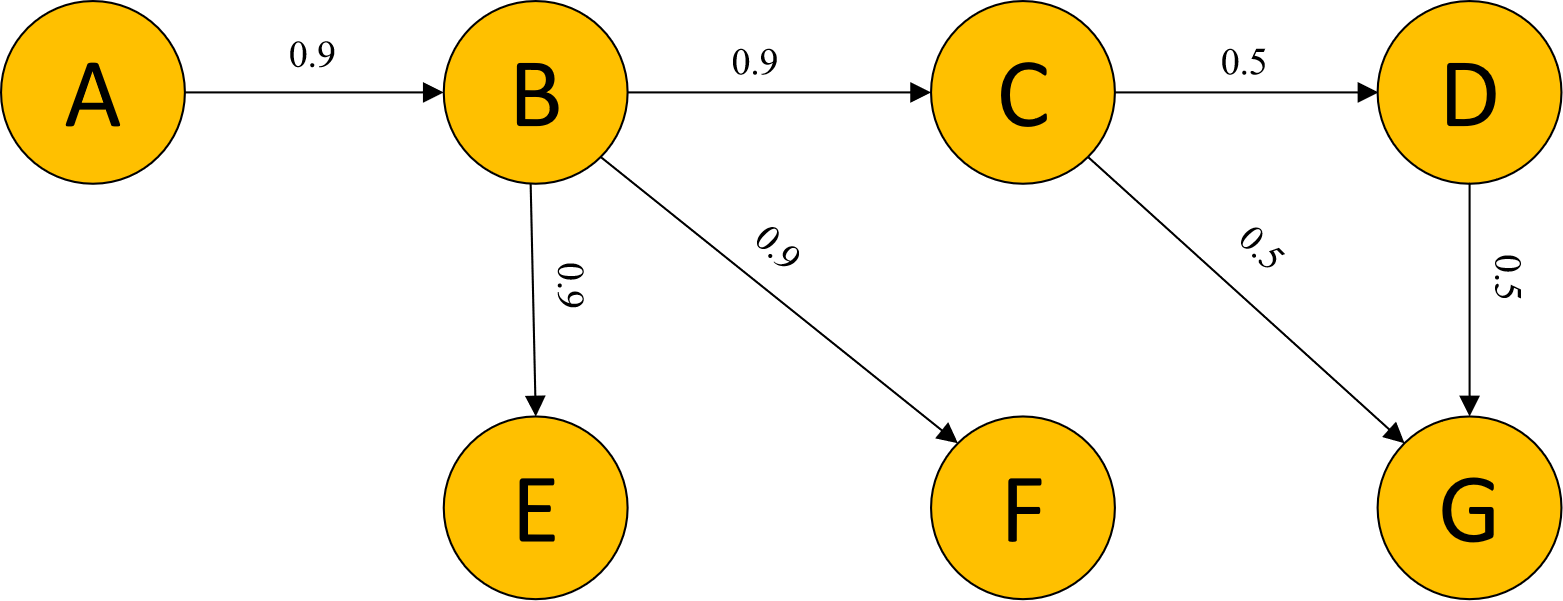
\includegraphics[width=.89\linewidth]{figure/rosenets/sample2}
    \caption{序列子模最大化示例}
    \label{fig:rose_sample}
\end{figure}

因此,我们希望设计一个在移除任意$\tau$个已选定节点时仍能保持鲁棒性的算法。我们提出了鲁棒序列网络子模最大化算法,该算法可以近似解决鲁棒序列网络子模最大化问题,如算法\ref{alg:rosenets}所示。考虑到最终的结果需要移除部分节点,我们仅考虑$k \ge 3$的情况。

序列贪心算法的局限性在于所选序列的整体价值可能集中在前几个节点上,导致个别节点被删除时对整体价值影响巨大。基于这一观察,算法\ref{alg:rosenets}分为两个步骤:第一步(第一个\textit{while}循环,第\ref{alg:rose_line1}到\ref{alg:rose_line2}行)中,我们以类似于序列贪心的方法从\(V\)中选择一个包含\(\tau\)个节点的序列\(\sigma_1\)。其中$h(e_{ij}|E(\sigma_1))=h(E(\sigma_1)\cup\{e_{ij}\})-h(E(\sigma_1))$,为边$e_{ij}$的边际收益。$\oplus$符号代表将两个序列顺序连接。第二步(第二个\textit{while}循环,第\ref{alg:rose_line3}到\ref{alg:rose_line4}行)中,以类似于序列贪心的方法从\(V\backslash \sigma_1\)中选择包含\(k-\tau\)个节点的另一个序列\(\sigma_2\)。需要注意的是,当我们选择序列\(\sigma_2\)时,我们会假定序列\(\sigma_1\)根本不存在,这确保了最终返回的序列\(\sigma = \sigma_1 \oplus \sigma_2\) 的价值不会集中在\(\sigma_1\)或\(\sigma_2\)中。算法\ref{alg:rosenets}的复杂度为\(O(k|E|)\),为算法中评估函数$h$值的次数。

\begin{algorithm}[H]
    \caption{鲁棒序列网络子模最大化算法 \label{alg:rosenets}}
    \begin{algorithmic}[1]
        \REQUIRE 有向图\(N = (V,W)\);非负单调子模集合函数\(h: 2^W \rightarrow \mathbb{R}_{\ge 0}\);参数$k, \tau$
        \ENSURE $\sigma$
        \STATE $\sigma_0=\emptyset$, $\sigma_1=\emptyset$, $\sigma_2=\emptyset$\;
        \WHILE{$|\sigma_1| < \tau$} \label{alg:rose_line1}
            \IF{$|\sigma_1|=\tau-1$}
                \STATE$e_{ij}=\arg\max_{\{e_{ij}|(v_i=v_j \text{ or } v_i \in \sigma_1) \text{ and } v_j\notin \sigma_1\}} h(e_{ij}|E(\sigma_1))$\;
                \STATE$\sigma_1 = \sigma_1 \oplus v_j$\;
            \ELSE
                \STATE $e_{ij}=\arg\max_{\{e_{ij}|v_j\notin \sigma_1\}} h(e_{ij}|E(\sigma_1))$\;
                \IF{$v_j=v_i$ or $v_i\in \sigma_1$}
                    \STATE $\sigma_1 = \sigma_1 \oplus v_j$\;
                \ELSE
                    \STATE $\sigma_1 = \sigma_1 \oplus v_i \oplus v_j$\;
                \ENDIF
            \ENDIF
        \ENDWHILE \label{alg:rose_line2}
        \WHILE{$|\sigma_2| < k-\tau$} \label{alg:rose_line3}
            \IF{$|\sigma_2|=k-\tau-1$}
                \STATE $e_{ij}=\arg\max_{\{e_{ij}|(v_i=v_j \text{ or } v_i \in \sigma_1 \cup \sigma_2) \text{ and } v_j \notin \sigma_1 \cup \sigma_2\}} h(e_{ij}|E(\sigma_2))$\;
                \STATE $\sigma_2 = \sigma_2 \oplus v_j$\;
            \ELSE
                \STATE $e_{ij}=\arg\max_{\{e_{ij}|v_i\notin \sigma_1, v_j \notin \sigma_1 \cup \sigma_2\}} h(e_{ij}|E(\sigma_2))$\;
                \IF{$v_j=v_i$ or $v_i\in \sigma_2$}
                    \STATE$\sigma_2 = \sigma_2 \oplus v_j$\;
                \ELSE
                    \STATE $\sigma_2 = \sigma_2 \oplus v_i \oplus v_j$\;
                \ENDIF
            \ENDIF
        \ENDWHILE \label{alg:rose_line4}
        \STATE $\sigma=\sigma_1\oplus \sigma_2$\;
    \end{algorithmic}
\end{algorithm}

回到图\ref{fig:rose_sample}中的例子。当\(k=5\)且\(\tau=2\)时,鲁棒序列网络子模最大化算法将选择序列\(\sigma_1=\langle A,B \rangle\)和序列\(\sigma_2=\langle C,D,G \rangle\)。在选择\(\sigma_2\)时,算法不会考虑序列\(\sigma_1\)中的节点\(B\)。因此,节点\(E\)和\(F\)被视为对目标函数没有贡献。算法将返回序列\(\sigma=\langle A,B,C,D,G \rangle\)。移除\(\tau=2\)个节点的最坏情况是移除\(B\)和\(\{C,D,G\}\)中的任意一个节点。剩余价值为0.5。而序列贪心函数得到的结果最坏情况的剩余价值为0。这个例子展现了鲁棒序列网络子模最大化算法的差异与优势。

一个鲁棒的序列应具有复杂的网络结构,其价值不应集中于少数中心节点,而应来源于序列中所有节点之间的边。要选择这样的鲁棒序列,需要进行多次相互独立的贪心选择尝试。这种方法可以避免单一贪心选择可能导致的问题,即高概率选中中心节点及其高边权邻居(如图\ref{fig:rose_sample}中的节点$B$),从而使得移除这些节点导致整体价值急剧下降。本文通过两次独立的贪心选择来实现这一策略。理论上,增加贪心选择的次数可能会提高算法的近似比。然而,考虑到这是鲁棒序列网络子模最大化问题研究的初步阶段,且当前的理论分析已相当复杂,我们将多部分选择算法的设计及其近似比分析留作未来研究课题。

\section{近似性分析}
\label{sec:3_3}

令 $\alpha=2 d_{\text{in}}+1$,$\beta=1+d_{\text{in}}+d_{\text{out}}$,$\gamma=e^{\frac{k-3}{k-2}}$,$\eta=e^{\frac{k-2\tau-1}{k-\tau-1}}$。其中,$d_{\text{in}}$ 和 $d_{\text{out}}$ 分别是网络中节点的最大入度和出度。

为了方便,我们用 $f(v|\sigma)$ 和 $f(\sigma'|\sigma)$ 分别表示将 $v$ 和 $\sigma'$ 添加到序列 $\sigma$ 后的边际增益。用 $\sigma^*(V,k,\tau)$ 表示鲁棒序列网络子模最大化问题的最优解,其中 $V$ 是节点集,$k$ 是选择序列的长度,$\tau$ 是鲁棒参数。$g_\tau(\sigma)$ 表示从序列 $\sigma$ 中移除 $\tau$ 个节点后 $f(\sigma)$ 的最小值(即最差情况)。

\begin{theorem}
\label{thm:tau1}
当 $\tau=1$ 时,鲁棒序列网络子模最大化算法的近似比可以达到
\begin{equation}
\max\{\frac{1-e^{-(1-1/k)}}{\alpha\beta},\frac{\gamma^{\frac{1}{d_{\text{in}}}}-1}{\beta \gamma^{\frac{1}{d_{\text{in}}}}-1}\}\end{equation}
\end{theorem}

\begin{theorem}
\label{thm:tau2}
当 $1\le \tau \le k$时, 鲁棒序列网络子模最大化算法的近似比可以达到
\begin{equation}
 \max\{\frac{1-e^{-(1-1/k)}}{\alpha\beta},\frac{\tau\alpha\beta(\eta^{\frac{1}{d_{\text{in}}}}-1)}{\tau\alpha\eta^{\frac{1}{d_{\text{in}}}}- \beta (1-e^{-(1-1/k)}) }\}    
\end{equation}
\end{theorem}

在定理\ref{thm:tau1}中,由于两个近似比下限的数学表达式较为复杂,很难直接进行比较。因此,我们考虑特定的情况来展示这两项的大小关系。

首先,很容易验证这两项都是关于 $k$ 的单调递增函数。当 $k=3$ 时,我们有 $\frac{1-e^{-(1-1/k)}}{\alpha\beta}-\frac{\gamma^{\frac{1}{d_{\text{in}}}}-1}{\beta \gamma^{\frac{1}{d_{\text{in}}}}-1} = \frac{1-e^{-2/3}}{\alpha \beta}>0$。因此,我们知道当 $k$ 较小时,第一项更大。当 $k \to \infty$ 时,第一项的极限值为 $(1-1/e)/\alpha\beta$,第二项的极限值为 $\frac{e^{\frac{1}{d_{\text{in}}}}-1}{\beta e^{\frac{1}{d_{\text{in}}}}-1}$。当 $d_{\text{in}}=1$ 时,$\alpha=3$,且 $(1-1/e)/\alpha\beta-\frac{e^{\frac{1}{d_{\text{in}}}}-1}{\beta e^{\frac{1}{d_{\text{in}}}}-1} =(1-1/e)/3\beta-\frac{e-1}{\beta e-1}=\frac{-1-2\beta e +\frac{1}{e}+2\beta}{3\beta(\beta e-1)}<0$。在这种情况下,定理\ref{thm:tau1}中的第二项大于第一项。因此,我们可以得出,在特定的网络结构下以及 $k$ 较大时,第二项会更大。

类似地,对于定理\ref{thm:tau2},当 $k=3$ 且 $\tau=1$ 时,$\frac{1-e^{-(1-1/k)}}{\alpha\beta}-\frac{\tau\alpha\beta(\eta^{\frac{1}{d_{\text{in}}}}-1)}{\tau\alpha\eta^{\frac{1}{d_{\text{in}}}}- \beta (1-e^{-(1-1/k)})} = \frac{1-e^{-2/3}}{\alpha \beta}>0$。因此,我们知道当 $k$ 和 $\tau$ 较小时,第一项更大。当 $k \to \infty$ 而 $\tau$ 保持常数时,第一项的极限值为 $(1-1/e)/\alpha\beta$,第二项的极限值为 $\frac{\tau\alpha\beta(e^{\frac{1}{d_{\text{in}}}}-1)}{\tau\alpha e^{\frac{1}{d_{\text{in}}}}- \beta (1-e^{-1}) }$。当 $d_{\text{in}}=1$ 且 $d_{\text{out}}<\frac{3\tau e^2}{e-1}-2$ 时,则 $\alpha=3$,$\beta < \frac{3\tau e^2}{e-1}$,且 $(1-1/e)/\alpha\beta-\frac{\tau\alpha\beta(e^{\frac{1}{d_{\text{in}}}}-1)}{\tau\alpha e^{\frac{1}{d_{\text{in}}}}- \beta (1-e^{-1}) } = \frac{(1-\frac{1}{e})(3\tau e -\beta(1-\frac{1}{e}))-9\beta^2 \tau(e-1)}{3\beta(3\tau e -\beta(1-\frac{1}{e}))}<0$。在这种情况下,定理\ref{thm:tau2}中的第二项大于第一项。因此,我们可以得出,在特定的网络结构以及 $k$ 较大时,第二项会更大。

根据上述分析,可知 $k$ 和 $\tau$ 的值以及网络拓扑结构,都对近似比产生显著影响。进一步探究参数变化和网络拓扑结构改变时近似比的动态变化规律,也是一个有趣的未来研究方向。

接下来证明定理\ref{thm:tau1}和定理\ref{thm:tau2},我们需要以下三个引理辅助证明。

\begin{lemma}
\label{lem:lem1}
对于序列$\sigma_1$和$\sigma_2$,存在一个节点$v$满足 $f(v|\sigma_1) \ge \frac{1}{d_{\text{in}}|\sigma_2|} f(\sigma_2|\sigma_1)$。
\end{lemma}

\noindent 证明:

定义 $E_1=E(\sigma_1)$ and $E_2=E(\sigma_2 \oplus \sigma_1)-E(\sigma_1)$。$E^{[i,j]}$ 代表$E$中第$i$到第$j$条边的集合。
\begin{align}
    f(\sigma_2|\sigma_1) & = f(\sigma_2 \oplus \sigma_1) - f(\sigma_1) = h(E(\sigma_2 \oplus \sigma_1)) - h(E(\sigma_1)) \\
    & = \sum^{|E_2|}_{j=1} h(E_1 \cup E_2^{[1,j]}) - h(E_1 \cup E_2^{[1,j-1]}) = \sum_{j=1}^{|E_2|} h(E_2^{[j,j]} | E_1 \cup E_2^{[1,j-1]})
\end{align}
那么必然有一个满足$1\le j' \le |E_2|$的$j'$,使得
\begin{equation}
    h(E_2^{[j',j']} | E_1 \oplus E_2^{[1,j'-1]}) \ge \frac{h(E(\sigma_2 \oplus \sigma_1)) - h(E(\sigma_1))}{|E_2|}   
\end{equation}

由函数$h$的子模性,有
\begin{equation}
h(E_2^{[j',j']} | E_1) \ge h(E_2^{[j',j']} | E_1 \oplus E_2^{[1,j'-1]}) \ge \frac{1}{|E_2|}(h(E(\sigma_2 \oplus \sigma_1)) - h(E(\sigma_1)))
\end{equation}

那么必然存在某条边$e$和某个节点$v$使得
\begin{equation}
h(e|E_1) \ge \frac{1}{|E_2|}f(\sigma_2|\sigma_1) \Longrightarrow
f(v|\sigma_1) \ge \frac{1}{d_{\text{in}}|\sigma_2|}f(\sigma_2|\sigma_1)
\end{equation}

\noindent 证明完毕。

\begin{lemma}
\label{lem:lem2}
对于任意的 $c \in (0,1]$ 和 $1 \le k' \le k$,假设序列贪心算法选择的序列为 $\sigma$,且 $|\sigma| = k$,并且存在一个序列 $\sigma'$,其中 $|\sigma'| = k-k'$,使得 $\sigma' \subseteq \sigma$ 且 $f(\sigma') \ge c f(\sigma)$,则有
\begin{equation}
 f(\sigma) \ge \frac{e^{\frac{k'}{d_{\text{in}}k}}-1} {e^{\frac{k'}{d_{\text{in}}k}}-c} f(\sigma^*(V,k,0))
\end{equation}
\end{lemma}

\noindent 证明:
令 $v_2^i$ 表示序列 $\sigma_2$ 中的第 $i$ 个顶点。令 $\sigma_2^i$ 表示由序列 $\sigma_2$ 的前 $i$ 个顶点组成的序列。我们可以合理假设 $|\sigma^*(V,k,0)|=k$。

\begin{align}
f(\sigma_1 \oplus \sigma_2^i) &- f(\sigma_1 \oplus \sigma_2^{i-1}) = f(v_2^i|\sigma_1 \oplus \sigma_2^{i-1}) \ge h(e_2^i|E(\sigma_1 \oplus \sigma_2^{i-1})) \label{equ:lem2_line1}\\
& \ge \frac{1}{d_{\text{in}}k} (h(E(\sigma^*(V,k,0)) \cup E(\sigma_1 \oplus \sigma_2^{i-1})) -h(E(\sigma_1 \oplus \sigma_2^{i-1}))) \label{equ:lem2_line2}\\
& = \frac{1}{d_{\text{in}}k} f(\sigma^*(V,k,0)|\sigma_1 \oplus \sigma_2^{i-1}) \ge \frac{1}{d_{\text{in}}k} (f(\sigma^*(V,k,0) - f(\sigma_1 \oplus \sigma_2^{i-1}))) \label{equ:lem2_line3}
\end{align}

其中,$e_2^i$ 是算法使 $v_2^i$ 被添加到序列中的那条边。不等式\ref{equ:lem2_line1}成立是基于函数$h$的单调性。不等式\ref{equ:lem2_line2}成立是由于序列贪心算法每次都会选择边际收益最大的边以及将 $\sigma^*(V,k,0)$ 添加到 $\sigma_1 \oplus \sigma_2^{i-1}$ 中最只可能增加 $d_{\text{in}}k$ 条边。不等式\ref{equ:lem2_line3}成立则是基于函数$f$的单调性。

整理上式得
\begin{equation}
    f(\sigma_1 \oplus \sigma_2^i) \ge \frac{1}{d_{\text{in}}k} f(\sigma^*(V,k,0) + (1-\frac{1}{d_{\text{in}}k}) f(\sigma_1 \oplus \sigma_2^{i-1}))
\end{equation}

分别令$i= 1,2,...,k'$,叠加得
\begin{align}
    f(\sigma_1 \oplus \sigma_2^{k'}) &\ge \sum_{j=0}^{k'-1}\frac{1}{d_{\text{in}}k}(1-\frac{1}{d_{\text{in}}k})^j f(\sigma^*(V,k,0)) + (1-\frac{1}{d_{\text{in}}k})^{k'} f(\sigma_1) \\
    =& (1-(1- \frac{1}{d_{\text{in}}k})^{k'})f(\sigma^*(V,k,0)) + (1-\frac{1}{d_{\text{in}}k})^{k'} f(\sigma_1)
\end{align}

则有
\begin{align}
    f(\sigma_2 | \sigma_1) = f(\sigma_1 \oplus \sigma_2^{k'}) - f(\sigma_1) & \ge (1-(1- \frac{1}{d_{\text{in}}k})^{k'})(f(\sigma^*(V,k,0)) - f(\sigma_1)) \\
    & \ge (1-1/e^{\frac{k'}{d_{\text{in}}k}})(f(\sigma^*(V,k,0)) - f(\sigma_1))
\end{align}

令 $\delta = f(\sigma) /f(\sigma^*(V,k,0))$, 则有
\begin{align}
\small
\delta f(\sigma^*(V,k,0)) &= f(\sigma) = f(\sigma_1)+f(\sigma_2|\sigma_1) \\ &\ge f(\sigma_1) + (1-1/e^{\frac{k'}{d_{\text{in}}k}})(f(\sigma^*(V,k,0)) - f(\sigma_1)) \\
& = (1/e^{\frac{k'}{d_{\text{in}}k}}) f(\sigma_1) + (1-1/e^{\frac{k'}{d_{\text{in}}k}})f(\sigma^*(V,k,0)) \\ &\ge \frac{c\delta}{e^{\frac{k'}{d_{\text{in}}k}}} f(\sigma^*(V,k,0)) + (1-\frac{1}{e^{\frac{k'}{d_{\text{in}}k}}})f(\sigma^*(V,k,0))
\end{align}

整理得

\begin{equation}
\delta \ge (c\cdot \delta/e^{\frac{k'}{d_{\text{in}}k}}) + (1-1/e^{\frac{k'}{d_{\text{in}}k}}) \Longrightarrow
\delta \ge \frac{e^{\frac{k'}{d_{\text{in}}k}}-1}{e^{\frac{k'}{d_{\text{in}}k}}-c}
\end{equation}

\noindent 证明完毕。

\begin{lemma}
\label{lem:lem3}
对于 $1 \le \tau \le k$的整数$\tau$,任意满足 $|Z| \le \tau$ 的集合 $Z \subseteq V$,以下不等式成立:
\begin{equation}
g_\tau (\sigma^*(V,k,\tau)) \le f(\sigma^*(V-Z,k-\tau,0))
\end{equation}

\end{lemma}

\noindent 证明:

令 $Z_{\tau}(\sigma)$ 为使 $g_{\tau}(\sigma)$ 最小化的集合。我们可以合理假设 $|Z_{\tau}(\sigma)|=\tau$。

令 $\mathcal{U}=V(\sigma^*(V,k,\tau)) \cap Z$ 且 $\tau'=|\mathcal{U}|$。显然,$\mathcal{U}\subseteq V(\sigma^*(V,k,\tau))$。且有
\begin{equation}
\mathcal{U} \cup Z_{\tau-\tau'}(\sigma^*(V,k,\tau)-\mathcal{U}) \subseteq V(\sigma^*(V,k,\tau)) 
\end{equation}
\begin{equation}
|\mathcal{U} \cup Z_{\tau-\tau'}(\sigma^*(V,k,\tau)-\mathcal{U})| =\tau
\end{equation}

因此,集合 $\mathcal{U} \cup Z_{\tau-\tau'}(\sigma^*(V,k,\tau)-\mathcal{U})$ 是在 $\sigma^*$ 和 $\tau$ 条件下最小化函数 $g_\tau(\sigma)$ 的一个可行解。那么有
\begin{equation}
    f(\sigma^*(V,k,\tau) -Z_\tau(\sigma^*(V,k,\tau))) \le f(\sigma^*(V,k,\tau) - \mathcal{U} \cup Z_{\tau-\tau'}(\sigma^*(V,k,\tau)-\mathcal{U}))
\end{equation}

此外,$\sigma^*(V,k,\tau)-\mathcal{U} = \sigma^*(V,k,\tau) - Z$,可得
\begin{equation}
Z_{\tau-\tau'}(\sigma^*(V,k,\tau) - \mathcal{U}) = Z_{\tau-\tau'}(\sigma^*(V,k,\tau) - Z)
\end{equation}

因为$Z-\mathcal{U}$ 中的元素不在 $\sigma^*(V,k,\tau)$ 中,所以我们有
\begin{equation}
    f( \sigma^*(V,k,\tau) - \mathcal{U} \cup Z_{\tau-\tau'}(\sigma^*(V,k,\tau) - \mathcal{U}) ) = f( \sigma^*(V,k,\tau) - Z \cup Z_{\tau-\tau'}(\sigma^*(V,k,\tau) - Z))
\end{equation}

注意序列 $\sigma^*(V,k,\tau) - Z$ 不包含 $Z$ 中的任何元素,并且有 $k-\tau'$ 个元素。它是在 $V-Z,k-\tau'$ 和 $\tau-\tau'$ 条件下最小化函数 $g_\tau(\sigma)$ 的一个可行解。因此我们有
\begin{equation}
g_{\tau-\tau'}(\sigma^*(V,k,\tau) - Z)  \le g_{\tau-\tau'}(\sigma^*(V-Z,k-\tau',\tau-\tau')) \le f(\sigma^*(V-Z,k-\tau,0))
\end{equation}
\begin{align}
    g_{\tau-\tau'}(\sigma^*(V,k,\tau) - Z) & = f((\sigma^*(V,k,\tau) - Z) - Z_{\tau-\tau'}(\sigma^*(V,k,\tau) - Z)) \\
    & = f(\sigma^*(V,k,\tau) - Z \cup Z_{\tau-\tau'}(\sigma^*(V,k,\tau) - Z)) \\
    & = f(\sigma^*(V,k,\tau) - \mathcal{U} \cup Z_{\tau-\tau'}(\sigma^*(V,k,\tau) - \mathcal{U})) \\
    & \ge f(\sigma^*(V,k,\tau) - Z_{\tau}(\sigma^*(V,k,\tau))) = g_{\tau}(\sigma^*(V,k,\tau))
\end{align}

$g_{\tau}(\sigma^*(V,k,\tau)) \le f(\sigma^*(V-Z,k-\tau,0))$得证。

\noindent 证明完毕。

接下来证明定理\ref{thm:tau1}。

\noindent \textbf{定理\ref{thm:tau1}} 当 $\tau=1$ 时,鲁棒序列网络子模最大化算法的近似比可以达到
\begin{equation*}
\max\{\frac{1-e^{-(1-1/k)}}{\alpha\beta},\frac{\gamma^{\frac{1}{d_{\text{in}}}}-1}{\beta \gamma^{\frac{1}{d_{\text{in}}}}-1}\}\end{equation*}

\noindent 证明:
由于 $\tau=1$,所以算法选择的序列 $\sigma_1$ 只有一个元素。并且我们有 $\sigma_2=k-1$。令 $\sigma_1=\{v_1\}$。那么最终的序列为 $\sigma= \{v_1\} \oplus \sigma_2$。假设从序列中移除的顶点是 $z$。

首先,我们可以给出$f(\sigma_2)$的一个下界:
\begin{equation}
    f(\sigma_2)  \ge \frac{1-e^{-(1-1/k)}}{\alpha} f(\sigma^*(V\backslash v_1,k-1,0))
     \ge \frac{1-e^{-(1-1/k)}}{\alpha} g_\tau(\sigma^*(V,k,\tau)) \label{equ:tau1_line2}
\end{equation}

不等式\ref{equ:tau1_line2}的第一个不等号成立是由于序列贪心算法在序列网络子模最大化问题上的近似比\cite{mitrovic2018submodularity}。第二个不等号成立是由于引理\ref{lem:lem3}。

被移除的元素 $z$ 可能是 $v_1$ 或者是 $\sigma_2$ 中的一个元素。考虑这两种情况:

\textbf{情况 1.} $z=v_1$。那么我们有
\begin{equation}
f(\sigma -z ) = f(\sigma_2) \ge \frac{1-e^{-(1-1/k)}}{\alpha} g_\tau(\sigma^*(V,k,\tau))
\end{equation}

\textbf{情况 2.} $z\in \sigma_2$。我们进一步考虑两种情况:

\textbf{情况 2.1.} $f(\sigma_2) \le f(\sigma_2-z)$。

在这种情况下,移除操作不会减少剩余序列 $\sigma_2-\{z\}$ 的整体价值。那么我们有
\begin{equation}
    f(\sigma-z)  =f(v_1 \oplus (\sigma_2-z)) \ge f(\sigma_2-z)
     \ge f(\sigma_2) \ge \frac{1-e^{-(1-1/k)}}{\alpha} g_\tau(\sigma^*(V,k,\tau))
\end{equation}

\textbf{情况2.2.} $f(\sigma_2) > f(\sigma_2-z)$。
定义 $q= \frac{f(\sigma_2)-f(\sigma_2-z)}{(d_{\text{in}}+d_{\text{out}})f(\sigma_2)}$,来表示从序列 $\sigma_2$ 中移除元素 $z$ 的损失与序列 $\sigma_2$ 的价值之比。因为 $f(\sigma_2) > f(\sigma_2-z)$,所以有 $q\in (0,\frac{1}{d_{\text{in}}+d_{\text{out}}}]$。

首先,有
\begin{align}
    (d_{\text{in}} +  d_{\text{out}}) q f(\sigma_2)&= f(\sigma_2) - f(\sigma_2-z) \\
    & = f(\sigma_2^1 \oplus z \oplus \sigma_2^2) - f(\sigma_2^1 \oplus \sigma_2^2) \\
    & = f(\sigma_2^1) + f(z|\sigma_2^1)+f(\sigma_2^2| (\sigma_2^1\oplus z)) - f(\sigma_2^1) -f(\sigma_2^2|\sigma_2^1) \\
    & = f(z|\sigma_2^1)+f(\sigma_2^2| (\sigma_2^1\oplus z)) - f(\sigma_2^2|\sigma_2^1) \\
    & \le d_{\text{in}} h(e_z^{\text{in}}) + d_{\text{out}} h(e_z^{\text{out}}) \label{equ:tau1_line3}\\
    & \le (d_{\text{in}} + d_{\text{out}}) \max \{h(e_z^{\text{in}}),h(e_z^{\text{out}})\} \label{equ:tau1_line4}
\end{align}
\noindent 其中 $h(e_z^{\text{in}})$/$h(e_z^{\text{out}})$ 是 $z$ 的所有入边/出边中具有最大价值的边。不等式\ref{equ:tau1_line3}是由于顶点 $z$ 对前面和后续序列的边际增益最多为 $d_{\text{in}} h(e_z^{\text{in}})$ 和 $d_{\text{out}} h(e_z^{\text{out}})$。不等式\ref{equ:tau1_line4}成立较为显然。

首先,假设 $\sigma_2$ 的第一个顶点是 $v_2$。根据函数 $f(\cdot)$ 的单调性和式\ref{equ:tau1_line4},我们有
\begin{align}
    f(\sigma-\{z\}) & \ge f(v_1 \oplus v_2) \ge \max \{h(e_z^{\text{in}}),h(e_z^{\text{out}})\} \ge q f(\sigma_2) \\
    f(\sigma-\{z\}) & = f(v_1 \oplus (\sigma_2-z)) \ge f(\sigma_2 -z) \ge (1-(d_{\text{in}} + d_{\text{out}})q) f(\sigma_2)
\end{align}

则有式
\begin{equation}
    f(\sigma-z)\ge \max\{ q \cdot f(\sigma_2),(1-(d_{\text{in}} + d_{\text{out}})q) \cdot f(\sigma_2)\} \label{equ:tau1_ine1}
\end{equation}

对于 $x\in (0,\frac{1}{b}]$ 和 $b>0$,有 $\max\{x,1-bx\} \ge \frac{1}{1+b}$。因此,我们得到下式:
\begin{equation}
    \max\{q,1-(d_{\text{in}} + d_{\text{out}})q\} \ge 1/\beta
\end{equation}

$\sigma_2$ 中的前两个元素 $v_2$ 和 $v_3$ 满足:
\begin{equation}
f(v_2\oplus v_3) \ge \max \{h(e_z^{\text{in}}),h(e_z^{\text{out}})\} \ge q f(\sigma_2) \label{equ:tau1_ine2}
\end{equation}

则通过替换引理\ref{lem:lem2}和引理\ref{lem:lem3}中的参数,我们得到以下结果:

\begin{equation}
    f(\sigma_2) \ge \frac{\gamma^{\frac{1}{d_{\text{in}}}}-1}{\gamma^{\frac{1}{d_{\text{in}}}}-q} f(\sigma^*(V\backslash v_1,k-\tau,0)) \ge \frac{\gamma^{\frac{1}{d_{\text{in}}}}-1}{\gamma^{\frac{1}{d_{\text{in}}}}-q} g_{\tau} (\sigma^*(V,k,\tau)) \label{equ:tau1_ine3}
\end{equation}

定义 $\ell_1(q) = q \frac{\gamma^{\frac{1}{d_{\text{in}}}}-1}{\gamma^{\frac{1}{d_{\text{in}}}}-q}$ 和 $\ell_2(q) = (1-(d_{\text{in}} + d_{\text{out}})q) \frac{\gamma^{\frac{1}{d_{\text{in}}}}-1}{\gamma^{\frac{1}{d_{\text{in}}}}-q} \ge \frac{\gamma^{\frac{1}{d_{\text{in}}}}-1}{\beta \gamma^{\frac{1}{d_{\text{in}}}}-1}$。

容易验证,对于 $k\ge 3$ 且 $q\in (0,\frac{1}{d_{\text{in}}+d_{\text{out}}}]$,$\ell_1(q)$ 单调递增,而 $\ell_2(q)$ 单调递减。当 $q=\frac{1}{\beta}$ 时,$\ell_1(q)=\ell_2(q)=\frac{\gamma^{\frac{1}{d_{\text{in}}}}-1}{\beta \gamma^{\frac{1}{d_{\text{in}}}}-1}$。

我们考虑 $q$ 的两种情况:

(1) 当 $q \in (0,\frac{1}{\beta}]$ 时,由于 $\ell_2(q)$ 单调递减,我们有 $\max\{\ell_1(q),\ell_2(q)\}\ge \ell_2(\frac{1}{\beta})$;

(2) 当 $q \in (\frac{1}{\beta},\frac{1}{d_{\text{in}}+d_{\text{out}}}]$ 时,由于 $\ell_1(q)$ 单调递增,我们有 $\max\{\ell_1(q),\ell_2(q)\}\ge \ell_1(\frac{1}{\beta})$。

因此,得到如下不等式:
\begin{equation}
    \max\{ q \frac{\gamma^{\frac{1}{d_{\text{in}}}}-1}{\gamma^{\frac{1}{d_{\text{in}}}}-q} , (1-(d_{\text{in}} + d_{\text{out}})q) \frac{\gamma^{\frac{1}{d_{\text{in}}}}-1}{\gamma^{\frac{1}{d_{\text{in}}}}-q} \} \ge \frac{\gamma^{\frac{1}{d_{\text{in}}}}-1}{\beta \gamma^{\frac{1}{d_{\text{in}}}}-1} \label{equ:tau1_ine4}    
\end{equation}

结合不等式\ref{equ:tau1_line2}、不等式\ref{equ:tau1_ine1} 和不等式\ref{equ:tau1_ine2},我们可以得到定理\ref{thm:tau1} 中的第一个下界:
\begin{align}
    f(\sigma -z ) \ge & \max\{ q \cdot f(\sigma_2),(1-(d_{\text{in}} + d_{\text{out}})q) f(\sigma_2)\} \\
    \ge & \max\{q,1-(d_{\text{in}} + d_{\text{out}})q\} \frac{1-e^{-(1-1/k)}}{\alpha} g_\tau(\sigma^*(V,k,\tau)) \\
    \ge & \frac{1-e^{-(1-1/k)}}{\alpha\beta} g_\tau(\sigma^*(V,k,\tau))
\end{align}

结合不等式\ref{equ:tau1_ine1}、不等式\ref{equ:tau1_ine3} 和不等式\ref{equ:tau1_ine4},我们可以得到定理\ref{thm:tau1} 中的第二个下界:
\begin{align}
     f(\sigma -z ) & \ge \max\{ q \cdot f(\sigma_2),(1-(d_{\text{in}} + d_{\text{out}})q) \cdot f(\sigma_2)\} \\
    & \ge \max\{ q \cdot \frac{\gamma^{\frac{1}{d_{\text{in}}}}-1}{\gamma^{\frac{1}{d_{\text{in}}}}-q} , (1-(d_{\text{in}} + d_{\text{out}})q) \frac{\gamma^{\frac{1}{d_{\text{in}}}}-1}{\gamma^{\frac{1}{d_{\text{in}}}}-q} \} g_\tau(\sigma^*(V,k,\tau)) \\
    & \ge \frac{\gamma^{\frac{1}{d_{\text{in}}}}-1}{\beta \gamma^{\frac{1}{d_{\text{in}}}}-1} g_\tau(\sigma^*(V,k,\tau))
\end{align}

\noindent 证明完毕。


接下来证明定理\ref{thm:tau2}。

\noindent \textbf{定理3.2} 当 $1\le \tau \le k$时, 鲁棒序列网络子模最大化算法的近似比可以达到
\begin{equation*}
 \max\{\frac{1-e^{-(1-1/k)}}{\alpha\beta},\frac{\tau\alpha\beta(\eta^{\frac{1}{d_{\text{in}}}}-1)}{\tau\alpha\eta^{\frac{1}{d_{\text{in}}}}- \beta (1-e^{-(1-1/k)}) }\}   
\end{equation*}

\noindent 证明:
证明过程与定理\ref{thm:tau1}的证明流程类似。
在执行鲁棒序列网络子模最大化算法后,选定的序列为 $\sigma=\sigma_1 \oplus \sigma_2$,其中 $|\sigma_1|=\tau$ , $|\sigma_2|=k-\tau$。定义 $Z_{\tau} = Z_{\tau}^1 \cup Z_{\tau}^2$ 为能最小化 $f(\sigma-Z_{\tau})$ 的被移除节点集,其中 $Z_{\tau}^1 = Z_{\tau} \cap \sigma_1$ 且 $Z_{\tau}^2 = Z_{\tau} \cap \sigma_2$。

首先,我们给出 $f(\sigma_2)$ 的一个下界:
\begin{equation}
    f(\sigma_2) \ge \frac{1-e^{-(1-1/k)}}{\alpha} f(\sigma^*(V\backslash \sigma_1,k-\tau,0)) \ge \frac{1-e^{-(1-1/k)}}{\alpha} g_\tau(\sigma^*(V,k,\tau)) \label{equ:tau2_line1}
\end{equation}

对于移除的元素,考虑两种情况:

\textbf{情况1.} $Z^2_{\tau}=\emptyset$,也就是被移除的顶点都在 $\sigma_1$ 中。因此有
\begin{equation}
    f(\sigma-Z_\tau(\sigma))=f(\sigma_2) \ge \frac{1-e^{-(1-1/k)}}{\alpha} g_\tau(\sigma^*(V,k,\tau))
\end{equation}

\textbf{情况2.} $Z^2_{\tau} \neq \emptyset$,我们进一步考虑两种情况:

\textbf{情况2.1.} $f(\sigma_2) \le f(\sigma_2 - Z^2_\tau(\sigma))$。

在这种情况下,移除 $Z^2_\tau(\sigma)$ 中的节点不会减少剩余序列的总体价值。那么我们有

\begin{align}
f(\sigma-Z_\tau(\sigma)) & = f((\sigma_1 - Z_\tau^1(\sigma)) \oplus (\sigma_2 - Z_\tau^2(\sigma))) \\
& \ge f(\sigma_2 -Z_\tau^2(\sigma)) \ge f(\sigma_2) \ge \frac{1-e^{-(1-1/k)}}{\alpha} g_\tau(\sigma^*(V,k,\tau))
\end{align}

\textbf{情况2.2.}  $f(\sigma_2) \ge f(\sigma_2 - Z^2_\tau(\sigma))$。

令 $\tau_1 = |Z_\tau^1(\sigma)|$ 且 $\tau_2=|Z_\tau^2(\sigma)|$。那么我们有 $\tau=\tau_1+\tau_2$ 以及 $k=|\sigma|=|\sigma_1|+|\sigma_2|\ge \tau+\tau_2$。

令 $q= \frac{f(\sigma_2)-f(\sigma_2-Z_\tau^2(\sigma))}{(d_{\text{in}}+d_{\text{out}})f(\sigma_2)}$,表示从序列 $\sigma_2$ 中移除 $Z_\tau^2(\sigma)$ 中元素所造成的损失与序列 $\sigma_2$ 的价值之比。则有 $q\in (0,\frac{1}{(d_{\text{in}}+d_{\text{out}})}]$,因为 $f(\sigma_2) > f(\sigma_2-Z_\tau^2(\sigma))$。

假设 $Z^2_\tau(\sigma)$ 中的元素根据它们在序列 $\sigma_2$ 中的顺序被表示为 $z_1,z_2,...,z_{\tau_2}$。那么我们可以将 $\sigma_2$ 重写为 $\sigma_2=\sigma_2^1\oplus z_1 \oplus \sigma_2^2 \oplus z_2 \oplus ... \oplus \sigma_2^{\tau_2+1}$,其中 $\sigma_2^i$ 是位于元素 $z_{i-1}$ 和 $z_i$ 之间的子序列,对于 $i=1,2,...,\tau_2+1$,而 $z_0$ 和 $z_{\tau_2+1}$ 是空序列。需要注意对于任意 $i$,$\sigma_2^i$ 可以是空序列。然后我们有
\begin{align}
(d_{\text{in}} & + d_{\text{out}}) q f(\sigma_2) = f(\sigma_2) - f(\sigma_2-Z_\tau^2(\sigma)) \\
& = f(\sigma_2^1) + f(z_1|\sigma_2^1)+f(\sigma_2^2| \sigma_2^1\oplus z_1) + ... + f(\sigma_2^{\tau_2+1}| \sigma_2^1\oplus z_1 \oplus ... \oplus \sigma_2^{\tau_2}) \nonumber \\
& \quad - f(\sigma_2^1) -f(\sigma_2^2|\sigma_2^1) - ... - f(\sigma_2^{\tau_2+1}| \sigma_2^1\oplus ... \oplus \sigma_2^{\tau_2}) \\
& = \sum_{i=1}^{\tau_2} \left( f(z_i|\sigma_2^1\oplus z_1 \oplus ... \oplus z_{i-1}\oplus \sigma_2^i)+f(\sigma_2^{i+1}|\sigma_2^i\oplus z_i) - f(\sigma_2^{i+1}|\sigma_2^i) \right)\\
& \le \tau_2 d_{\text{in}} h(e_z^{\text{in}}) + \tau_2 d_{\text{out}} h(e_z^{\text{out}}) \\
& \le \tau_2(d_{\text{in}} + d_{\text{out}}) \max \{h(e_z^{\text{in}}),h(e_z^{\text{out}})\} \\
& \le \tau_2(d_{\text{in}} + d_{\text{out}}) f(Z_\tau^2)
\end{align}
\noindent 其中 $d_{\text{in}}$/$d_{\text{out}}$ 是网络的最大入度/出度,$h(e_z^{\text{in}})$/$h(e_z^{\text{out}})$ 是在所有被移除节点 $\{z_i\}_{i=1,2,...,\tau_2}$ 的所有入边/出边中具有最大价值的边。第一个不等式是由于顶点 $z$ 对前缀和后续序列的边际增益最多为 $d_{\text{in}} h(e_z^{\text{in}})$ 和 $d_{\text{out}} h(e_z^{\text{out}})$。后两个不等式成立比较显然。

根据函数 $f(\cdot)$ 的单调性和上述不等式,我们有
\begin{align}
f(\sigma- Z_\tau(\sigma)) & = f((\sigma_1 - Z_\tau^1(\sigma)) \oplus (\sigma_2 - Z_\tau^2(\sigma))) \\ &\ge f(\sigma_1 - Z_\tau^1(\sigma)) = f(\sigma_1^{\tau_2}) \ge \tau_2 \max \{h(e_z^{\text{in}}),h(e_z^{\text{out}})\} \ge q f(\sigma_2) \\
f(\sigma-Z_\tau(\sigma)) & = f((\sigma_1 - Z_\tau^1(\sigma)) \oplus (\sigma_2 - Z_\tau^2(\sigma))) \ge f(\sigma_2 -Z_\tau^2(\sigma)) \ge (1-(d_{\text{in}} + d_{\text{out}})q) f(\sigma_2)
\end{align}

则有不等式:
\begin{equation}
f(\sigma-z)\ge \max\{ q \cdot f(\sigma_2),(1-(d_{\text{in}} + d_{\text{out}})q) \cdot f(\sigma_2)\} \label{equ:tau2_ine1}
\end{equation}

与定理\ref{thm:tau1}的证明类似,接下来有不等式:
\begin{equation}
    \max\{q,1-(d_{\text{in}} + d_{\text{out}})q\} \ge 1/\beta
\end{equation}

用 $\sigma_2^{\tau_2}$ 表示由序列 $\sigma_2$ 的前 $\tau_2$ 个元素组成的序列。那么我们有
\begin{equation}
f(\sigma_2^{\tau_2}) \ge \frac{1-e^{-(1-1/k)}}{\alpha} f(\sigma^*(V\backslash \sigma_1,\tau_2,0)) \ge  \frac{1-e^{-(1-1/k)}}{\alpha} f(Z_\tau^2(\sigma)) \ge q \frac{1-e^{-(1-1/k)}}{\tau_2 \alpha} f(\sigma_2)
\end{equation}

则有不等式:
\begin{equation}
f(\sigma_2) \ge \frac{e^{\frac{k-\tau-\tau_2-1}{(k-\tau_2-1)d_{\text{in}}}}-1}{e^{\frac{k-\tau-\tau_2-1}{(k-\tau_2-1)d_{\text{in}}}}- q \frac{1-e^{-(1-1/k)}}{\tau_2\alpha} } f(\sigma^*(V\backslash \sigma_1,k-\tau,0)) \ge \frac{e^{\frac{k-\tau-\tau_2-1}{(k-\tau_2-1)d_{\text{in}}}}-1}{e^{\frac{k-\tau-\tau_2-1}{(k-\tau_2-1)d_{\text{in}}}}- q \frac{1-e^{-(1-1/k)}}{\tau_2\alpha} } g_\tau(\sigma^*(V,k,\tau)) \label{equ:tau2_ine3}
\end{equation}

定义 $\ell_1(q) = q \cdot \frac{e^{\frac{k-\tau-\tau_2-1}{(k-\tau_2-1)d_{\text{in}}}}-1}{e^{\frac{k-\tau-\tau_2-1}
{d_{\text{in}}(k-\tau_2-1)}}-q \frac{1-e^{-(1-1/k)}}{\tau_2\alpha} }$ 和 $\ell_2(q) = (1-(d_{\text{in}} + d_{\text{out}})q) \frac{e^{\frac{k-\tau-\tau_2-1}{(k-\tau_2-1)d_{\text{in}}}}-1}{e^{\frac{k-\tau-\tau_2-1}
{d_{\text{in}}(k-\tau_2-1)}}-q \frac{1-e^{-(1-1/k)}}{\tau_2\alpha} }$。

容易验证,当 $k\ge 3$ 且 $q\in (0,\frac{1}{d_{\text{in}}+d_{\text{out}}}]$ 时,$\ell_1(q)$ 单调递增,而 $\ell_2(q)$ 单调递减。当 $q=\frac{1}{\beta}$ 时,$\ell_1(q)=\ell_2(q)=\frac{\beta(e^{\frac{k-\tau-\tau_2-1}{(k-\tau_2-1)d_{\text{in}}}}-1)}{e^{\frac{k-\tau-\tau_2-1}
{d_{\text{in}}(k-\tau_2-1)}}-\beta \frac{1-e^{-(1-1/k)}}{\tau_2\alpha} }$。

我们考虑 $q$ 的两种情况:

(1) 当 $q \in (0,\frac{1}{\beta}]$ 时,由于 $\ell_2(q)$ 单调递减,我们有 $\max\{\ell_1(q),\ell_2(q)\}\ge \ell_2(\frac{1}{\beta})$;

(2) 当 $q \in (\frac{1}{\beta},\frac{1}{d_{\text{in}}+d_{\text{out}}}]$ 时,由于 $\ell_1(q)$ 单调递增,我们有 $\max\{\ell_1(q),\ell_2(q)\}\ge \ell_1(\frac{1}{\beta})$。

因此,我们得到如下的不等式:
\begin{equation}
\max\{ q \cdot \frac{e^{\frac{k-\tau-\tau_2-1}{(k-\tau_2-1)d_{\text{in}}}}-1}{e^{\frac{k-\tau-\tau_2-1}
{d_{\text{in}}(k-\tau_2-1)}}-q \frac{1-e^{-(1-1/k)}}{\tau_2\alpha} } , (1-(d_{\text{in}} + d_{\text{out}})q) \frac{e^{\frac{k-\tau-\tau_2-1}{(k-\tau_2-1)d_{\text{in}}}}-1}{e^{\frac{k-\tau-\tau_2-1}
{d_{\text{in}}(k-\tau_2-1)}}-q \frac{1-e^{-(1-1/k)}}{\tau_2\alpha} } \} \ge
\frac{\beta(e^{\frac{k-\tau-\tau_2-1}{(k-\tau_2-1)d_{\text{in}}}}-1)}{e^{\frac{k-\tau-\tau_2-1}
{d_{\text{in}}(k-\tau_2-1)}}-\beta \frac{1-e^{-(1-1/k)}}{\tau_2\alpha} } \label{equ:tau2_ine4}
\end{equation}

结合不等式\ref{equ:tau2_line1}、不等式\ref{equ:tau2_ine1} 和不等式\ref{equ:tau2_ine2},我们可以得到定理\ref{thm:tau2} 中的第一个下界:
\begin{align}
f(\sigma -z ) & \ge \max\{ q \cdot f(\sigma_2),(1-(d_{\text{in}} + d_{\text{out}})q) \cdot f(\sigma_2)\} \\
& \ge \max\{q,1-(d_{\text{in}} + d_{\text{out}})q\} \cdot \frac{1-e^{-(1-1/k)}}{\alpha} g_\tau(\sigma^*(V,k,\tau)) \\
& \ge \frac{1-e^{-(1-1/k)}}{\alpha\beta} g_\tau(\sigma^*(V,k,\tau))
\end{align}

结合不等式\ref{equ:tau2_ine1}、不等式\ref{equ:tau2_ine3} 和不等式\ref{equ:tau2_ine4},我们可以得到定理\ref{thm:tau2} 中的第二个下界:

\begin{align}
f(\sigma -z ) & \ge \max\{ q \cdot f(\sigma_2),(1-(d_{\text{in}} + d_{\text{out}})q) \cdot f(\sigma_2)\} \\
& \ge \max\{ q \cdot \frac{e^{\frac{k-\tau-\tau_2-1}{(k-\tau_2-1)d_{\text{in}}}}-1}{e^{\frac{k-\tau-\tau_2-1}{(k-\tau_2-1)d_{\text{in}}}} q \frac{1-e^{-(1-1/k)}}{\alpha} } , (1-(d_{\text{in}} + d_{\text{out}})q) \frac{e^{\frac{k-\tau-\tau_2-1}{(k-\tau_2-1)d_{\text{in}}}}-1}{e^{\frac{k-\tau-\tau_2-1}{(k-\tau_2-1)d_{\text{in}}}}-\tau_2 q \frac{1-e^{-(1-1/k)}}{\alpha} } \} g_\tau(\sigma^*(V,k,\tau)) \\
& \ge \frac{\beta(e^{\frac{k-\tau-\tau_2-1}{(k-\tau_2-1)d_{\text{in}}}}-1)}{e^{\frac{k-\tau-\tau_2-1}{(k-\tau_2-1)d_{\text{in}}}}- \beta \frac{1-e^{-(1-1/k)}}{\tau_2\alpha} } g_\tau(\sigma^*(V,k,\tau))
\end{align}

由于 $\tau_2 \le \tau$,定理\ref{thm:tau2}成立。

\noindent 证明完毕。


\section{本章小结}
在本章中,\ref{sec:3_1}节定义了鲁棒序列网络子模最大化问题,引入并解释了网络子模的概念。\ref{sec:3_2}节给出了两段式边贪心选择算法,并通过一个示例说明了算法给出序列的鲁棒性。\ref{sec:3_3}节则给出并分析了鲁棒序列网络子模最大化算法在不同情况下的近似比,并给出了数学证明。


\chapter{多轮社交广告序列影响最大化}

\section{多轮社交广告序列影响最大化问题定义}
\label{sec:def}
用户对于广告的接受程度除了受用户本身兴趣的影响,也与他最近接触过的事物有关。对于广告推荐系统来说,最易利用的信息就是用户浏览或点击过哪些广告,例如,一个用户看到了羽毛球拍的广告并且购买了它,那么他很可能会需要一些羽毛球,这个用户接受羽毛球广告的概率就会大大提升;如果用户刚刚购买了一件衣服,之后向他推荐同风格的裤子就更有可能会被接受。用户在社交平台上是顺序浏览广告的,在一个广告序列中,用户看过前面的广告后,再浏览后面的相关广告,接受的可能也会增加。如果用户接受了一个广告,他购买和评价的信息可以通过社交网络传播,造成一定影响力,让更多的人有机会看到并接受该广告。广告推荐并不是一次性的过程,因此也要考虑到需要进行多轮推荐。

多轮广告序列影响最大化问题的最终目标为,从广告推荐平台的角度,对于一组具有相似特性的特定用户,基于广告之间的关联,向他们推荐相同的多轮序列广告,经过社交网络传播,达到广告收益的最大化。

用$U_S$表示需要推送广告的这组特定用户的集合。定义广告网络$N=(V,W)$,其中$V$代表可推荐的广告集合;$W\subseteq V \times V$为广告和广告之间的有向边(包括自环,自环的存在是为后文$w$函数的定义和算法的需要提供便利,不具有关系性的含义),除自环以外的其他边代表两个广告之间具有相关关系。例如,我们在同一个广告序列中先后向用户$u$推荐了广告$v_1$和$v_2$,并且$v_1$和$v_2$之间有一条有向边,那么如果用户接受了$v_1$,则会有更大的几率接受广告$v_2$。但是不同用户对于广告的接受程度,以及接受了一个广告对接受另一个广告的促进程度可能不尽相同,我们使用函数$w:U_S \times W \to \mathbb{R}$来衡量这一程度。 对于$U_S \times W$中的每个元素$(u,(v_1,v_2))$都有函数值$w(u,(v_1,v_2))$:

当$v_1=v_2$时,$w(u,(v_1,v_2))=$无其他广告影响时用户$u$接受广告$v_2$的概率;

当$v_1\ne v_2$时,$w(u,(v_1,v_2))=$ 用户$u$接受了广告$v_1$再看到广告$v_2$时接受概率提高的倍数。


例如,用户$u$接受广告$v_1$和广告$v_2$的概率分别为$w(u,(v_1,v_1))$和$w(u,(v_2,v_2))$,如果用户已经接受了$v_1$,并且$v_1$和$v_2$之间存在一条有向边$(v_1,v_2)$,那么用户$u$接受广告$v_2$的概率就会增加$w(u,(v_1,v_2)) \times w(u,(v2,v2))$。 当$v_2$有多个入边邻居被接受时,只会被增益幅度最大的边增益一次。这要求函数$w$至少满足以下两个性质:
a. $ \forall u,v$ 有 $0\le w(u,(v,v))\le 1 $;
b. $\forall u,v_1,v_2$ 有$w(u,(v_1,v_2))\le 1/w(u,(v_2,v_2))-1$。

在影响力传播的研究中,IC模型和LT模型是较为常用的两种模型,都是触发模型的一种特例\cite{kempe2003maximizing}。为保证传播模型的全面性,本文将使用更为通用的触发模型作为传播模型的基础。定义社交网络$G=(U,E)$, 其中$U$代表社交网络$G$中用户的集合,每个用户为一个节点;$E\subseteq U\times U$ 为用户与用户之间的有向边,每一条边都关联一个概率$b_{u_1,u_2}$。信息的传播会在每个离散的时刻$\tau =0,1,2, ...$上进行。当$\tau = 0$时,在种子集合$S$中的节点将会被激活,并且每个$U$中的节点$u$会独立地根据据其入边关联的概率随机选择一个触发集合(triggering set)$T(u)$,$u$的入边邻居集合的一个子集。当$\tau \ge 1$时,对于每个未被激活的节点$u$,如果在$\tau -1$时刻,$T(u)$中有至少一个节点已被激活,那么该节点$u$将会被在$\tau$时刻激活。传播会不断进行,直到某一时刻,网络中没有任何新增激活节点,则传播结束。种子集合$S$的影响力为最终被激活点的期望数量。

触发模型可以用活跃边图(live-edge graph)上的方法等价表示。给定一组触发集合$\{T(u)\}_{u\in U}$,我们可以构造一个活跃边图$L=(U,E(L))$,其中$E(L)=\{(u_1,u_2)|u_2\in U, u_1\in T(u_2)\}$,每条边$(u_1,u_2)$都被称为一条活跃边(live-edge)。令$\Gamma(G,S)$代表图$G$中可以被$S$到达的点的集合。由于触发模型和活跃边图的等价性,触发模型中种子集合$S$的影响力等价于$\mathbb{E}[|\Gamma(L,S)|]$,该期望值取决于生成的活跃边图$L$的分布。
\begin{definition}
{\bfseries 多轮广告序列推荐影响最大化问题}是指,在给定用户网络$G=(U,E)$、生成触发集合的概率分布、广告网络$N = (V, W)$、用户组$U_S$、函数$w:U_S \times W \to \mathbb{R}$、轮数$T$、每轮的预算$k$、广告被接受的收益函数$revenue:V->\mathbb{R}$的情况下,找到$T$轮广告序列$\sigma_1^*,\sigma_2^*,...,\sigma_T^*$,每轮至多$k$个,使得平台推荐广告的总收益最大化,即:
\begin{equation}
\sigma^* = \bigcup _{t=1} ^T \{\sigma_t^*\} = \mathop{\arg\max}_{\sigma:|\sigma_t|\le k,\forall t \in[T]} \ \ \rho(\sigma)
\end{equation}
\noindent 其中$\rho(\sigma)$代表平台推荐广告带来的总收益。
\end{definition}
后续内容中会频繁使用一组解中的某个广告及广告之间的边,因此我们先定义如下符号来方便描述:
用$\sigma_{t,i}$表示一组解$\sigma$中第$t$轮广告序列中的第$i$个广告。使用符号$E$来表示广告序列的生成边集,即
\begin{equation}
E(\sigma_t)=\{(\sigma_{t,i},\sigma_{t,j},t)|i \le j, (\sigma_{t,i},\sigma_{t,j})\in W\}
\end{equation}
\begin{equation}
E(\sigma)= \bigcup_{t=1}^T E(\sigma_t)
\end{equation}
\noindent 则$\rho(\sigma)$可以等价地转化为边的函数:
\begin{equation}
\label{equ:def_h}
\rho(\sigma) = h(E(\sigma)) = \sum_{v\in V}f(E(\sigma),v)\cdot revenue(v) 
\end{equation}
\noindent 其中,$revenue(v)$为每有一个用户接受了广告$v$,平台可以获得的广告收益;$f(E(\sigma),v)$代表经过T轮的推荐和传播后,用户网络中接受广告$v$的人数的期望值,即:
\begin{equation}
f(E(\sigma),v)=\mathbb{E}[|\bigcup_{t=1}^T\Gamma(L_t,S_{v,t})|]
\end{equation}
\noindent 其中$L_t$为在用户网络上随机生成的活跃边图,$S_{v,t}$是$U_S$的子集,为第$t$轮时用户组$U_S$中接受了广告$v$的用户集合。由于用户对于广告是概率接受的,因此$S_{v,t}$并不是确定的。所以$f(\sigma,v)$的值取决于$L_1,L_2,\ldots,L_T$以及$S_{v,1},S_{v,2},\ldots,S_{v,T}$的分布。

为了得到$S_{v,t}$的分布,我们需要计算$U_S$中每个用户对于被推送的一组广告$\sigma_t$中每个广告接受的概率,使用$p_{u,v,t}$代表用户$u$在第$t$轮接受广告$v$的概率,则\label{sec:puvt}:
\begin{equation}
p_{u,v,t}=\mathbb{I}\{(v,v,t)\in E(\sigma_t)\}\cdot w(u,(v,v)) + \sum_{(v',v,t)\in E(\sigma_t)}w(u,(v,v))\cdot w(u,(v',v))\cdot P_{\max}(u,v',v,t)
\end{equation}
\noindent 其中,$\mathbb{I}$的含义为如果满足括号内条件值为$1$,否则值为$0$;$P_{\max}(u,v',v,t)$代表$(v',v)$对$v$的增益是所有$v$的入边中最大那条的概率。$p_{u,v,t}$即为用户$u$自身愿意接受$v$的概率与其他广告对$v$的增益之和。如果多个广告同时对$v$有增益,则选择增益最大的广告。$P_{\max}$可以表示为
\begin{equation}
    P_{\max}(u,v',v,t)=p_{u,v',t}\cdot \prod_{(v_0,v,t)\in E(\sigma_t);v_0\neq v,v';w(u,(v_0,v))>w(u,(v',v))}(1-p_{u,v_0,t})
\end{equation}
\noindent 即入边$(v',v)$对$v$产生最大增益的概率。$(v',v)$能对$v$造成最大增益的前提是$v'$被用户$u$接受,并且与$v$有关联关系的其他增益大于$(v',v)$的广告没有被$u$接受。通过上述过程可以获取$S_{v,t}$的分布,进而求得$h(E(\sigma))$,即在选定广告序列$\sigma$后产生的期望收益$\rho(\sigma)$。

多轮广告序列影响最大化问题的目标为找到最佳的广告序列$\sigma$使得推荐广告总收益$\rho(\sigma)$最大化。用户对广告的偏好、广告之间的促进作用和用户网络信息传递都会影响$\rho(\sigma)$,因此在设计算法时需要综合考虑这些因素。由于$\rho(\sigma)$可以等价地转化为边集合函数$h(E(\sigma))$,且为了边贪心策略的需要,接下来将使用$h$作为需要最大化的目标函数。

\section{基于广告边的贪心策略}
\label{sec:greedy}
对于多轮广告序列影响最大化问题,\autoref{alg:edge_greedy}给出了基于边的贪心策略。在进行每一轮的广告选择时,相较于其他直接对广告节点进行选择的算法\cite{kempe2008ad1,tang2017robust,tang2018social},\autoref{alg:edge_greedy}所示的边贪心策略更加注重广告边(即广告间的促进关系)的作用,在广告之间具有强增益作用的广告网络中,边贪心的算法可以有效挖掘出广告边的价值。同时,由于算法将用户对广告本身的接受程度设置为自环边的边权,与其他边一起竞争,也不会忽略掉节点本身的价值,即用户对广告的偏好。

算法\ref{alg:edge_greedy}将从空开始,逐轮选择每一轮的广告序列。用$\sigma_t$表示第$t$轮推荐的广告序列,初始使$\sigma_t$为空。$\mathcal{E}$表示尾部不在$\sigma_t$中的边的集合,$h((v_i,v_j,t)|E')=h(E'\cup{(v_i,v_j,t)})-h(E')$表示广告边$(v_i,v_j,t)$在经过用户网络传播后的边际收益。每次贪心地选择边际收益最高的一条边$(v_i,v_j)\in \mathcal{E}$,如果边的头部 不在$v_i$不在$\sigma_t$里,或者$v_i=v_j$,即该边是自环,则只把$v_j$加入到$\sigma_t$的末尾,否则就把$v_i$和$v_j$按顺序依次加入到$\sigma_t$的末尾,第\ref{alg:greedy_line1}和\ref{alg:greedy_line2}行中的$\oplus$代表将该符号右边的节点连接到左侧序列的末尾。将每轮选择的$\sigma_t$合并到$\sigma$中得到最终的结果。该结果具有合理的下界保证:

\begin{theorem}
\label{thm:greedy}
用$\sigma^*$表示多轮社交广告序列影响力最大化的最优解。如果函数$h$具有单调性和子模性,则边贪心算法满足:
\begin{equation}
\rho(\sigma)\ge (1-e^{-\frac{1-e^{-(1-\frac{1}{k})}}{2d_{in}+1}})\rho(\sigma^*)
\end{equation}
\noindent 其中$d_{in}$为广告网络中节点的最大入度。
\end{theorem}
\begin{algorithm}[H]
    \renewcommand{\algorithmcfname}{算法}
    \caption{\label{alg:edge_greedy}边贪心算法} 
    \begin{algorithmic}[1]
    \REQUIRE 用户网络, \(G(U,E)\); 广告网络, \(N(V,W)\);
    时间轮, \(T\); 预算 \(k\);
    函数 \(h:2^{|E|} \times T \to \mathbb{R} \)
    \ENSURE \(\sigma\)
    \STATE Let \(\sigma \gets \phi \)
    \FOR{\(t=1\) to \(T\)}
        \STATE \(\sigma_t \gets ( )\) \label{alg:greedy_line4}
        \WHILE{\( |\sigma_t| \le k-2 \)}
            \STATE \(\mathcal{E} = \{(v_i,v_j) \in W | v_j \notin \sigma_t \}\)
            \IF{\(\mathcal{E} = \phi\)}
                \STATE 跳出循环
            \ENDIF
            \STATE \(\forall (v_i,v_j) \in \mathcal{E}\) 计算 \(h((v_i,v_j,t)|E(\sigma \cup \{ \sigma_t\}))\) \label{alg:greedy_line3}
            \STATE \((v_i,v_j) = \mathop{\arg\max}_{(v_i,v_j) \in \mathcal{E}}h ((v_i,v_j,t)|E(\sigma \cup \{ \sigma_t\})) \)
            \IF{\(v_j=v_i\) 或 \(v_i \in \sigma_t\)}
                \STATE \(\sigma_t = \sigma_t \oplus v_j\) \label{alg:greedy_line1}
            \ELSE
                \STATE \(\sigma_t = \sigma_t \oplus v_i \oplus v_j\) \label{alg:greedy_line2}
            \ENDIF
        \ENDWHILE \label{alg:greedy_line5}
        \STATE \(\sigma = \sigma \cup \{\sigma_t\}\)
    \ENDFOR
    \end{algorithmic}
\end{algorithm}
\noindent 证明:我们的算法可以看成对每个时间轮$t$,都贪心的选择一个的$\sigma_t$来最大化$\rho(\{\sigma_1\}\cup \{\sigma_2\}\cup\ldots \cup \{\sigma_{t-1}\}\cup\{\sigma_t\})-\rho(\{\sigma_1\}\cup\{\sigma_2\}\cup\ldots \cup \{\sigma_{t-1}\})$。每一轮内部再每次选择边际收益最大的边加入进来最终形成$\sigma_t$。由于$h$是单调子模的,那么每一轮内的目标函数$h_t(E')=h(E'|E(\{\sigma_1\}\cup\{\sigma_2\}\cup\ldots \cup \{\sigma_{t-1}\}))$也是单调子模的。对于目标函数为单调子模函数的基于边的贪心算法,Marko Mitrovic等人在\parencite{mitrovic2018submodularity}中证明其近似比至少为$\frac{1-e^{-(1-\frac{1}{k})}}{2d_{in}+1}$。

对于贪心的每一步,如果我们无法找到最优的答案,但是能够找到一个近似比至少为$\alpha$的答案,那么对于一个子模的问题来说,这样的贪心算法也可以达到$1-e^{-\alpha}$的近似比。这个结论在\parencite{mrim}和\parencite{goundan2007revisiting}中都已经被提及并使用,是\parencite{nemhauser1978analysis}中部分结论的延伸。应用该结论即可得到$\rho(\sigma)\ge (1-e^{-(\frac{1-e^{-(1-\frac{1}{k})}}{2d_{in}+1})})\rho(\sigma^*)$。

\noindent 证明完毕。

\section{多轮反向影响力采样}
\label{sec:mrris}
为了快速估算广告边在社交网络$G$中造成的影响力,即算法\ref{alg:edge_greedy}中第\ref{alg:greedy_line3}行中的步骤,本文设计了多轮反向影响力采样方法。

对于社交网络$G$中的每条边$(u_1,u_2)$,将以$b_{u_1,u_2}$的概率被保留,以$1-b_{u_1,u_2}$的概率被删去,这样生成得到的子图$g$被称为$G$的一个采样。

选择$G$中的一个节点$u$作为起始节点,$g$中所有能够到达$u$的点集被称为一个反向可达集,在多轮的情况下,每一轮都独立地随机生成一个$u$的反向可达集。定义多轮反向可达集$\mathcal{R}_u := \bigcup_{t=1}^{T}\mathcal{R}_{u,t}$,其中$\mathcal{R}_{u,t}$代表第$t$轮中$u$的反向可达集中的节点与时间$t$的二元组的集合。

定义一个随机多轮反向可达集$\mathcal{R}$为一个随机选择一个$u$作为起始节点的多轮反向可达集。对于一个广告网络$N$以及一组广告序列$\sigma$,用$S_v =\{(u,t) | u\in S_{v,t}\}$来表示每个时间轮$t$中会接受并转发广告$v$的那些特定用户,其中$S_{v,t}$为上文提到的第$t$轮时用户组$U_S$中接受了广告$v$的用户集合。那么$S_v$的影响力$f(E(\sigma), v)$计算方法如下所示:

\begin{lemma}
对于任意的的$\sigma$和$v$,有
\begin{equation}
    \label{equ:fesigmav}
    f(E(\sigma), v)=n_u \cdot\mathbb{E}[\mathbb{I}\{S_v\cap\mathcal{R}\ne \varnothing \}]
\end{equation}
\end{lemma}
\noindent 其中$n_u=|U|$代表用户的数量。由公式\autoref{equ:fesigmav}可见,$f(E(\sigma),v)$的值取决于$S_v$和$\mathcal{R}$的分布。需要注意的是,对于$f$来说,$f(E(\sigma),t)$中的$E(\sigma)$并不需要一定是$\sigma$的生成边集,可以为任意地满足拓扑性质的边集,例如在算法进行过程中,需要计算$E(\sigma)$的某些子集的期望收益,后文中我们使用$E'$来表示这一参数,即:

\begin{equation}
    h(E')=\sum_{v \in V}f(E',v)\cdot revenue(v)
\end{equation}


\noindent 证明:
\begin{align}
    \mathbb{E}[\mathbb{I}\{S_v\cap \mathcal{R} \ne \varnothing  \}] &=\sum_{u \in U}\Pr\{ u=root(\mathcal{R})\}\cdot \mathbb{E}[\mathbb{I}\{S_v \cap \mathcal{R}\ne\varnothing \}|u=root(\mathcal{R})] \label{equ:1} \\ 
    &= \frac{1}{n}\sum_{u \in U}\mathbb{E}[\mathbb{I}\{S_v \cap \mathcal{R}_u \ne \varnothing \}] \\ 
    &=  \frac{1}{n}\sum_{u \in U}\mathbb{E}\left[\mathbb{I}\{u\in \bigcup_{t=1}^{T}\Gamma(L_t,S_{v,t})\}\right]  \label{equ:2}\\ 
    &= \frac{1}{n} \mathbb{E}\left[\sum_{u \in U}\mathbb{I}\{u\in \bigcup_{t=1}^{T}\Gamma(L_t,S_{v,t})\}\right] \\ 
    &= \frac{1}{n}\mathbb{E}\left[\left|\bigcup_{t=1}^T\Gamma(L_t,S_{v,t})\right|\right] \\ 
    &=\ \frac{1}{n}\cdot f(E(\sigma),v)    
\end{align}
其中等式\ref{equ:1}中的$root(\mathcal{R})$代表多轮反向可达集$\mathcal{R}$的初始节点。等式\ref{equ:2}的成立是基于多轮反向可达集和活跃边图的等价性,这里的期望值基于$L_1,L_2,\ldots, L_T$的分布以及$S_{v,1},S_{v,2},\ldots,S_{v,T}$的分布。

\noindent 证明完毕。

用多轮反向影响力采样方法估计$h$的值的过程如算法\ref{alg:mrris}所示。$S_v$的分布可以通过$p_{u,v,t}$得出。如第\ref{alg:mrrisline1}到\ref{alg:mrrisline2}行所示,对于生成的每一个多轮反向可达集$\mathcal{R}$,可以直接计算出$S_v \cap \mathcal{R} = \empty$的概率,进而得出$S_v \cap \mathcal{R} \neq \empty$的期望。

Tang等人\cite{IMM}使用了鞅论的方法来分析反向可达集估计信息传播的的置信区间和置信度。多轮反向影响力采样方法的置信度分析也采用类似的方法。

\begin{definition}
\label{def:marginal}
(鞅)一系列随机变量$X_1,X_2,X_3,\ldots$为{\bfseries 鞅},当且仅当对于任意的$i\ge1$, 有$\mathbb{E}[|X_i|]<+\infty$,并且$\mathbb{E}[X_{i+1}|X_1,X_2,\ldots,X_i]=X_i$。
\end{definition}

\begin{lemma}
\label{lem:mar}
令 $X_1,X_2,X_3,\ldots$为鞅,满足$|X_1|\le a$,$|X_j-X_{j-1}|\le a$,并且对于任意的$j\in[1,i]$,$Var[X_1]+Var[X_j|X_1,X_2,\ldots,X_{j-1}]\le b$,其中$Var[\cdot]$表示随机变量的方差。那么对于任意的$\gamma > 0$,都有
\begin{equation}
\Pr\left[X_i-\mathbb{E}[X_i] \ge \gamma\right]\le \exp\left(-\frac{\gamma^2}{\frac{2}{3}a\gamma +2b}\right)
\end{equation}
\end{lemma}
其中$\exp$代表自然常数$e$的指数函数。证明见\parencite{chung2006concentration}。


\begin{algorithm}[H]
    \renewcommand{\algorithmcfname}{算法}
    \caption{多轮反向影响力采样方法\label{alg:mrris}}
    \begin{algorithmic}[1]
    \REQUIRE 用户网络, $G(U,E)$;已选的边集, $E'$; 特殊用户组, $U_S$; 时间轮, $T$; 参数 $\varepsilon,\ell$; 收益函数,$revenue$;
    \ $\tilde{h}$
    \STATE 对所有 $u,v,t$ 计算 $p_{u,v,t}$;
    \STATE $R = 0, LB = 0$;
    \FOR{所有出现在$E'$的广告$v$}
        \STATE $LB = LB + \sum_{u \in U_S}[1- \prod_{t=1}^{T}(1-p_{u,v,t})]\cdot revenue(v)$;
        \STATE $R = \max\{R,revenue(v)\cdot Tk\}$;
    \ENDFOR
    \STATE $\theta=\frac{(2+\frac{2}{3}\varepsilon)n(\ell\ln n+\ln(2T))R}{\varepsilon^2LB}$;
    \STATE 生成 $\theta$ 个随机多轮反向可达集;
    \FOR{所有出现在$E'$的广告$v$}
        \FOR{$i=1$ to $\theta$}
            \STATE $\mathcal{R} \leftarrow$ 第$i$个被生成的多轮反向可达集;
            \STATE $prob = 1$;
            \FOR{所有$(u,t) \in \mathcal{R}$ 并且 $u \in U_S$} \label{alg:mrrisline1}
                \STATE $prob = prob*(1-p_{u,v,t})$;
            \ENDFOR
            \STATE $sum=sum+(1-prob)$;\label{alg:mrrisline2}
        \ENDFOR
        \STATE $f_v = sum \cdot n / \theta$;
        \STATE $\tilde{h}= \tilde{h} + f_v\cdot revenue(v)$;
    \ENDFOR
    \end{algorithmic}
\end{algorithm}

\begin{lemma}
\label{lem:ris}
对于任意的$\varepsilon>0$和$\ell> 0$,如果$\theta \ge \frac{(2+\frac{2}{3}\varepsilon)n(\ell\ln n+ln(2T))R}{\varepsilon^2h(E')} $,则
\begin{equation}
\Pr[|\tilde{h}(E')-h(E')|\ge \varepsilon h(E')] \le \frac{1}{n^{\ell}T}
\end{equation}
\end{lemma}
\noindent 其中$R=Tk\cdot \max_{v \in V}\{revenue(V)\}$,代表每个采样值的上界。$h(E')$是我们所求,不能精准获取其值,但是我们可以找到一个尽可能大的下界,使得在能够保证$1-1/n^\ell T$的置信度的同时,使采样的次数尽可能少,提升时间效率。对于$U_S$中的用户,我们至少可以计算在没有传播的情况下接受广告$v$的人数期望,即
\begin{equation}
    h(E')=\sum_{v\in V}f(E',v)\cdot revenue(v)\ge\sum_{v\in V}\sum_{u \in U_S}[1-\prod_{t=1}^{T}(1-p_{u,v,t})]\cdot revenue(v)\triangleq LB
\end{equation}
在算法\ref{alg:mrris}中,我们将使用$LB$作为$h(E')$的一个下界计算$\theta$,并进行$\theta$次反向采样,结合对$S_v$分布的计算,最终有$1-1/n^\ell T$的概率,得出函数$h$的估计值的偏差与真实值相比不超过$\varepsilon$。

\noindent 证明:

使用$\mathcal{R}_i(i\in[1,\theta])$代表生成的第$i$个多轮反向可达集,用$x_i=\sum_{v\in V}\mathbb{I}\{S_v\cap\mathcal{R}_i\ne \varnothing  \}\cdot revenue(v)$表示随机变量代表第$i$次采样的结果值。

由$h(E')=\sum_{v \in V} n\cdot\mathbb{E}[\mathbb{I}\{S_v\cap \mathcal{R}\ne \varnothing \}]\cdot revenue(v)$可得:
\begin{equation}
h(E')=\frac{n}{\theta}\left[\sum_{i=1}^{\theta}x_i\right]
\end{equation}
\noindent 等式右侧的部分是对$h(E')$的无偏估计。

每一个$\mathcal{R}_i$都是独立随机生成的,不依赖于$\mathcal{R}_1,\mathcal{R}_2,\ldots,\mathcal{R}_{i-1}$,那么$x_i$之间也是相互独立的,因此,对于任意的$i\in[1,\theta]$,有:
\begin{equation}
\mathbb{E}[x_i|x_1,x_2,\ldots,x_{i-1}]=\mathbb{E}[x_i]=h(E')/n
\end{equation}

任意的$x_i$都有上界,对于$R_i$的初始节点$u$,最多会被推送到$Tk$个广告,最好的情况下$u$恰好看到了所有的这些广告并且进行了点击动作,平台获取收益,每个广告的收益不同,我们取最大值,即
\begin{equation}
x_i\le Tk\cot \max_{v\in V}\{revenue(v)\}\triangleq R
\end{equation}
\noindent 我们用$R$来代表这个上界。

令 $p=h(E')/nR$,$M_i=\sum_{j=1}^{i}(x_j-pR)$。则有$\mathbb{E}[M_i]=0$,$\mathbb{E}[M_i|M1,M2,\ldots,M_{i-1}]=M_{i-1}$,根据定义\ref{def:marginal},$M_1,M2,\ldots,M_\theta$是鞅。

鞅$M_1,M_2,\ldots,M_\theta$满足$|M_i|\le R$,对于任意的$j\in [2,\theta]$,$|M_j-M_{j-1}|\le R$,并且根据$x_i$本身的性质,有:

\begin{equation}
    Var[M_1]+\sum_{j=2}^{\theta}Var[M_j|M_1,M_2,\ldots,M_{j-1}]=\sum_{j=1}^{\theta}Var[M_j] \le \theta p(1-p)\cdot R^2
\end{equation}

将$M_\theta$代入到引理\ref{lem:mar}中,我们能得到如下结论:

对于任意的$\varepsilon > 0$,有

\begin{equation}
\Pr\left[\sum_{i=1}^{\theta}x_i- \theta pR \ge \varepsilon \cdot \theta p R\right] \le \exp(-\frac{\varepsilon^2}{2+\frac{2}{3}\varepsilon}\cdot \theta p)
\end{equation}

同样地,$-M_1,-M_2,\ldots,-M_\theta$也是鞅,如果我们将引理\ref{lem:mar}应用于$-M_{\theta}$,则可以得到:

对于任意的$\varepsilon>0$,有

\begin{equation}
\Pr\left[\sum_{i=1}^{\theta}x_i- \theta pR \le - \varepsilon \cdot \theta p R\right] \le \exp(-\frac{\varepsilon^2}{2+\frac{2}{3}\varepsilon}\cdot \theta p)
\end{equation}

两者结合起来则有:
\begin{align}
    \Pr[|\tilde{h}(E')-h(E')|\ge \varepsilon h(E')] 
    &=\Pr\left[\left|\sum_{i=1}^{\theta}x_i- \theta pR \right|\ge \varepsilon \cdot \theta p R\right] \\ 
    & \le 2\exp(-\frac{\varepsilon^2}{2+\frac{2}{3}\varepsilon}\cdot \theta p) \\
    & \le \frac{1}{n^{\ell}T} \label{neq:line3}
\end{align}

若使不等式\ref{neq:line3}中的不等号成立,只需使
\begin{equation}
\theta \ge \frac{(2+\frac{2}{3}\varepsilon)(\ell\ln n+ln(2T))}{\varepsilon^2\cdot p}=\frac{(2+\frac{2}{3}\varepsilon)n(\ell\ln n+ln(2T)) R}{\varepsilon^2f(E')}
\end{equation}

\noindent 证明完毕。

\section{三明治算法}
\label{sec:sand}
满足定理\ref{thm:greedy}的一个重要前提条件是函数$h$必须同时满足{\bfseries 单调性}和{\bfseries 子模性}\cite{nemhauser1978analysis}。回顾单调性和子模性的定义:

函数具有{\bfseries 单调性}是指:一个集合函数$f:V\to \mathbb{R}$,对于任意的集合$A \subseteq V$和元素$v \in V\setminus A$,都有$f(A)\le f(A\cup\{v\})$。

函数具有{\bfseries 子模性}是指:一个集合函数$f:V\to \mathbb{R}$,对于任意两个集合$A\subseteq B \subseteq V$和元素$v \in V \setminus B$,都有$f(A \cup \{v\})-f(A) \ge f(B\cup \{v\})-f(B)$。
\begin{lemma}
\label{lem:h_mon}
公式\ref{equ:def_h}中定义的目标函数$h$具有单调性。
\end{lemma}
\noindent 证明:
直观上,加入一条边$(v_1,v_2,t_0)$后,只会改变第$t_0$轮中广告$v_2$被$U_S$中的用户接受的概率,而且边的作用只会使该广告被接受的概率增加,至少不会减少,并且不会对其他广告的接受程度产生影响。$U_S$中用户的更愿意接受$v_2$并分享出去,更有可能被更多的人看到,至少不会使平台的收益降低。因此函数$h$显然是单调的,具体理论证明如下:

令$\mathcal{U}=U_S \times T$,$\mathcal{W}=W \times T$。

要证明$h$的单调性,即证明:对于任意的集合$A \subseteq \mathcal{W}$和边$(v_1,v_2,t_0) \in \mathcal{W}\setminus A$,都有$h(A)\le h(A\cup\{(v_1,v_2,t_0)\})$。
\begin{align}
    h(A)&=\sum_{v \in V} f(A,v)\cdot revenue(v) \\ 
    &=\sum_{v \in V} \mathbb{E}\left[\left|\bigcup_{t=1}^{T}\Gamma(L_t,S_{v,t})\right|\right]\cdot revenue(v) \\
    &= \sum_{v\in V} \sum_{\mathcal{S}_v \subseteq \mathcal{U}} \left[\Pr(\mathcal{S}_v)\cdot g(\mathcal{S}_v)\cdot revenue(v)\right]\\ 
    &=\sum_{v\in V}\sum_{\mathcal{S}_v \subseteq \mathcal{U}}\left[\left(\prod_{(u,t)\in \mathcal{S}_v}p_{u,v,t}\right)\cdot \left(\prod_{(u,t) \notin \mathcal{S}_v} (1-p_{u,v,t})\right) \cdot g(\mathcal{S}_v)\cdot revenue(v)\right]     
\end{align}

\noindent 其中$p_{u,v,t}$是\ref{sec:puvt}节中定义的在选择边集$E'$的条件下,用户$u$在第$t$轮接受$v$的概率;$g(\mathcal{S}_v)=\mathbb{E}\left[\left|\bigcup_{t=1}^{T}\Gamma(L_t,\mathcal{S}_{v,t})\right|\right] $,$g(\mathcal{S}_v)$中的$\mathcal{S}_{v,t}$与上式中的$S_{v,t}$不同,上式中的$S_{v,t}$是随机变量,上式中的期望值同时取决于$L_1,L2,\ldots,L_T$和$S_{v,1},S_{v,2},\ldots,S_{v,T}$的分布,此处$g(\mathcal{S}_v)$中的$\mathcal{S}_{v,t}$是取决于$S_v$的确定集合,即$\mathcal{S}_{v,t}=\{v|(v,t)\in \mathcal{S}_v\}$,$\mathcal{S}_v$是$\mathcal{U}$的子集,其中每个元素$(u,t)$代表用户$u$在第$t$轮接受了广告$v$,$g(\mathcal{S}_v)$中的期望值也只取决于$L_1,L_2,\ldots,L_T$。$\Pr(\mathcal{S}_v)$代表$\mathcal{S}_v$出现的概率,上式的最后一步相当于对$S_{v,t}$的分布概率进行展开。

为了方便,我们使用$p_{u,v,t}$表示$h(A)$中用户$u$在第$t$轮接受广告$v$的概率, $P_{max}(u,v',v,t)$(同在\ref{sec:puvt}节中定义)表示$h(A)$中$(v',v)$为用户$u$第$t$轮中对$v$增益最大的边的概率,用$p_{u,v,t}'$和$P_{max}'(u,v',v,t)$代表$h(A\cup\{(v_1,v_2,t_0)\})$中同样的部分。

根据定义,加入一条边$(v_1,v_2,t_0)$,只会改变第$t$轮中用户们对$v_2$的 接受概率。也就是,当$t\ne t_0$或者$v \ne v_2$时$p_{u,v,t}=p_{u,v,t}'$。

若$v_1 = v_2$,$p_{u,v_2,t_0}'-p_{u,v_2,t_0}=w(u,(v2,v2)) \ge 0$。

若$v_1 \ne v_2$,根据定义:
\begin{align}
\small
    &p_{u,v_2,t_0}'-p_{u,v_2,t_0}\\
    &= w(u,(v_1,v_2))\cdot w(u,(v_2,v_2)) \cdot P_{max}'(u,v_1,v_2,t_0) \nonumber \\
    &+ \sum_{(v',v,t_0)\in E'}w(u,(v',v_2)\cdot w(u,(v_2,v_2))) \cdot(P_{max}'(u,v',v_2,t_0)-P_{max}(u,v',v_2,t_0)) \\ 
    &= w(u,(v_2,v_2)) \nonumber \\ &\cdot \left(w(u,(v_1,v_2)) \cdot P_{max}'(u,v_1,v_2,t_0)-\sum_{(v',v,t_0)\in E' \atop w(u,(v',v_2))<w(u,(v_1,v_2))} w(u,(v',v_2))\cdot P_{max}(u,v',v_2,t_0)\cdot p_{u,v_1,t_0}' \right) \\ 
    &\ge w(u,(v_2,v_2))\cdot w(u,(v_1,v_2)) \nonumber \\ & \cdot  \left(P_{max}'(u,v_1,v_2,t_0)-\sum_{(v',v,t_0)\in E'\atop w(u,(v',v_2))<w(u,(v_1,v_2))}P_{max}(u,v',v_2,t_0)\cdot p_{u,v_1,t_0}'\right) \\ 
    &= w(u,(v_2,v_2))\cdot w(u,(v_1,v_2)) \cdot P_{max}'(u,v_1,v_2,t_0) \nonumber \\& \cdot \left(1-\sum_{(v',v_2,t_0)\in E' \atop w(u,(v',v_2))<w(u,(v_1,v_2))}p_{u,v',t_0}\prod_{(v_0,v_2,t_0)\in E' ; v_0 \ne v',v_2 \atop w(u,(v',v_2))\le w(u,(v_0,v_2)) \le w(u,(v_1,v_2))}(1-p_{u,v_0,t_0})\right)\label{equ:mon1} \\
    &\ge 0
\end{align}

式\ref{equ:mon1}中的求和式本质上表示:在所有增益小于$w(u,(v_1,v_2))$的边中,所有边$(v',v_2)$自身为增益最大的那条边的概率之和,该值必然小于$1$。综上,有$p_{u,v_2,t_0}'\ge p_{u,v_2,t_0}$。

设:
\begin{equation}
Pr_i(\mathcal{S}_v) = \left(\prod_{(u,t)\in \mathcal{S}_v \atop u \le i}p_{u,v,t}'\right)\cdot \left(\prod_{(u,t) \notin \mathcal{S}_v \atop u\le i} (1-p_{u,v,t}')\right)\cdot \left(\prod_{(u,t)\in \mathcal{S}_v \atop u > i}p_{u,v,t}\right)\cdot \left(\prod_{(u,t) \notin \mathcal{S}_v \atop u > i} (1-p_{u,v,t})\right)
\end{equation}
\begin{equation}
h_i(E')= \sum_{v\in V} \sum_{\mathcal{S}_v \subseteq U_S \times T} \left[Pr_i(\mathcal{S}_v)\cdot g(\mathcal{S}_v)\right]
\end{equation}

假设$U_S$中的用户从$1$到$|U_S|$标号,则$h_0(A)=h(A)$,$h_{|U_S|}(A)=h(A\cup\{(v_1,v_2,t_0\})$。

对于任意的$0<i\le |U_S|$,有
\begin{align}
    &h_i(A)-h_{i-1}(A)\\
    &=revenue(v_2)\cdot \sum_{\mathcal{S}_{v_2}\subseteq \mathcal{U}\setminus \{(i,t_0)\}}[(Pr_i(\mathcal{S}_{v_2})-Pr_{i-1}(\mathcal{S}_{v_2}))\cdot g(\mathcal{S}_{v_2}) + (Pr_i(\mathcal{S}_{v_2}\cup \{(i,t_0)\}) \nonumber \\
    &\ \ \ \ \ \ \ \ \ \ -Pr_{i-1}(\mathcal{S}_{v_2}\cup \{(i,t_0)\}))\cdot g(\mathcal{S}_{v_2}\cup \{(i,t_0)\})] \\ 
    &=revenue(v_2)\cdot \sum_{\mathcal{S}_{v_2}\subseteq \mathcal{U}\setminus \{(i,t_0)\}}[Pr_{i-1}(\mathcal{S}_{v_2})\cdot\left(\frac{1-p_{i,v_2,t_0}'}{1-p_{i,v_2,t_0}}-1\right) \cdot g(\mathcal{S}_{v_2})  \nonumber \\ 
    &\ \ \ \ \ \ \ \ \ \ + Pr_{i-1}(\mathcal{S}_{v_2}\cup \{(i,t_0)\})\cdot (\frac{p_{i,v_2,t_0}'}{p_{i,v_2,t_0}}-1)\cdot g(\mathcal{S}_{v_2}\cup \{(i,t_0)\}) ]  \\ 
    &=revenue(v_2)\cdot \sum_{\mathcal{S}_{v_2}\subseteq \mathcal{U}\setminus \{(i,t_0)\}}[Pr_{i-1}(\mathcal{S}_{v_2})\cdot\left(\frac{1-p_{i,v_2,t_0}'}{1-p_{i,v_2,t_0}}-1\right) \cdot g(\mathcal{S}_{v_2}) \nonumber \\ 
    &\ \ \ \ \ \ \ \ \ \ + Pr_{i-1}(\mathcal{S}_{v_2})\cdot\frac{p_{i,v_2,t_0}}{1-p_{i,v_2,t_0}}\cdot (\frac{p_{i,v_2,t_0}'}{p_{i,v_2,t_0}}-1)\cdot g(\mathcal{S}_{v_2}\cup \{(i,t_0)\}) ] \\
    &=revenue(v_2)\cdot \sum_{\mathcal{S}_{v_2}\subseteq \mathcal{U}\setminus \{(i,t_0)\}}[Pr_{i-1}(\mathcal{S}_{v_2})\cdot\frac{p_{i,v_2,t_0}'-p_{i,v_2,t_0}}{1-p_{i,v_2,t_0}} \cdot g(\{(i,t)\} |\mathcal{S}_{v_2})] \label{equ:mon2} \\ 
    &\ge 0 
\end{align}

\noindent 式\ref{equ:mon2}中$g(\{(i,t)\} |\mathcal{S}_{v_2})=g(\mathcal{S}_{v_2}\cup\{(i,t)\})-g(\mathcal{S}_{v_2})$,根据$g$的定义,显然有$g(\mathcal{S}_{v_2}\cup\{(i,t)\})\ge g(\mathcal{S}_{v_2})$,即$g(\{(i,t)\} |\mathcal{S}_{v_2}) \ge 0$。其实函数$g$即是\parencite{mrim}中多轮影响力最大化问题中的目标函数,已经被证明是单调的。又有$p_{i,v_2,t_0}'\ge p_{i,v_2,t_0}$,因此对于任意的$0<i\le |U_S|$,都有$h_i(A) \ge h_{i-1}(A)$。

所以有$h(A)=h_0(A) \le h_1(A) \le h_2(A) \le \ldots \le h_{|U_S|}(A)=h(A \cup\{v_1,v_2,t_0\})$,即$h$具有单调性。

\noindent 证明完毕。

\begin{figure}[htbp]
    \centering
    \begin{subfigure}[t]{0.44\linewidth}
        \centering
        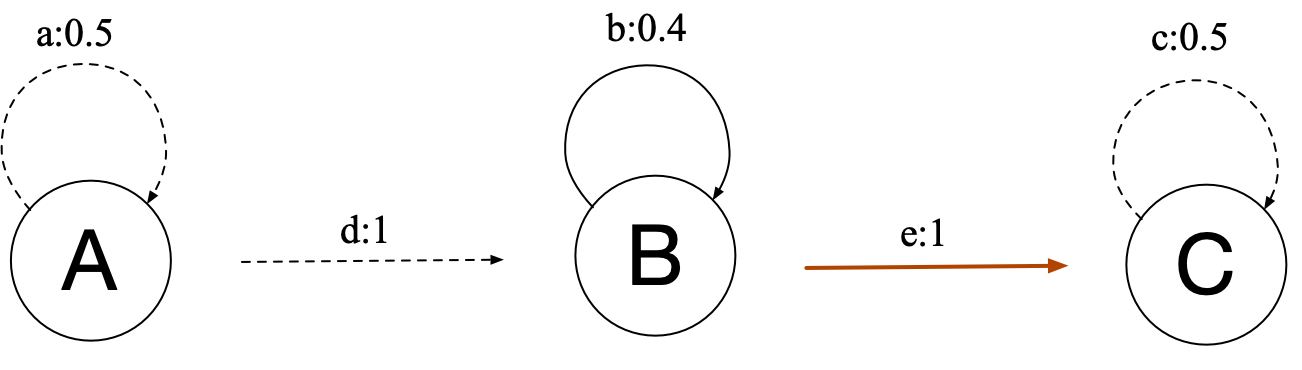
\includegraphics[width=\linewidth]{sasim/nonsubmodular_sample1.png}
        \caption{边$b$,$e$被选中\label{fig:nonsub_a}}
    \end{subfigure}
    \quad
    \begin{subfigure}[t]{0.44\linewidth}
        \centering
        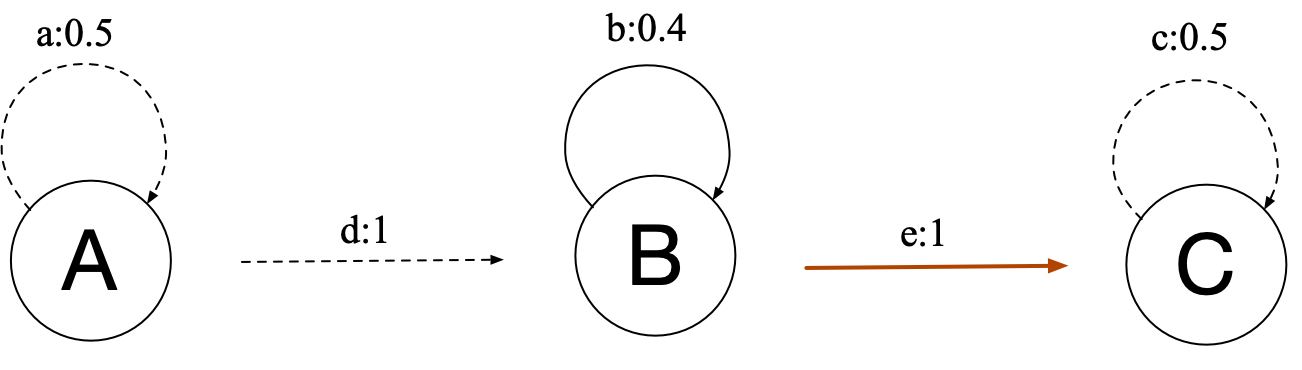
\includegraphics[width=\linewidth]{sasim/nonsubmodular_sample1.png}
        \caption{边$a$,$b$,$d$,$e$被选中\label{fig:nonsub_b}}
    \end{subfigure}

    \caption{\label{fig:nonsub_sample}函数$h$不满足子模性举例}
\end{figure}


然而,目标函数$h$并{\bfseries 不满足子模性},这一点很容易通过举反例得到。

如图\ref{fig:nonsub_sample}所示,节点$A$、$B$、$C$是可以选择推荐的三个广告,每条边上的数字,如果该边是自环,则代表用户愿意接受该广告的概率,如果是非自环,则代表用户接受边的头部节点对尾部节点的增益倍率。我们先把问题简化为只有一个轮次$t$, 并且用户网络中只有一个用户节点$u$,所有广告单次点击收益均为$1$。在此例中,由于$u$和$t$的值是相同的,为了方便,我们暂时用$p_{v}$代表$p_{u,v,t}$,用图中边上的小写字母代表边两侧的节点和时间的三元组,如$a$表示$(A,A,t)$。

图\ref{fig:nonsub_a}中虚线边代表该边未被选中,黑实线边代表已被选中,计算棕色实线边$e$的边际收益$h(e|\{b\})$。先算每个被推荐的广告被接受的概率:$p_B=0.4$,$h(\{b\})=p_B \cdot revenue(B)=0.4$。加入边$e$后,广告$C$也会被推荐,$p_C=0.4 \cdot 1 \cdot 0.5=0.2$,虽然如果推荐了$C$,最终边$c$一定也会在边集里,但此时我们只计算$e$带来的收益,所以要忽略掉用户本身对广告$C$的接受程度,不计算边$c$的收益。$h(\{b,e\})=p_B\cdot revenue(B)+p_C\cdot revenue(C)=0.4\cdot 1+0.2\cdot 1=0.6$。在图\ref{fig:nonsub_a}的情况下,$e$的边际收益为$h(e|\{b\})=h(\{b,e\})-h(\{e\})=0.2$。

图\ref{fig:nonsub_b}中的图结构与图\ref{fig:nonsub_a}中一致,但是多选择了两条边$a,b$,同样地,计算棕色实线边$e$的边际收益$h(e|{a,b,d})$。$p_A=0.5$,$p_B=0.4+0.5\cdot 1\cdot 0.4=0.6$,$h(\{a,b,d\})=p_A\cdot revenue(A)+p_B\cdot revenue(B)=0.5\cdot 1 + 0.6 \cdot 1 = 1.1$。$p_C=0.6 \cdot 1\cdot 0.5 = 0.3$,$h(\{a,b,d,e\})=1.4$。$h(e|{a,b,d})=h(\{a,b,d,e\})-h(\{a,b,d\})=1.4-1.1=0.3$。

$h(e|\{b\})\le h(e|\{a,b,d\})$,显然不满足子模性。直观地理解,子模性一般代表边际收益随答案集合变大而递减,在这个例子中,$e$的价值会随着$B$被接受的概率提高而提高,答案集合的变大又导致了$B$被接受的概率提高,那么$e$的收益就随着答案集合变大而提升了,显然不满足子模性,所以对于我们上述问题中的函数$h$,并不能满足定理\ref{thm:greedy}。

对于满足单调性但不满足子模性的目标函数,为了保证算法具有合理的近似比,需要引入\parencite{sandwich}中提到的三明治算法来解决,先令:

\begin{equation}
\Delta_t^\rho(\sigma_t)=\Delta h_t(E(\sigma_t))=h(E(\bigcup_{i=1}^{t-1}{\sigma_i} \cup \sigma_t)) - h(E(\bigcup_{i=1}^{t-1}{\sigma_i}))
\end{equation}

\begin{equation}
\Delta_t^\mu(\sigma_t)=\Delta h_t^\mu(E(\sigma_t))=h_t^\mu(E(\bigcup_{i=1}^{t-1}{\sigma_i} \cup \sigma_t)) - h_t^\mu(E(\bigcup_{i=1}^{t-1}{\sigma_i}))
\end{equation}

\begin{equation}
\Delta_t^\nu(\sigma_t)=\Delta h_t^\nu(E(\sigma_t))=h_t^\nu(E(\bigcup_{i=1}^{t-1}{\sigma_i} \cup \sigma_t)) - h_t^\nu(E(\bigcup_{i=1}^{t-1}{\sigma_i}))
\end{equation}

在每一个轮次$t$,都需要找到两个与$h$定义在同样定义域上的子模函数$h_t^\mu$和$h_t^\nu$,满足对于定义域上的任意$E_t' \subseteq \{(v_1,v_2,t_0)|(v_1,v_2,t_0)\in E',t_0=t\}$,都有$\Delta h_t^\mu(E') \le \Delta h_t(E') \le \Delta h_t^\nu(E')$。即$\Delta h_t^\mu$处处是$\Delta h_t$的下界,$\Delta h_t^\nu$处处是$\Delta h_t$的上界,并且如果将原问题中的$h$替换为$h_t^\mu$和$h_t^\nu$,且每一轮得到的结果近似比均至少每一轮得到的结果近似比至少不差于原问题。

将三明治算法应用于边贪心算法,如算法\ref{alg:sandwich}所示。每一轮分别使用$h_t^\mu$、$h$和$h_t^\nu$($h_t^\mu$和$h_t^\nu$会在后文中定义)替换原来的$h$来运行三次贪心算法,得到三个结果,$\sigma_t^\mu$,$\sigma_t^\rho$和$\sigma_t^\nu$,然后在其中选择一个最好的作为最终结果:$\sigma_t^{sand}=\arg\max_{\sigma_t \in \{\sigma_t^\mu,\sigma_t^\rho,\sigma_t^\nu\}}\Delta_\rho(\sigma_t)$。在每一轮中使用三明治算法,并将结果加入到答案中,最终得到$\sigma$。

\begin{algorithm}
    \caption{三明治算法\label{alg:sandwich}} 
    \begin{algorithmic}[1]
        \REQUIRE 用户网络, $G(U,E)$; 广告网络, $N(V,W)$; 时间轮, $T$; 预算 $k$; 函数 $h,h_t^\mu,h_t^\nu:2^{|E|} \times T \to \mathbb{R} $
        \ENSURE $\sigma$
        \STATE Let $\sigma \gets \phi$
        \FOR{$t=1$ to $T$}
            \STATE 使用$h_t^\mu$,$h$,$h_t^\nu$分别代替$h$执行算法\ref{alg:edge_greedy}中的\ref{alg:greedy_line4}-\ref{alg:greedy_line5}行,得到$\sigma_t^\mu$,$\sigma_t^\rho$,$\sigma_t^\nu$
            \STATE $\sigma_t^{sand}=\arg\max_{\sigma_t \in \{\sigma_t^\mu,\sigma_t^\rho,\sigma_t^\nu\}}\Delta_\rho(\sigma_t)$
            \STATE $\sigma = \sigma \cup \{\sigma_t^{sand}\}$
        \ENDFOR
    \end{algorithmic}
\end{algorithm}

根据\parencite{sandwich}中三明治算法近似比的证明,我们可以得到:

\begin{theorem}
\label{thm:sand}
三明治方法保证对任意$t \in [T]$,使用多轮反向影响力采样的边贪心算法有:

\begin{equation}
    \Delta_\rho(\sigma_t^{sand}) \ge \max\left\{\frac{\Delta_\rho(\sigma_t^\nu)}{\Delta_\nu(\sigma_t^\nu)},\frac{\Delta_\mu(\sigma_t^{\rho*})}{\Delta_\rho(\sigma_t^{\rho*})} \right\} \cdot (\frac{1-e^{-(1-\frac{1}{k})}}{2d_{in}+1})\cdot \Delta_\rho(\sigma_t^{*})
\end{equation}
\end{theorem}

\noindent 其中$\sigma_t^{*}$代表$\Delta_\rho$在第$t$轮的最优解。

定义函数$h_t^\mu$和$h_t^\nu$,除计算第$t$轮的$p_{u,v,t}$以外,其余部分与函数$h$均一致,只需重新定义用户在第$t$轮对所推荐广告的接受概率计算部分,即:
\begin{align}
    &p_{u,v,t}^\mu=\mathbb{I}\{(v,v,t)\in E(\sigma_t)\}\cdot w(u,(v,v)) \label{equ:def_mu}\\
    &p_{u,v,t}^\nu=\mathbb{I}\{(v,v,t)\in E(\sigma_t)\}\cdot w(u,(v,v)) + \max_{(v',v,t)\in E(\sigma_t)}\{w(u,(v',v))\}\cdot w(u,(v,v)) \label{equ:def_nu}
\end{align}

直观地理解,函数$h_t^\mu$和$h_t^\nu$限制了当前轮由于边的增加导致的某些边对其他的点的增益增大的情况下,在其余条件都相同的情况下,函数$h_t^\mu$在计算某个广告被接受的概率时,不考虑边的增益,只计算每个节点本身的价值,相当于去除了边的增强作用,最终得到的结果一定小于原函数值。函数$h_t^\nu$则是默认前面的广告被接受的概率均为$1$,增大了这些广告对该广告增益的概率,最终得到的结果一定大于原函数值,因此有$\Delta h_t^\mu(E_t') \le \Delta h_t(E_t') \le \Delta h_t^\nu(E_t')$。

\begin{lemma}
\label{lem:mon_sub}
函数$\Delta h_t^\mu$和$ \Delta h_t^\nu$在其定义域上都是单调并子模的。
\end{lemma}

\noindent 证明:与引理\ref{lem:h_mon}类似,单调性较为显然。我们找到的$\Delta h_t^\mu$和$ \Delta h_t^\nu$,边不会由于新边的加入而体现出更大的价值,反之会稀释其增益,导致边际收益随着集合的增大而下降,直观上是满足子模性的。具体理论证明如下:

令$\mathcal{W}_t=\{(v_1,v_2,t_0) |(v_1,v_2,t_0) \in \mathcal{W},t_0=t\}$。

要证明$\Delta h_t^\mu$单调性,即证明:对于任意的集合$A \subseteq \mathcal{W}_t$和边$(v_1,v_2,t_0) \in \mathcal{W}_t\setminus A$,都有$\Delta h_t^\mu(A)\le \Delta h_t^\mu(A\cup\{(v_1,v_2,t_0)\})$;

要证明$\Delta h_t^\mu$子模性,即证明:对于任意两个集合$A\subseteq B \subseteq \mathcal{W}_t$和边$(v_1,v_2,t_0) \in \mathcal{W}_t \setminus B$,都有$\Delta h_t^\mu(A \cup \{(v_1,v_2,t_0)\})-\Delta h_t^\mu(A) \ge \Delta h_t^\mu(B\cup \{(v_1,v_2,t_0)\})- \Delta h_t^\mu(B)$;对于$h_t^\nu$也一样,把上标换成$\nu$即可。

为了方便,我们使用$p_{u,v,t}^{\mu,A}$和$p_{u,v,t}^{\mu,A'}$分别代表在$h_t^\mu(A)$和$h_t^\mu(A\cup\{(v_1,v_2,t_0)\})$边集下,用户$u$在第$t$轮接受广告$v$的概率,即式\ref{equ:def_mu}中所定义的$p_{u,v,t}^\mu$的含义。对于$\nu$和$B$也是类似的。

根据定义,加入一条边$(v_1,v_2,t_0)$,只会改变第$t$轮中用户们对$v_2$的 接受概率。也就是, 当$t\ne t_0$或者$v \ne v_2$时$p_{u,v,t}^{\mu,A}=p_{u,v,t}^{\mu,A'}$,$p_{u,v,t}^{\nu,A}=p_{u,v,t}^{\nu,A'}$。

若$v_1=v_2$:
\begin{equation}
p_{u,v_2,t_0}^{\mu,A'}-p_{u,v_2,t_0}^{\mu,A}=p_{u,v_2,t_0}^{\mu,B'}-p_{u,v_2,t_0}^{\mu,B} =w(u,(v_2,v_2)) \ge 0
\end{equation}
\begin{equation}
p_{u,v_2,t_0}^{\nu,A'}-p_{u,v_2,t_0}^{\nu,A}=p_{u,v_2,t_0}^{\nu,B'}-p_{u,v_2,t_0}^{\nu,B} =w(u,(v_2,v_2)) \ge 0
\end{equation}
若$v_1 \ne v_2$:

\begin{equation}
    p_{u,v_2,t_0}^{\mu,A'}-p_{u,v_2,t_0}^{\mu,A}=p_{u,v_2,t_0}^{\mu,B'}-p_{u,v_2,t_0}^{\mu,B} = 0 
\end{equation}
\begin{align}
    p_{u,v_2,t_0}^{\nu,A'}-p_{u,v_2,t_0}^{\nu,A}&=\mathbb{I}\{w(u,(v_1,v_2))>\max_{(v',v_2,t)\in A}\{w(u,(v',v_2))\}\} \cdot [w(u,(v_1,v_2)) \nonumber \\ 
    & \ \ \ \ \ -\max_{(v',v_2,t)\in A}\{w(u,(v',v_2))\}] \cdot w(u,(v_2,v_2)) \ge  0
\end{align}

因为$A \subseteq B$,所以$\max_{(v',v_2,t)\in A}\{w(u,(v',v_2))\} \le \max_{(v',v_2,t)\in B}\{w(u,(v',v_2))\}$。

若$w(u,(v_1,v_2))\le \max_{(v',v_2,t)\in A}\{w(u,(v',v_2))\}$:$p_{u,v_2,t_0}^{\nu,A'}-p_{u,v_2,t_0}^{\nu,A}=p_{u,v_2,t_0}^{\nu,B'}-p_{u,v_2,t_0}^{\nu,B}=0$;

若$\max_{(v',v_2,t)\in A}\{w(u,(v',v_2))\} < w(u,(v_1,v_2)) \le \max_{(v',v_2,t)\in B}\{w(u,(v',v_2))\}$:
\begin{equation}
p_{u,v_2,t_0}^{\nu,A'}-p_{u,v_2,t_0}^{\nu,A}\ge 0 = p_{u,v_2,t_0}^{\nu,B'}-p_{u,v_2,t_0}^{\nu,B}
\end{equation}

若$w(u,(v_1,v_2)) > \max_{(v',v_2,t)\in B}\{w(u,(v',v_2))\}$:
\begin{align}
    (p_{u,v_2,t_0}^{\nu,A'}&-p_{u,v_2,t_0}^{\nu,A})-(p_{u,v_2,t_0}^{\nu,B'}-p_{u,v_2,t_0}^{\nu,B}) \\ 
    &=[\max_{(v',v_2,t)\in B}\{w(u,(v',v_2))\} - \max_{(v',v_2,t)\in A}\{w(u,(v',v_2))\}] \cdot w(u,(v_2,v_2)) \\
    &\ge 0
\end{align}

综上,对于任意的集合$A \subseteq \mathcal{W}_t$和边$(v_1,v_2,t_0) \in \mathcal{W}_t\setminus A$,有

\begin{equation}
    p_{u,v_2,t_0}^{\mu,A} \le p_{u,v_2,t_0}^{\mu,A'},p_{u,v_2,t_0}^{\nu,A} \le p_{u,v_2,t_0}^{\nu,A'}
\end{equation}

同引理\ref{lem:h_mon}可得,$\Delta h_t^\mu$和$\Delta h_t^\nu$是单调的。

接下来证明子模性。对于任意两个集合$A\subseteq B \subseteq \mathcal{W}_t$和边$(v_1,v_2,t_0) \in \mathcal{W}_t \setminus B$,有
\begin{equation}
    p_{u,v_2,t_0}^{\mu,A'}-p_{u,v_2,t_0}^{\mu,A}\ge  p_{u,v_2,t_0}^{\mu,B'}-p_{u,v_2,t_0}^{\mu,B}
\end{equation}
\begin{equation}
    p_{u,v_2,t_0}^{\nu,A'}-p_{u,v_2,t_0}^{\nu,A}\ge  p_{u,v_2,t_0}^{\nu,B'}-p_{u,v_2,t_0}^{\nu,B}
\end{equation}

把$p_{u,v_2,t_0}^{\mu,A'}$、$p_{u,v_2,t_0}^{\mu,A}$和$p_{u,v_2,t_0}^{\mu,B'}$、$p_{u,v_2,t_0}^{\mu,B}$分别代入引理\ref{lem:h_mon}证明中的式\ref{equ:mon2}中得:
\begin{align}
    &(\Delta h_{t,i}^{\mu}(A)-\Delta h_{t,i-1}^{\mu}(A)) - (\Delta h_{t,i}^{\mu}(B)-\Delta h_{t,i-1}^{\mu}(B)) \\ 
    &=revenue(v_2)\cdot (\sum_{\mathcal{S}_{v_2}\subseteq \mathcal{U}\setminus \{(i,t_0)\}}\left[Pr_{i-1}^{\mu,A}(\mathcal{S}_{v_2})\cdot\frac{p_{i,v_2,t_0}^{\mu,A'}-p_{i,v_2,t_0}^{\mu,A}}{1-p_{i,v_2,t_0}^{\mu,A}} \cdot g(\{(i,t_0)\} |\mathcal{S}_{v_2})\right] \nonumber \\
    & \  \ \ \ \ \ \ - \sum_{\mathcal{S}_{v_2}\subseteq \mathcal{U}\setminus \{(i,t_0)\}}\left[Pr_{i-1}^{\mu,B}(\mathcal{S}_{v_2})\cdot\frac{p_{i,v_2,t_0}^{\mu,B'}-p_{i,v_2,t_0}^{\mu,B}}{1-p_{i,v_2,t_0}^{\mu,B}} \cdot g(\{(i,t_0)\} |\mathcal{S}_{v_2})\right] )\\ 
    &\ge revenue(v_2)\cdot (p_{i,v_2,t_0}^{\mu,A'}-p_{i,v_2,t_0}^{\mu,A})  
    \cdot \sum_{\mathcal{S}_{v_2}\subseteq \mathcal{U}\setminus \{(i,t_0)\}}\left[\left(\frac{Pr_{i-1}^{\mu,A}(\mathcal{S}_{v_2})}{1-p_{i,v_2,t_0}^{\mu,A}}-\frac{Pr_{i-1}^{\mu,B}(\mathcal{S}_{v_2})}{1-p_{i,v_2,t_0}^{\mu,B}}\right) \cdot g(\{(i,t_0)\} |\mathcal{S}_{v_2})\right] \label{equ:prof_sub1}
\end{align}

为了方便,我们对$\mathcal{S}_v$中的每一个$(u,t)$进行标号,标号由$1$到$|\mathcal{U}|。$用$(u_j,t_j)$代表的标号为$j$的$(u,t)$对,即$idx(u_j,t_j)=j$。

令:$p_{u,v,t}^{\mu,A,i}=\begin{cases}p_{u,v,t}^{\mu,A'}, u<i,\\p_{u,v,t}^{\mu,A},u\ge i \end{cases}$

那么,对于任意的$u,v,t,i$,都有$p_{u,v,t}^{\mu,A,i} \le p_{u,v,t}^{\mu,B,i}$。

设:
\begin{equation}
\footnotesize
    Pr_{i,j}^{\mu,A,B}(\mathcal{S}_v)=\left(\prod_{{(u,t)\in \mathcal{S}_v \atop idx(u,t)\le j } \atop{ idx(u,t) \ne idx(i,t_0)}}p_{u,v,t}^{\mu,B,i}\right)\cdot \left(\prod_{{(u,t) \notin \mathcal{S}_v \atop idx(u,t)\le j} \atop{ idx(u,t) \ne idx(i,t_0)}} (1-p_{u,v,t}^{\mu,B,i})\right)
    \cdot \left(\prod_{{(u,t)\in \mathcal{S}_v \atop idx(u,t)> j} \atop {idx(u,t)\ne idx(i,t_0)}}p_{u,v,t}^{\mu,A,i}\right)\cdot \left(\prod_{{(u,t) \notin \mathcal{S}_v \atop idx(u,t)> j} \atop{ idx(u,t)\ne idx(i,t_0)}} (1-p_{u,v,t}^{\mu,A,i})\right)
\end{equation}

根据定义,则有式\ref{equ:prof_sub1}中的$Pr_{i,0}^{\mu,A,B}(\mathcal{S}_{v2})=\frac{Pr_{i-1}^{\mu,A}(\mathcal{S}_{v_2})}{1-p_{i,v_2,t_0}^{\mu,A}}$,$Pr_{i,|\mathcal{U}|}^{\mu,A,B}(\mathcal{S}_{v2})=\frac{Pr_{i-1}^{\mu,B}(\mathcal{S}_{v_2})}{1-p_{i,v_2,t_0}^{\mu,B}}$。

设:
\begin{align}
    H_{i,j}^{\mu}(A,B)&= \sum_{\mathcal{S}_{v_2}\subseteq \mathcal{U} \setminus \{(i,t_0)\}}\left[Pr_{i,j}^{\mu,A,B}(\mathcal{S}_{v_2}) \cdot g(\{(i,t_0)\} |\mathcal{S}_{v_2})\right],i\ne j 
    \\H_{i,j}^{\mu}(A,B)&=H_{i,j-1}^{\mu}(A,B),i=j
\end{align}

当$i=j$且$j>0$时,$H_{i,j}^{\mu}(A,B)-H_{i,j-1}^{\mu}(A,B)=0$。

当$i \ne j$且$j>0$时:
\begin{align}
\small
    &H_{i,j}^{\mu}(A,B)-H_{i,j-1}^{\mu}(A,B) \nonumber \\
    &=\sum_{\mathcal{S}_{v_2}\subseteq \mathcal{U} \setminus \{(i,t_0),(u_j,t_j)\}}[(Pr_{i,j}^{\mu,A,B}(\mathcal{S}_{v_2}) \cdot g(\{(i,t_0)\} |\mathcal{S}_{v_2})\nonumber \\
    &\ \ \ \ + Pr_{i,j}^{\mu,A,B}(\mathcal{S}_{v_2}\cup\{(u_j,t_j)\}) \cdot g(\{(i,t_0)\} |\mathcal{S}_{v_2}\cup \{(u_j,t_j)\})) \nonumber \\ 
    &\ \ \ \ -\left(Pr_{i,j-1}^{\mu,A,B}(\mathcal{S}_{v_2}) \cdot g(\{(i,t_0)\} |\mathcal{S}_{v_2})+Pr_{i,j-1}^{\mu,A,B}(\mathcal{S}_{v_2}\cup\{(u_j,t_j)\}) \cdot g(\{(i,t_0)\} |\mathcal{S}_{v_2} \cup \{(u_j,t_j)\})\right)] \\ 
    &=\sum_{\mathcal{S}_{v_2}\subseteq \mathcal{U} \setminus \{(i,t_0),(u_j,t_j)\}}[Pr_{i,j-1}^{\mu,A,B}(\mathcal{S}_{v_2})\cdot \left(\frac{1-p_{u_j,v_2,t_j}^{\mu,B,i}}{1-p_{u_j,v_2,t_j}^{\mu,A,i}} - 1\right) \cdot g(\{(i,t_0)\} |\mathcal{S}_{v_2})\nonumber\\
    &\ \ \ \ +Pr_{i,j-1}^{\mu,A,B}(\mathcal{S}_{v_2}\cup\{(u_j,t_j)\})\cdot \left(\frac{p_{u_j,v_2,t_j}^{\mu,B,i}}{p_{u_j,v_2,t_j}^{\mu,A,i}}-1\right) \cdot g(\{(i,t_0)\} |\mathcal{S}_{v_2} \cup \{(u_j,t_j)\})] \\  
    &=\sum_{\mathcal{S}_{v_2}\subseteq \mathcal{U} \setminus \{(i,t_0),(u_j,t_j)\}}[Pr_{i,j-1}^{\mu,A,B}(\mathcal{S}_{v_2})\cdot \left(\frac{1-p_{u_j,v_2,t_j}^{\mu,B,i}}{1-p_{u_j,v_2,t_j}^{\mu,A,i}} - 1\right) \cdot g(\{(i,t_0)\} |\mathcal{S}_{v_2})\nonumber\\
    &\ \ \ \ +Pr_{i,j-1}^{\mu,A,B}(\mathcal{S}_{v_2})\cdot \frac{p_{u_j,v_2,t_j}^{\mu,A,i}}{1-p_{u_j,v_2,t_j}^{\mu,A,i}} \cdot \left(\frac{p_{u_j,v_2,t_j}^{\mu,B,i}}{p_{u_j,v_2,t_j}^{\mu,A,i}}-1\right) \cdot g(\{(i,t_0)\} |\mathcal{S}_{v_2}\cup \{(u_j,t_j)\})] \\
    &= \sum_{\mathcal{S}_{v_2}\subseteq \mathcal{U} \setminus \{(i,t_0),(u_j,t_j)\}}\left[Pr_{i,j-1}^{\mu,A,B}(\mathcal{S}_{v_2})\cdot \frac{p_{u_j,v_2,t_j}^{\mu,B,i}-p_{u_j,v_2,t_j}^{\mu,A,i}}{1-p_{u_j,v_2,t_j}^{\mu,A,i}} \cdot (g(\{(i,t_0)\} |\mathcal{S}_{v_2} \cup \{(u_j,t_j)\})-g(\{(i,t_0)\} |\mathcal{S}_{v_2}))\right] \\
    &\le 0 \label{equ:prof_sub2}
\end{align}

式\ref{equ:prof_sub2}的不等号由$p_{u,v,t}^{\mu,A,i} \le p_{u,v,t}^{\mu,B,i}$和$g(\{(i,t_0)\} |\mathcal{S}_{v_2} \cup \{(u_j,t_j)\})-g(\{(i,t_0)\} |\mathcal{S}_{v_2}) \le 0$得。函数$g$已被证明是子模的\cite{mrim},因此有$g(\{(i,t_0)\} |\mathcal{S}_{v_2} \cup \{(u_j,t_j)\})\le g(\{(i,t_0)\} |\mathcal{S}_{v_2}) $。

所以对于任意的$0<i\le |U_S|$和$0<j\le |\mathcal{U}|$均有:$H_{i,j}^{\mu}(A,B)-H_{i,j-1}^{\mu}(A,B) \le 0$,因此$H_{i,0}^{\mu} (A,B)\ge H_{i,1}^{\mu}(A,B) \ge H_{i,1}^{\mu}(A,B) \ge \ldots \ge H_{i,|\mathcal{U}|}^{\mu}(A,B)$。

根据定义,
\begin{equation}
H_{i,0}^{\mu} (A,B)= \sum_{\mathcal{S}_{v_2}\subseteq \mathcal{U}\setminus \{(i,t_0)\}}\left[\frac{Pr_{i-1}^{\mu,A}(\mathcal{S}_{v_2})}{1-p_{i,v_2,t_0}^{\mu,A}} \cdot g(\{(i,t_0)\} |\mathcal{S}_{v_2})\right]
\end{equation}

\begin{equation}
H_{i,|\mathcal{U}|}^{\mu} (A,B)= \sum_{\mathcal{S}_{v_2}\subseteq \mathcal{U}\setminus \{(i,t_0)\}}\left[\frac{Pr_{i-1}^{\mu,B}(\mathcal{S}_{v_2})}{1-p_{i,v_2,t_0}^{\mu,B}} \cdot g(\{(i,t_0)\} |\mathcal{S}_{v_2})\right]
\end{equation}

又因为$p_{i,v_2,t_0}^{\mu,A'}\ge p_{i,v_2,t_0}^{\mu,A}$,所以
\begin{equation}
(\ref{equ:prof_sub1})=revenue(v_2)\cdot (p_{i,v_2,t_0}^{\mu,A'}-p_{i,v_2,t_0}^{\mu,A})\cdot H_{i,0}^{\mu}(A,B)-(H_{i,|\mathcal{U}|}^{\mu}(A,B)) \ge 0
\end{equation}

即对于所有的$0<i \le |U_S|$,$(\Delta h_{t,i}^{\mu}(A)-\Delta h_{t,i-1}^{\mu}(A)) - (\Delta h_{t,i}^{\mu}(B)-\Delta h_{t,i-1}^{\mu}(B)) \ge 0$,所以
\begin{align}
    [\Delta h_t^\mu(A \cup \{(v_1,v_2,t_0)\}&-\Delta h_t^\mu(A))]- [\Delta h_t^\mu(B\cup \{(v_1,v_2,t_0)\})-\Delta h_t^\mu(B)]\\ 
    &=\sum_{i=1}^{|U_S|}[(\Delta h_{t,i}^{\mu}(A)-\Delta h_{t,i-1}^{\mu}(A)) - (\Delta h_{t,i}^{\mu}(B)-\Delta h_{t,i-1}^{\mu}(B))] \ge 0
\end{align}

$\Delta h_t^\mu$子模性得证。同理可得$\Delta h_t^\nu$也是子模的。

\noindent 证明完毕。

\section{近似性与复杂度分析}
\label{sec:ana}

针对\ref{sec:def}节中定义的多轮社交广告序列影响最大化问题,\ref{sec:greedy}节给出了基于广告边的贪心策略。\ref{sec:mrris}节中提出的多轮反向影响力采样算法能够解决估算广告边在社交网络中造成的影响力的问题,保证算法的时间复杂度。\ref{sec:sand}节使用三明治算法解决了原问题函数$h$不子模的问题,保证了算法的近似性。将多轮反向影响力采样算法和三明治算法应用于边贪心策略,才能在保证复杂度和近似性的情况下解决多轮社交广告序列影响最大化问题。

\begin{theorem}
\label{thm:nonadptive}
对任意的$\varepsilon>0$和$\ell > 0$,使用多轮反向影响力采样和三明治方法的边贪心算法得到的$\sigma$至少有$1-\frac{1}{n^{\ell}}$的概率满足:
\begin{equation}
\frac{\rho(\sigma)}{\rho(\sigma*)} \ge 1-e^{-\min_{t \in [T]}\left\{\max\left\{\frac{\Delta_\rho(\sigma_t^\nu)}{\Delta_\nu(\sigma_t^\nu)},\frac{\Delta_\mu(\sigma_t^{\rho*})}{\Delta_\rho(\sigma_t^{\rho*})} \right\}\right\}\cdot\left(\frac{1-e^{-(1-\frac{1}{k})}}{2d_{in}+1}-\varepsilon\right)}
\end{equation}
\end{theorem}

\noindent 证明:结合定理\ref{thm:greedy}和引理\ref{lem:ris},可得,使用多轮反向影响力采样的边贪心算法每轮至少有$1-\frac{1}{n^{\ell}}$能得到近似比为$\frac{1-e^{-(1-\frac{1}{k})}}{2d_{in}+1}$的结果。按照三明治算法的过程,每一轮用$h^\mu$和$h^\nu$代替$h$执行原算法过程,然后取最优结果作为每一轮的最终结果,结合定理\ref{thm:sand}和引理\ref{lem:mon_sub},则每轮至少有$1-\frac{1}{n^{\ell}}$的概率,可以得到近似比为$\max\left\{\frac{\Delta_\rho(\sigma_t^\nu)}{\Delta_\nu(\sigma_t^\nu)},\frac{\Delta_\mu(\sigma_t^{\rho*})}{\Delta_\rho(\sigma_t^{\rho*})} \right\}\cdot\left(\frac{1-e^{-(1-\frac{1}{k})}}{2d_{in}+1}-\varepsilon\right)$的近似结果。易知,将每个$\sigma_t$作为元素的集合函数$\rho$仍然是单调子模的,因此,套用定理\ref{thm:greedy}证明中提到的$1-e^{-\alpha}$的结论,即可得到定理\ref{thm:nonadptive}。

\noindent 证明完毕。

纵观算法过程,使用了多轮反向影响力采样方法和三明治方法的边贪心的时间复杂度为$O\left(\frac{(Tk^2 m_v n + m_u)Tn_u(\ell \ln n_u + \ln (2T))}{\varepsilon^2}\cdot\frac{R}{LB_{\min}}\right)$,其中$m_v=|W|$代表广告网络的边数,$m_u=|E|$代表用户网络边数,$n_u=|G|$为用户网络节点数,$n_s=|U_S|$为特殊用户集合大小,$R$与$LB$含义与引理\ref{lem:ris}中一致,$LB_{\min}$代表$LB$可能得最小值。算法需进行$T$轮,每轮至多$k$次选边,选边需遍历大小为$m_v$的广告边集,在估算一条边的边际收益时,需要遍历$\theta$个多轮反向可达集,统计采样结果需要计算已经被选择的广告,不会超过$Tk$个,只要统计有哪些特殊用户在该广告出现的那一轮接受了这个广告即可,因此统计其结果的时间为$Tkn_S$,总复杂度为$O(T^2k^2m_vn_S\theta)$。对于生成采样的部分,沿用上一次生成过的采样结果不会影响其估算的准确性,故只需按照最大的$\theta$生成一次即可。生成一个采样的时间是$Tm_u$,这部分时间复杂度为$O(\theta Tm_u)$。综上,根据引理\ref{lem:ris},代入$\theta$,总时间复杂度即为$O(Tkm_v\cdot Tk(n_u+m_u)\theta) = O\left(\frac{(Tk^2 m_v n + m_u)Tn_u(\ell \ln n_u + \ln (2T))}{\varepsilon^2}\cdot\frac{R}{LB_{\min}}\right)$。


\section{动态多轮社交广告序列影响最大化}
\label{sec:ada}

在部分实际场景中,在算法进行每一轮决策后,可以观测用户对广告的接受情况和在用户网络中的传播结果。在这种允许动态观测的情况下,可以收集这些信息做出更准确的判断。令$ A_t = \{(u,v) |  u \in U, v \in V ,u \text{在前}t\text{轮接受过广告}v\} $ 代表前t轮广告序列信息在用户网络中传播的观测结果。则动态多轮社交广告序列影响最大化问题的目标则是找到 $\sigma_t = arg max_{\sigma_t} \Delta(E(\sigma_t) | A_{t-1})$,即$\Delta(E(\sigma_t) | A_{t-1})$为每一轮需要最大化的目标函数:
\begin{equation}
    \Delta(E(\sigma_t) | A_{t-1}) = \sum_{v \in V} ( f(E(\sigma_t), v) \cup \{u | (u,v) \ in A_{t-1}\}) \cdot revnue(v) - \sum_{(u,v) \in A_{t-1}} revenue(v) 
\end{equation}

针对动态多轮社交广告序列影响最大化,我们提出了动态边贪心策略,如算法\ref{alg:ada}所示。算法结构整体上与非动态的贪心算法\ref{alg:edge_greedy}类似,只需在估算边际收益时考虑到$A_{t-1}$的信息,并且在每一轮传播后更新新一轮用户对广告的接受情况$A_{t}$。

同样的,在动态观测情况下,也需要使用多轮反向影响力采样加速估计广告边的边际收益。当使用算法\ref{alg:mrris}估算$v$的边际收益时,如果一个多轮反向可达集的其实节点为$u$,且$(u,v) \in A_{t-1}$,则跳过第\ref{alg:mrrisline1}到\ref{alg:mrrisline2}行,使这个多轮反向可达集的贡献为$1$。如果$(u,v) \notin A_{t-1}$,当$t_0 < t$时,令$p_{u,v,t_0} = 0$。这样可以保证估算结果准确性的同时复用多轮反向影响力算法生成的多轮反向可达集。

\begin{algorithm}[H]
    \caption{动态边贪心算法\label{alg:ada}}
    \begin{algorithmic}[1]
        \REQUIRE 用户网络 $G(U,E)$; 广告网络 $N(V,W)$; 预算 $k$; $t-1$轮的观测结果$A_{t - 1}$
        \STATE \(\sigma_t \gets ( )\)
        \WHILE{\( |\sigma_t| \le k-2 \)}
            \STATE \(\mathcal{E} = \{(v_i,v_j) \in W | v_j \notin \sigma_t \}\)
            \IF{\(\mathcal{E} = \phi\)}
                \STATE 跳出循环
            \ENDIF
            \STATE \(\forall (v_i,v_j) \in \mathcal{E}\) 计算 $\Delta({(v_i,v_j,t)} \cup E(\sigma_t)|A_{t-1})$
            \STATE \((v_i,v_j) = \mathop{\arg\max}_{(v_i,v_j) \in \mathcal{E}}\Delta({(v_i,v_j,t)} \cup E(\sigma_t)|A_{t-1}) \)
            \IF{\(v_j=v_i\) 或 \(v_i \in \sigma_t\)}
                \STATE \(\sigma_t = \sigma_t \oplus v_j\)
            \ELSE
                \STATE \(\sigma_t = \sigma_t \oplus v_i \oplus v_j\) 
            \ENDIF
        \ENDWHILE
        \STATE 观察 $\sigma_t$的传播结果,更新 $A_t$。
    \end{algorithmic}
\end{algorithm}

\ref{sec:sand}节中对$h$的分析,同样使用于动态情况下的目标函数$\Delta$,因此也需要使用三明治方法,分别使用$\Delta_\mu$、$\Delta$、$\Delta_\nu$运行算法\ref{alg:ada}得到三个结果然后取最优。同样地,$\Delta_\mu$和$\Delta_\nu$的定义与$\Delta$类似,只需依照$h_\mu$和$h_\nu$的定义,修改$p_{u,v,t}$的计算方法即可。

\begin{theorem}
令$\sigma_t^*$为动态多轮社交广告序列影响最大化的最优解,则对于任意的$\varepsilon>0$和$\ell > 0$,使用多轮反向影响力采样和三明治方法的动态边贪心算法得到的$\sigma_t$至少有$1-\frac{1}{n^{\ell}}$的概率满足:

\begin{equation}
    \frac{\Delta(E(\sigma_t) | A_{t-1})}{\Delta(E(\sigma_t^*) | A_{t-1})}
    \ge \max\left\{\frac{\Delta_\rho(E(\sigma_t^\nu) | A_{t-1} )}{\Delta_\nu(E(\sigma_t^\nu) | A_{t-1})},\frac{\Delta_\mu(E(\sigma_t^{\rho*})  | A_{t-1})}{\Delta_\rho(E(\sigma_t^{\rho*}) | A_{t-1})} \right\}
    \cdot\left(\frac{1-e^{-(1-\frac{1}{k})}}{2d_{in}+1}-\varepsilon\right)
\end{equation}

\noindent 算法的时间复杂度为$O\left(\frac{(Tk^2 m_v n + m_u)Tn_u(\ell \ln n_u + \ln (2T))}{\varepsilon^2}\cdot\frac{R}{LB_{\min}}\right)$。证明方法与定理\ref{thm:nonadptive}相同,不再赘述。
\end{theorem}

\section{本章小结}

在本章中,首先在\ref{sec:def}节中,同时考虑广告网络中广告之间的关联关系和用户网络中的信息传播,提出并定义了的多轮社交广告序列影响最大化问题。在\ref{sec:greedy}节中提出了基于广告边的贪心算法。由于目标函数无法快速精确计算,为估计每一条的边际收益,\ref{sec:mrris}节设计了适合多轮广告序列影响最大化问题的多轮反向影响力采样方法。然后在\ref{sec:sand}节引入三明治方法,找到了合适的上界函数和下界函数,解决变函数不具备子模性的问题。在\ref{sec:ana}节中分析了将多轮反向影响力采样算法和三明治算法应用于边贪心算法解决多轮社交广告序列影响力最大化问题的近似性和时间复杂度。\ref{sec:ada}节在原问题的基础上考虑到可以动态观测广告在用户网络中传播结果的情况,拓展了多轮社交广告序列影响力最大化问题并给出对应的贪心算法。

\chapter{实验设计与结果分析}

% 由于鲁棒序列网络子模最大化问题和多轮社交广告序列影响最大化问题的目标函数计算方法差异较大,需要对数据集进行的预处理也不相同,本章将分为分别介绍对应的实验细节和结果。

\section{鲁棒序列网络子模最大化算法实验}
\label{sec:5_1}

\subsection{实验数据集}

{\bfseries Amazon评论数据集}:我们基于亚马逊视频游戏评论数据集\cite{ni2019justifying}进行了广告推荐实验。实验的具体目标是,给定用户已经购买的商品,预测他们接下来可能想购买的商品为它们推荐广告。

为此,我们构建了一个图模型$N = (V,W)$。其中,$V$代表所有产品的集合,$W$表示产品之间的边集。每条边的权重$w_{ij}$定义为条件概率:即用户在购买产品$i$后购买产品$j$的概率。我们通过计算所有购买过产品$i$的用户中,随后又购买产品$j$的用户比例来确定$w_{ij}$。此外,图中还包含自环,其权重$w_{ii}$表示在所有用户中购买产品$i$的比例。为了确保数据的可靠性,我们只考虑了被购买至少50次的商品,最终得到9383种独立商品。同时,我们选取了至少购买过29种商品的用户,共909名。我们对这909名用户进行广告推荐任务,并计算每个评估指标的平均值来衡量推荐效果。

{\bfseries Wikispeedia数据集}:我们使用Wikispeedia数据集\cite{west2009wikispeedia},考虑用户在维基百科中浏览并通过链接跳转试图找到某个目标文章的情况。我们的任务是,根据用户之前访问过的一系列文章,预测并为他们推荐链接,引导他们到达目标页面。这个任务的关键在于页面访问顺序,因为不同页面拥有不同的有效链接。具体而言,我们会基于用户访问的前4个页面,预测他们接下来点击的链接和试图到达的页面。

我们构建了一个图模型$N = (V,W)$。其中$V$代表所有页面的集合,$W$表示页面之间现有链接的集合。对于每条边$(i,j)\in W$,其权重$w_{ij}$定义为条件概率:即用户当前在页面$i$的情况下移动到页面$j$的概率。这个概率通过计算从$i$到$j$的移动次数占所有访问$i$次数的比例来得出。值得注意的是,我们没有构建自环,因为我们假设用户只能通过现有链接进行页面间的跳转,而不能随机访问页面。我们将数据集压缩为仅包含出现在实际浏览路径中的文章和边,最终得到4170个独立页面和55147条边。我们选取了长度至少为29的路径进行分析,共得到271条符合条件的路径。我们对这271条路径进行链接预测任务,并计算每个评估指标的平均值来衡量预测效果。



\subsection{实验设置与评估标准}

为了有效评估和对比算法的性能,我们使用了三个评估指标:

\begin{itemize}
    \item \textbf{准确度得分}:这个指标简单地计算准确推荐项目的数量,是一个很合理的衡量标准,但它的局限性在于没有明确考虑序列的顺序。
    \item \textbf{序列得分}:为了弥补准确度得分的不足,我们引入了基于Kendall-Tau距离\cite{kendall1938new}的度量。它通过计算在预测序列和真实序列中都出现的有序对的数量来评估序列的相似度。这个指标更好地反映了推荐序列的质量。
    \item \textbf{目标函数值}:我们采用如下概率价值函数作为目标网络子模函数$f$:
\begin{equation}
    f(\sigma)=h(E(\sigma))=\sum_{j\in V} [1- \prod_{(i,j)\in E(\sigma)} (1-w_{ij})]
\end{equation}
\end{itemize}

前两个指标在\parencite{mitrovic2019adaptive}中也有使用。对于全部的评估指标,我们会尝试对$\sigma$所有大小为$\tau$的子集进行移除,选择最低的得分或函数值作为最终评估指标,以衡量序列的稳定性。

我们对以下算法的性能进行对比:

\begin{itemize}
\item {\bfseries 鲁棒序列}:本文提出的鲁棒序列网络子模最大化算法,简称鲁棒序列算法。
\item {\bfseries 序列贪心}:序列贪心算法\cite{mitrovic2018submodularity},不考虑序列的鲁棒性。
\item {\bfseries OMegA}:现有的子模序列基准算法\cite{tschiatschek2017selecting}。
\item {\bfseries 高频推荐}:较为平凡的基准算法,推荐最受欢迎的(用户点击最多的)项目(商品广告或链接)。
\end{itemize}

为了探究加入鲁棒参数$\tau$后得到的结果在不移除情况下的表现,实验中还会额外对比两项结果:
\begin{itemize}
\item {\bfseries 鲁棒序列($\tau = 0$)}:本文提出的鲁棒序列网络子模最大化算法,在算法运行时,正常使用$\tau$作为鲁棒参数,但在评估时不会对结果中的节点进行选择性移除。即只有评估时$\tau = 0$。
\item {\bfseries 序列贪心($\tau = 0$)}:序列贪心算法,在评估时不会对结果中的节点进行选择性移除,即评估时$\tau = 0$。
\end{itemize}



对于在Amazon评论数据集上进行的广告推荐实验,设置$k\in[11,20],\tau \in[0,10]$。算法会根据用户已购买的前$4$个产品,预测其接下来可能购买的$k$个产品。

对于Wikispeedia数据集上进行的链路预测实验,设置$k\in[6,15],\tau \in[0,10]$。算法会根据用户前面点击的$4$个链接,预测其接下来可能想要点击的$k$个链接。


\subsection{对比实验结果}

图\ref{fig:rec}展示了几种算法在广告推荐任务中的表现,分别从准确度得分、序列得分和目标函数值三个方面进行了比较。在图\ref{fig:rec-acc}、\ref{fig:rec-acc-t}、\ref{fig:rec-seq}和\ref{fig:rec-seq-t}中,我们观察到在移除$\tau$个元素后,鲁棒序列算法的性能优于所有对比算法。考虑到准确度分数和序列分数是实际应用中常用的评估指标,这一结果充分证明了鲁棒序列算法在广告推荐任务中的有效性和鲁棒性。

图\ref{fig:rec-fun}和\ref{fig:rec-fun-t}有区别的是,当$\tau$较小或$k$较大时,OMegA算法表现更为出色。OMegA算法致力于寻找全局最优解,它在每次选择元素后都会对所有候选对象进行拓扑重排。当$k$较大且$\tau$较小时,OMegA能够返回具有更优目标函数值的解,但其运行速度显著慢于鲁棒序列和序列贪心算法,而且OMegA在准确度和序列分数方面的表现相对较差。综合考虑,鲁棒序列算法在实际应用中仍然展现出更高的效率和鲁棒性。

我们还特别关注了鲁棒序列和序列贪心算法在$\tau=0$时的情况。可能需要解释的一点是,在图\ref{fig:rec-acc-t}、\ref{fig:rec-seq-t}和\ref{fig:rec-fun-t}中,序列贪心($\tau=0$)由于算法运行与$\tau$无关,且评估时固定$\tau=0$,所以结果成一条直线。而鲁棒序列($\tau=0$)由于在算法运行时仍然会正常使用$\tau$,因此即使评估时固定$\tau=0$,得出的结果也会随$\tau$变化而变化。

实验结果显示,在目标函数值方面,序列贪心($\tau=0$)略胜一筹;但在准确度分数和序列分数上,鲁棒序列($\tau=0$)与序列贪心($\tau=0$)的表现非常接近,有时甚至更优。序列贪心($\tau=0$)在目标函数值上的优势源于贪心框架的有效性。鲁棒序列算法虽然独立调用了两次序列贪心算法,但由于网络子模性的影响,难以达到单次序列贪心执行的性能水平。然而,准确度和序列分数上的结果表明,直接应用贪心选择并非总是最优策略。这反映了贪心算法的内在特性:尽管$1-1/e$接近最佳近似比,但在特定场景下,某些启发式算法可能会取得更好的表现。
\begin{figure}[H]
    \centering
    \begin{subfigure}{0.45\textwidth}
        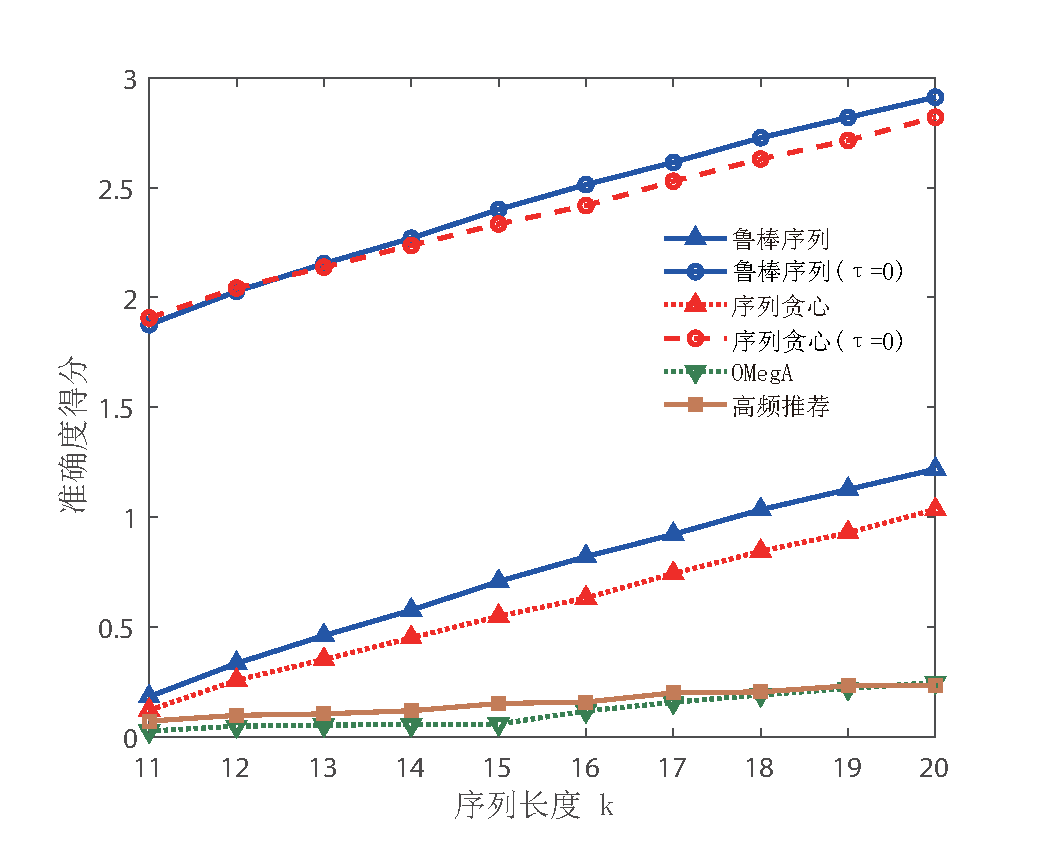
\includegraphics[width=\linewidth]{figure/rosenets/rec/rec-acc1}
        \caption{$\tau=10$ and $k=[11,20]$}
        \label{fig:rec-acc}
    \end{subfigure}
    \hfill
    \begin{subfigure}{0.45\textwidth}
        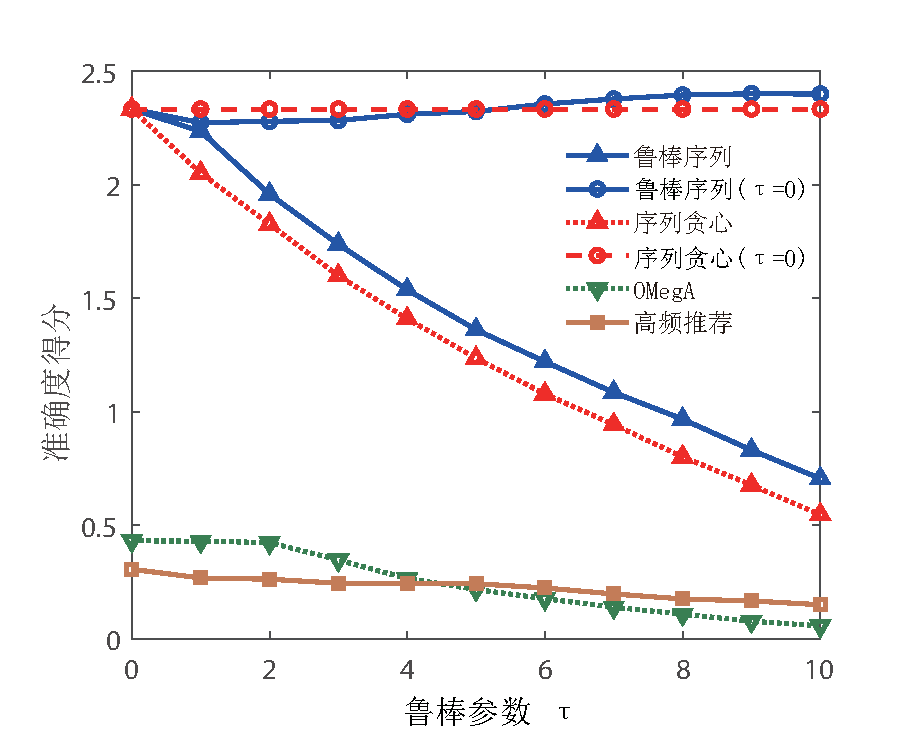
\includegraphics[width=\linewidth]{figure/rosenets/rec/rec-acc1-t}
        \caption{$k=15$ and $\tau=[0,10]$}
        \label{fig:rec-acc-t}
    \end{subfigure}

    \medskip

    \begin{subfigure}{0.45\textwidth}
       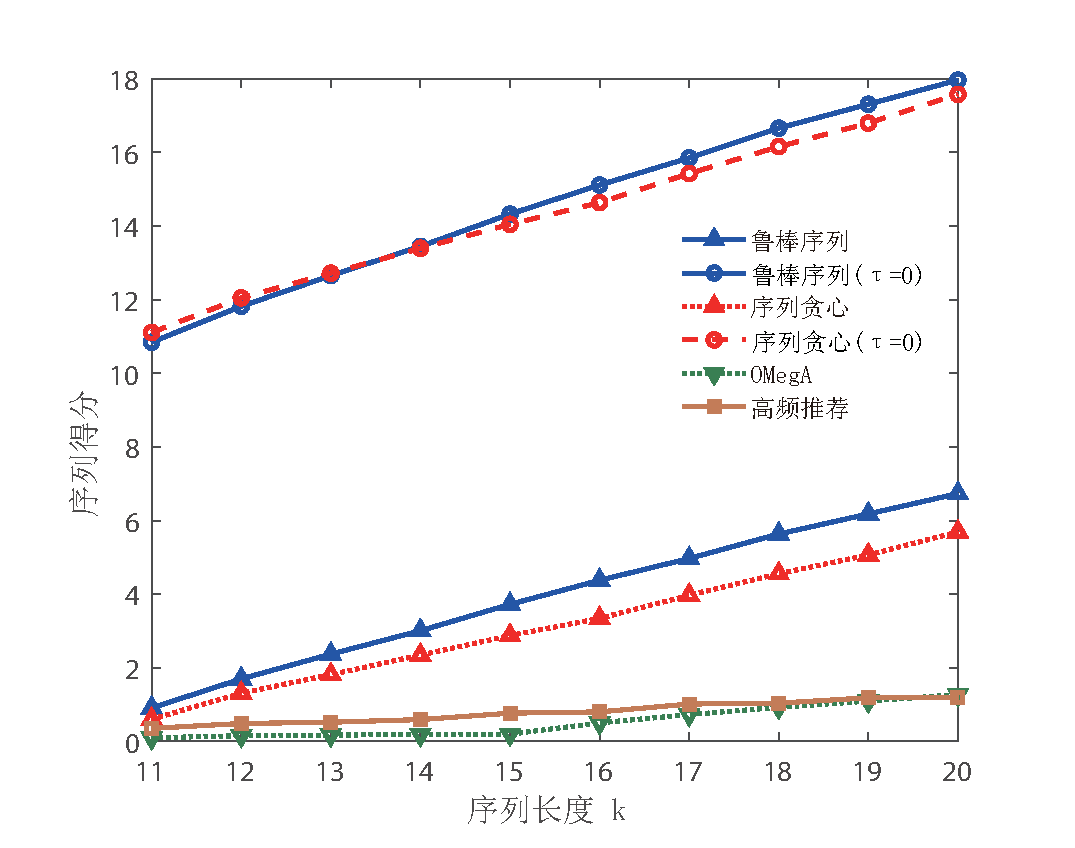
\includegraphics[width=\linewidth]{figure/rosenets/rec/rec-seq1}
        \caption{$\tau=10$ and $k=[11,20]$}
        \label{fig:rec-seq}
    \end{subfigure}
    \hfill
    \begin{subfigure}{0.45\textwidth}
        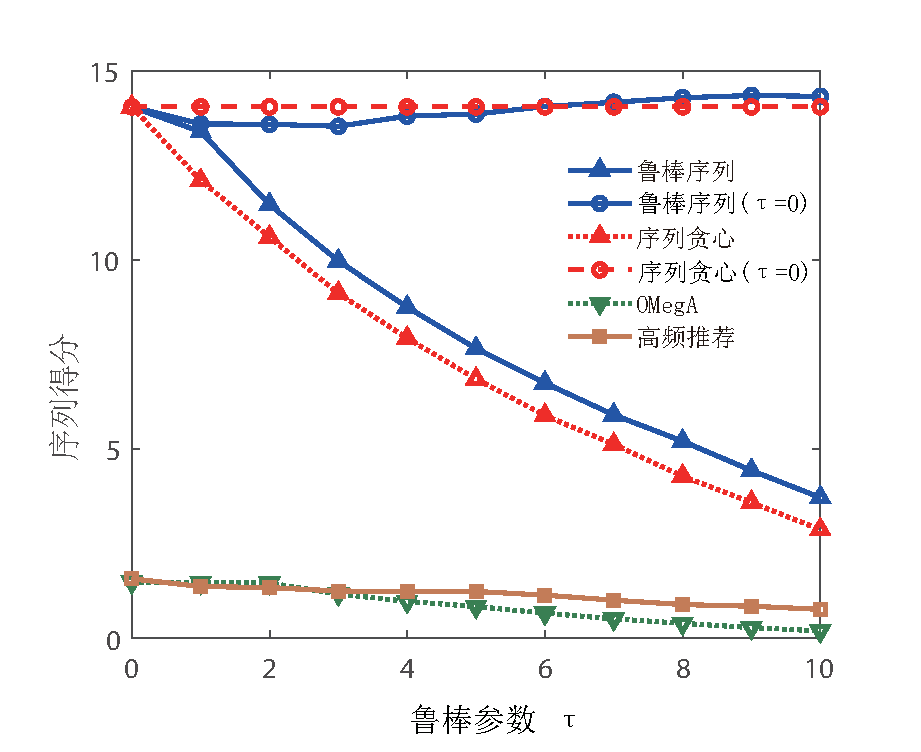
\includegraphics[width=\linewidth]{figure/rosenets/rec/rec-seq1-t}
        \caption{$k=15$ and $\tau=[0,10]$}
        \label{fig:rec-seq-t}
    \end{subfigure}

    \medskip

    \begin{subfigure}{0.45\textwidth}
       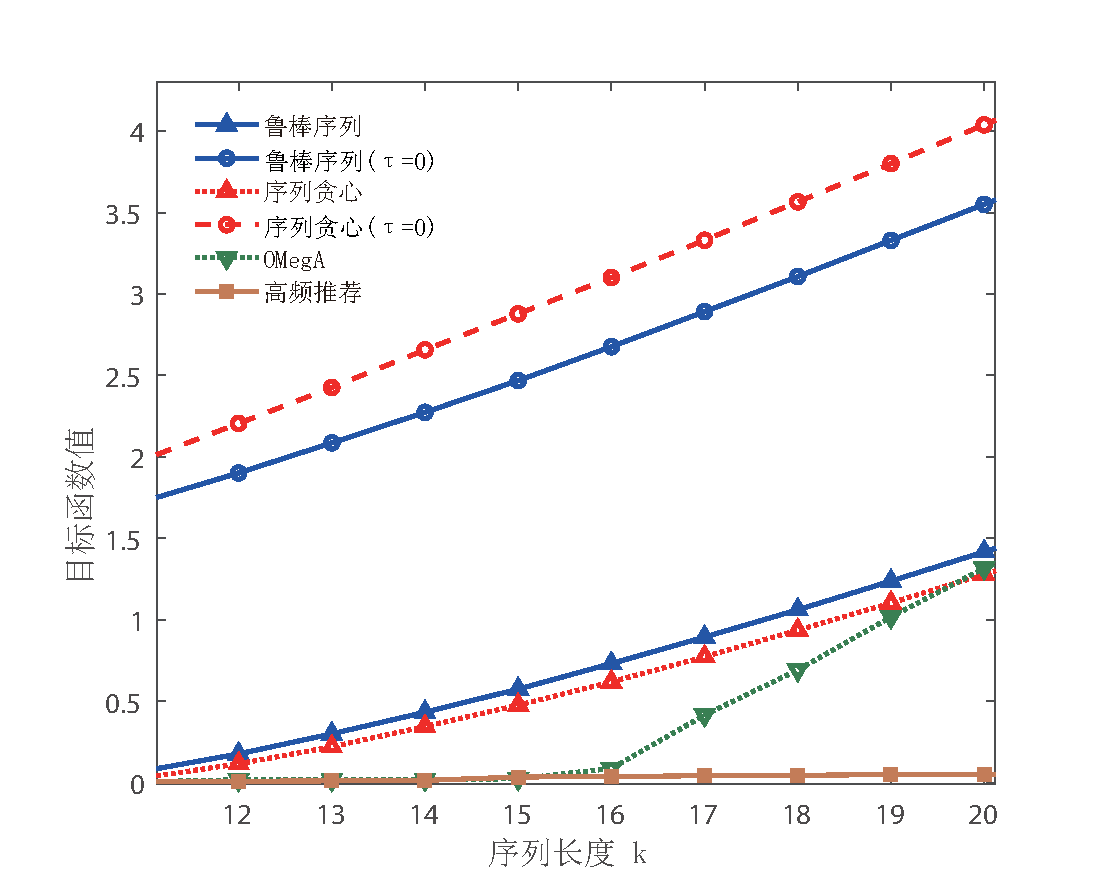
\includegraphics[width=\linewidth]{figure/rosenets/rec/rec-fun1}
        \caption{$\tau=10$ and $k=[11,20]$}
        \label{fig:rec-fun}
    \end{subfigure}
    \hfill
    \begin{subfigure}{0.45\textwidth}
        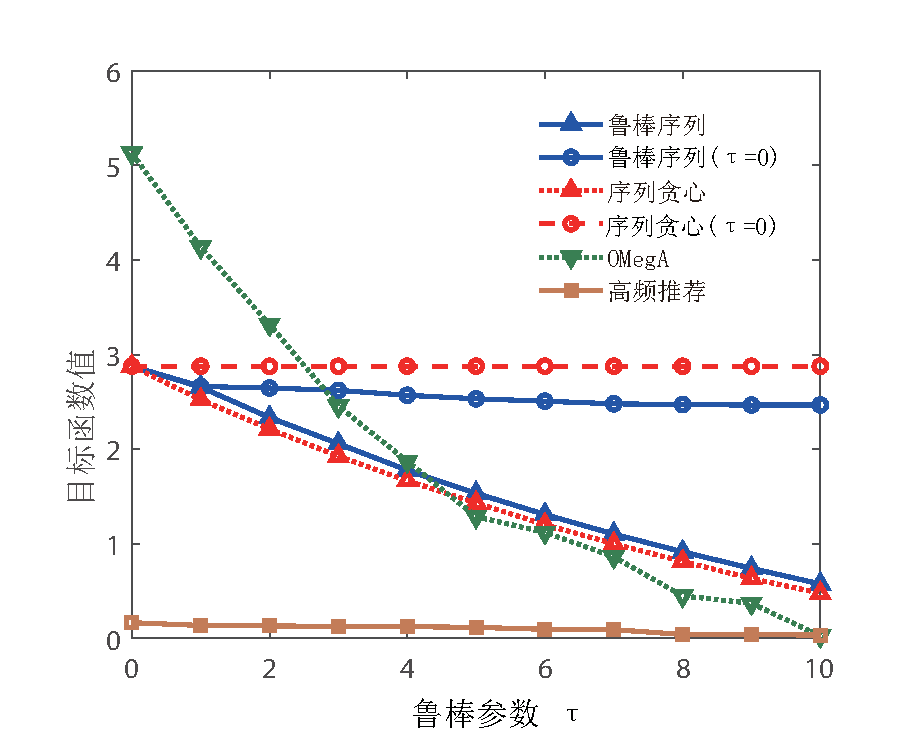
\includegraphics[width=\linewidth]{figure/rosenets/rec/rec-fun1-t}
        \caption{$k=15$ and $\tau=[0,10]$}
        \label{fig:rec-fun-t}
    \end{subfigure}
    \caption{广告推荐实验结果\label{fig:rec}}
\end{figure}

值得一提的是,如果我们增加序列贪心算法的调用次数,可能会获得更鲁棒的实验结果和更高的近似比,但目标函数值可能会下降。这是因为多次独立的贪心选择会增加触发收益递减现象的概率。在实际应用中,设计鲁棒算法时面临的一个关键挑战是如何在算法的鲁棒性和目标函数值最大化之间取得平衡。这需要我们根据具体应用场景和需求,权衡各种因素,以达到最佳的综合效果。

\begin{figure}[H]
    \centering
    \begin{subfigure}{0.45\textwidth}
        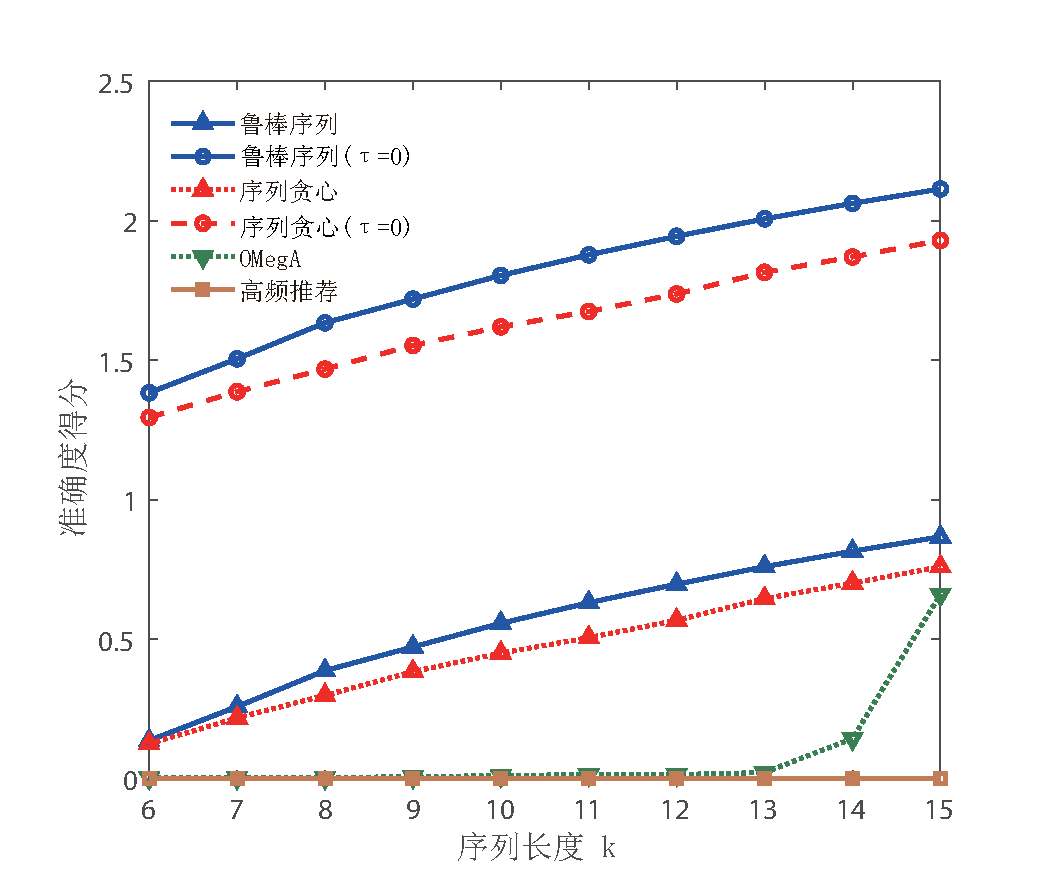
\includegraphics[width=\linewidth]{figure/rosenets/wik/wik-acc}
        \caption{$\tau=5$ and $k=[6,15]$}
        \label{fig:wik-acc}
    \end{subfigure}
    \hfill
    \begin{subfigure}{0.45\textwidth}
        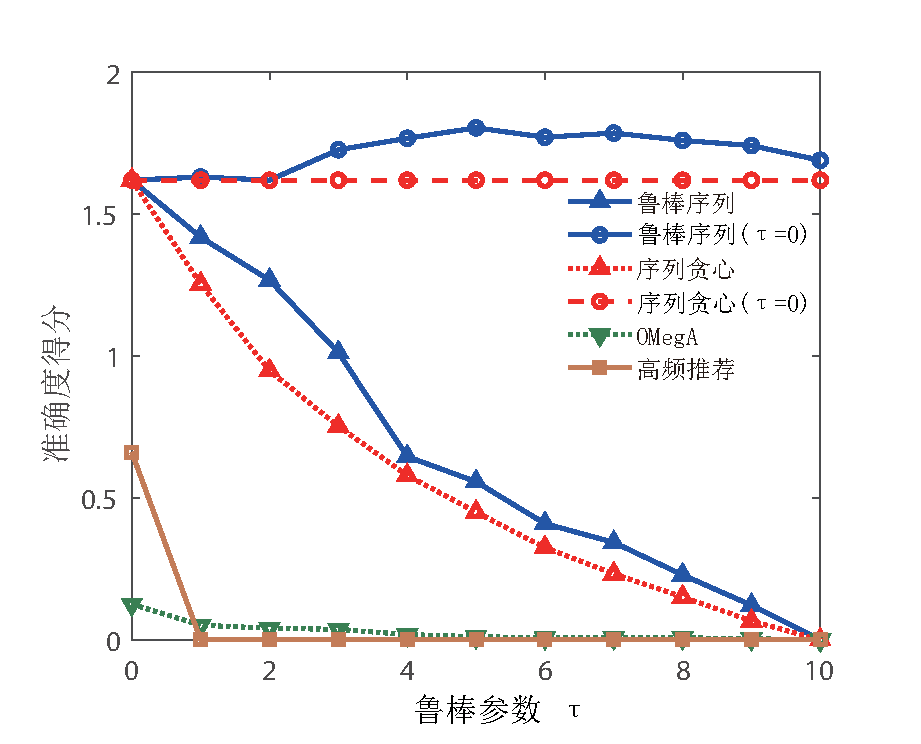
\includegraphics[width=\linewidth]{figure/rosenets/wik/wik-acc-t}
        \caption{$k=10$ and $\tau=[0,10]$}
        \label{fig:wik-acc-t}
    \end{subfigure}

    \medskip

    \begin{subfigure}{0.45\textwidth}
       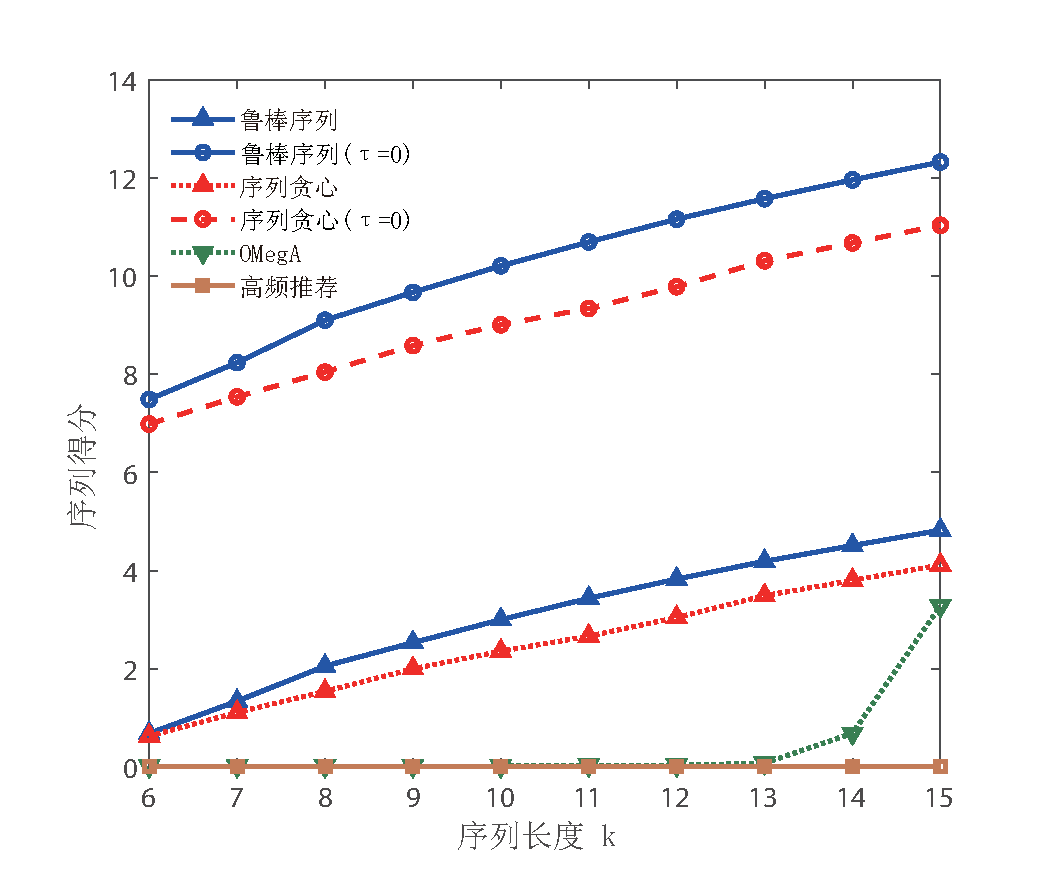
\includegraphics[width=\linewidth]{figure/rosenets/wik/wik-seq}
        \caption{$\tau=5$ and $k=[6,15]$}
        \label{fig:wik-seq}
    \end{subfigure}
    \hfill
    \begin{subfigure}{0.45\textwidth}
        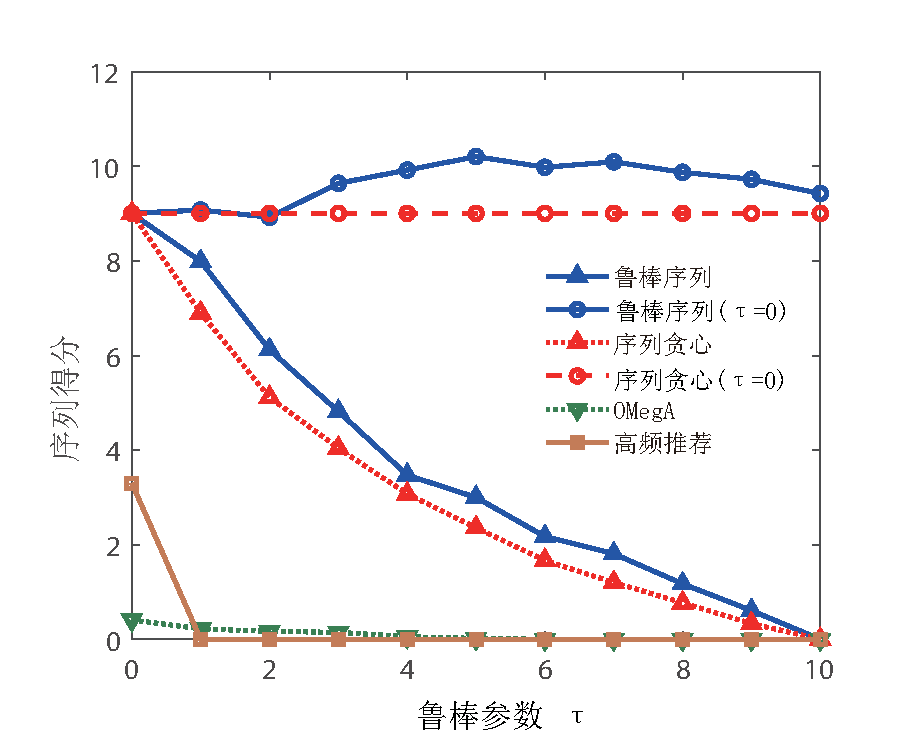
\includegraphics[width=\linewidth]{figure/rosenets/wik/wik-seq-t}
        \caption{$k=10$ and $\tau=[0,10]$}
        \label{fig:wik-seq-t}
    \end{subfigure}

    \medskip

    \begin{subfigure}{0.45\textwidth}
       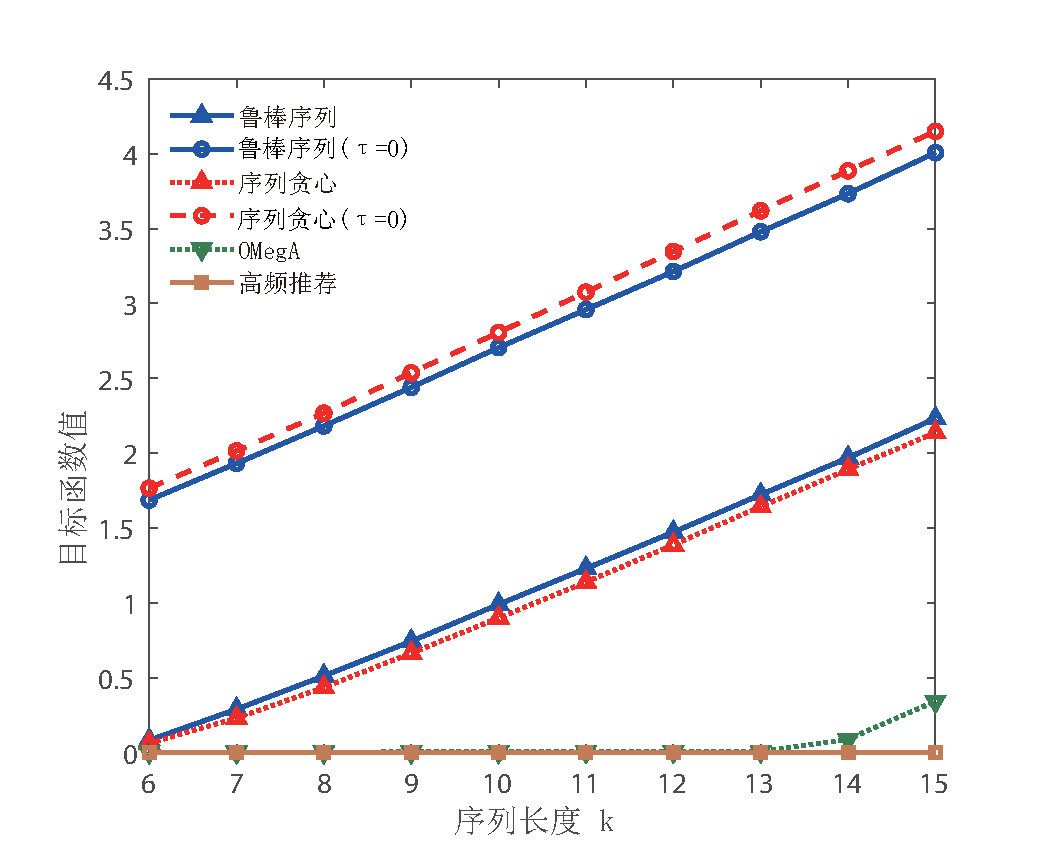
\includegraphics[width=\linewidth]{figure/rosenets/wik/wik-fun}
        \caption{$\tau=5$ and $k=[6,15]$}
        \label{fig:wik-fun}
    \end{subfigure}
    \hfill
    \begin{subfigure}{0.45\textwidth}
        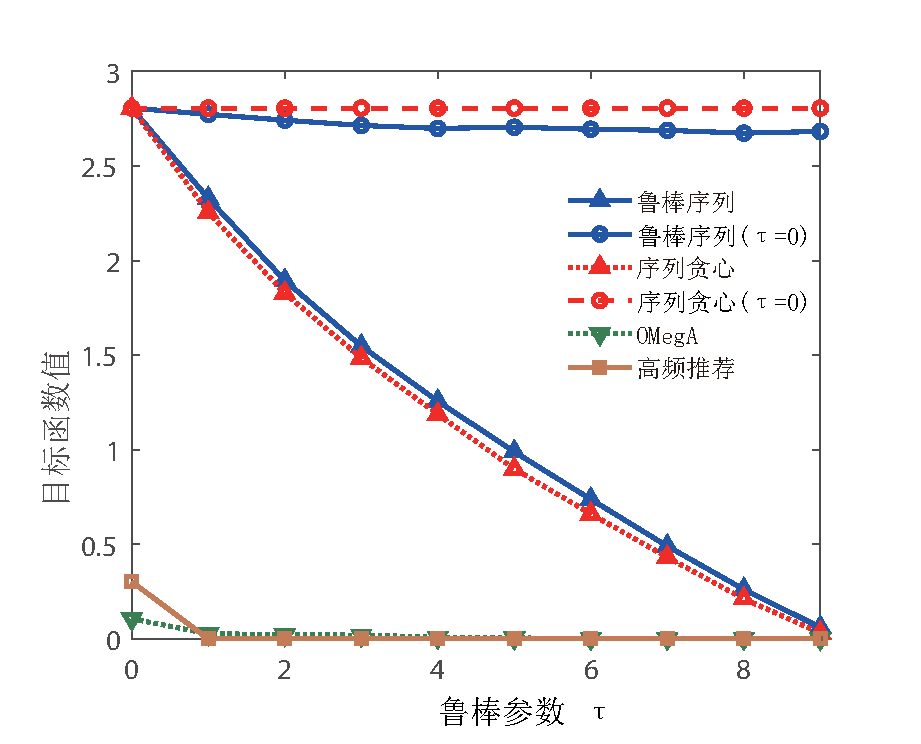
\includegraphics[width=\linewidth]{figure/rosenets/wik/wik-fun-t}
        \caption{$k=10$ and $\tau=[0,10]$}
        \label{fig:wik-fun-t}
    \end{subfigure}
    \caption{链路预测实验结果\label{fig:wik}}
\end{figure}

图\ref{fig:wik}分别几种算法在链路预测中的表现,分别从准确度得分、序列得分和目标函数值三个方面进行了比较。我们发现在移除$\tau$个元素后,鲁棒序列在所有情况下都优于所有比较对象。这些结果表明鲁棒算法在链路预测任务中是有效且鲁棒的。与广告推荐实验不同的是,OMegA算法在这项任务中未能展现出与鲁棒序列算法相当的性能。这主要归因于两个因素:首先,本任务中需要预测的路径通常较长;其次,不同路径之间的交叉部分相对较少,不如广告推荐实验中那样普遍。这些特点使得全局算法OMegA难以充分发挥其优势。而且我们可以在图\ref{fig:wik-acc},\ref{fig:wik-seq}和4\ref{fig:wik-fun}中发现,当$k$变大时,OMegA算法的性能增长更快。这反过来证明了鲁棒序列算法更加通用、有效和鲁棒,能够适应不同的应用场景,而无需对特定环境做出假设。

链接预测应用中的另一个不同之处是,鲁棒序列($\tau=0$)在准确度和序列分数方面几乎在所有情况下都优于序列贪心($\tau=0$)。这再次验证了直接实施贪心选择有时可能远离最优解。因此,我们认为探索如何通过增加独立贪心选择试验的次数,在算法的鲁棒性、效率和目标函数值最大化之间取得更好的平衡也是一个有趣的未来探索方向。



\section{多轮社交广告序列影响最大化推荐算法实验}
\label{sec:5_2}

\subsection{实验数据集}

多轮广告序列推荐实验在{\bfseries Amazon评论数据集}\cite{amazon24}上进行。该数据集主要记录了用户对已经购买的商品的评论信息。商品网络和用户网络的生成参考了Gomez-Rodriguez等人\cite{netgen}的工作。如果较多买过商品$i$的人还买过商品$j$,说明$i$和$j$有较大关联性,就在商品网络中加入一条由$i$到$j$的有向边,并对每一个商品都加入自环;如果两个用户多次购买过相同的商品,那么可以推断他们更有可能是朋友,就在他们之间增加一条有向边。

在触发模型中,还需要对用户网络的每一条边进行赋权,简单地使每条边在$[0,1]$中生成一个随机权重$b_{u_1,u_2}$。为了传播的效果更好并体现用户区分度,对于每个用户网络,都选择度数较大的5个节点和度数较小的5个节点作为特殊用户组$U_S$。对于每一个商品$v$,我们在$\{0.01,0.02,0.03,0.04,0.05\}$中随机一个值作为$revenue(v)$。每个用户对于商品的接受程度不同,首先对每个特殊用户$u$和商品的每个自环$(v,v)$,都在$[0,1]$范围内随机生成一个$w(u,(v,v))$代表用户$u$对商品$v$的接受程度。然后对于每个特殊用户$u$和商品的每条非自环边$(v_1,v_2)$,都在$[0,1/w,(u,(v_2,v_2))-1]$范围内随机生成一个$w(u,(v_1,v_2))$代表用户$u$接受了$v_1$对$v_2$的接受概率的促进程度。

Amazon评论数据集对于不同的商品类别分开统计。我们按照用户网络和广告网络的稠密程度以及节点与边的规模挑选不同类别,生成了4个不同大小的数据集,数据集的具体参数见表\label{tab:imdata}。

\begin{table}[htbp]
	\setlength{\tabcolsep}{2mm}{}
	\centering
	\normalsize
	\caption{数据集参数}\label{tab:imdata}
	\begin{tabular}[t]{|c|c|c|c|c|}
        \hline
		Dataset Name & 用户个数 & 用户边数 & 广告个数 & 广告边数 \\ \hline
		Gift\_Cards & 1477 & 50000 & 306 & 13122 \\ \hline
		Software & 1573 & 20000 & 2032 & 107429 \\ \hline
		Magazine\_Subscriptions & 854 & 36566 & 1125 & 17381 \\ \hline
		Video\_Games & 3230 & 300000 & 1613 & 202573 \\ \hline
	\end{tabular}	
\end{table}

\subsection{参数设定}

实验设置$T=5$,$k=10$,即每次实验进行$5$轮,每一轮选择至多$10$个广告。对算法选出的序列进行$10000$次蒙特卡洛模拟,将收益结果的平均值作为评价标准,对于动态观测的情况,则以观测到的最终收益结果作为评价标准。

算法中多轮反向影响力采样部分有两个参数$\varepsilon$和$\ell$,可以通过调整这两个参数来控制算法的准确度和运行效率。$\varepsilon$越小,$\ell$越大,算法在估计每条边的边际收益时就越准确,同时运行时间也会越长。观察算法的流程,可以发现调整参数$\varepsilon$和$\ell$的最终效果都只是改变了$\theta$的大小,因此分别设置$\theta=10,100,1000,10000,100000$运行边贪心算法,记录分析其多轮反向采样得到的目标函数估计值、对结果进行$10000$次蒙特卡洛模拟得到的期望收益以及运行时间。

\begin{figure}[th]
    \centering
    \begin{subfigure}{0.45\textwidth}
        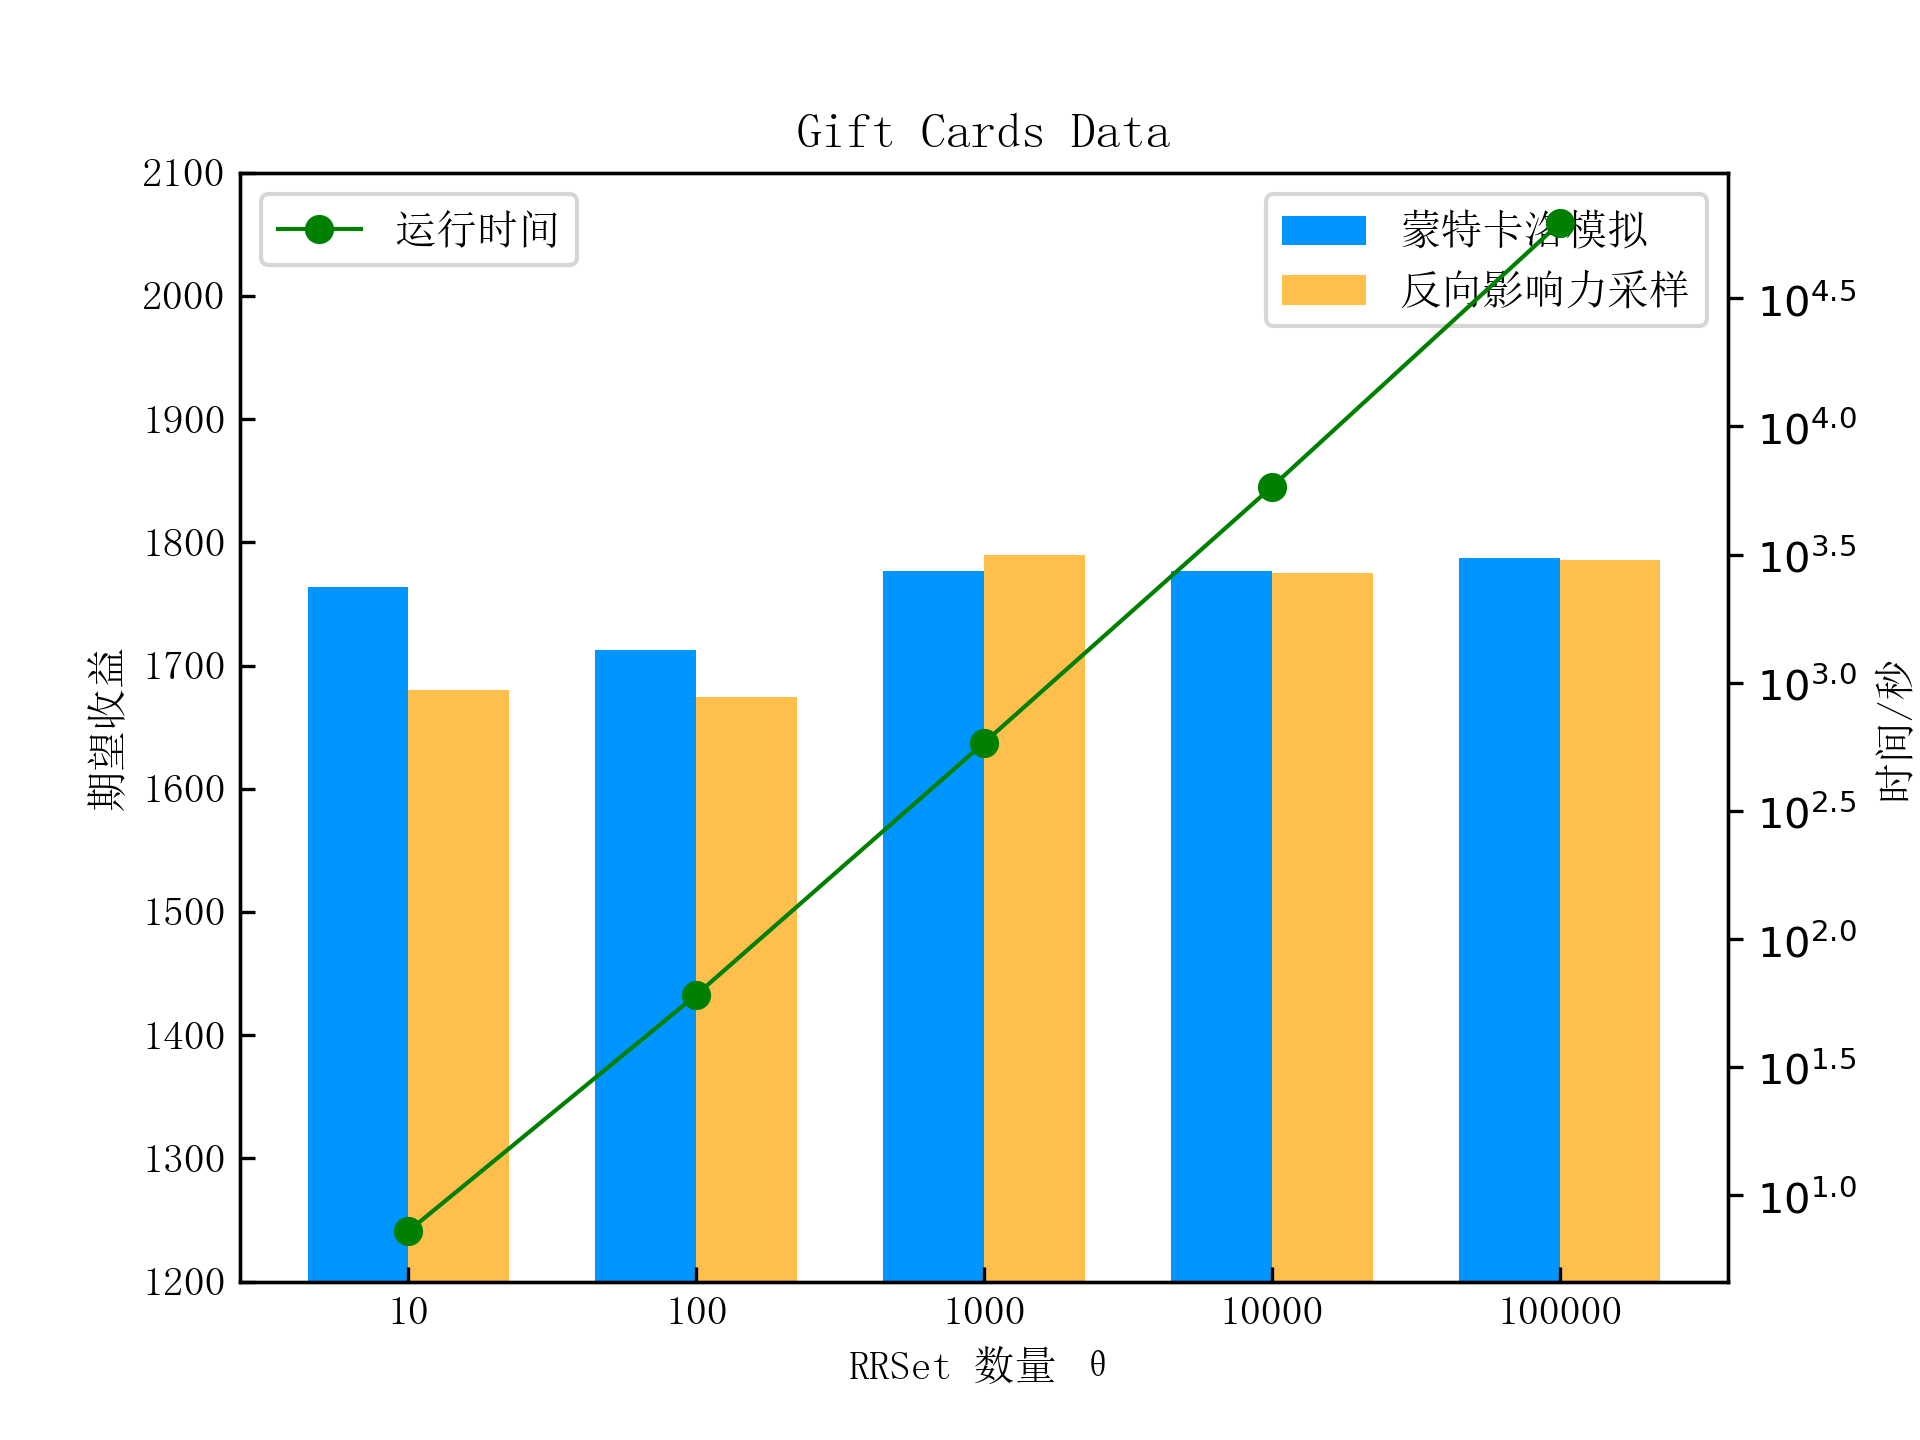
\includegraphics[width=\linewidth]{figure/sasim/theta/cn_gift}
        \caption{Gift Cards数据上$\theta$-期望收益}
        \label{fig:thetasub1}
    \end{subfigure}
    \hfill
    \begin{subfigure}{0.45\textwidth}
        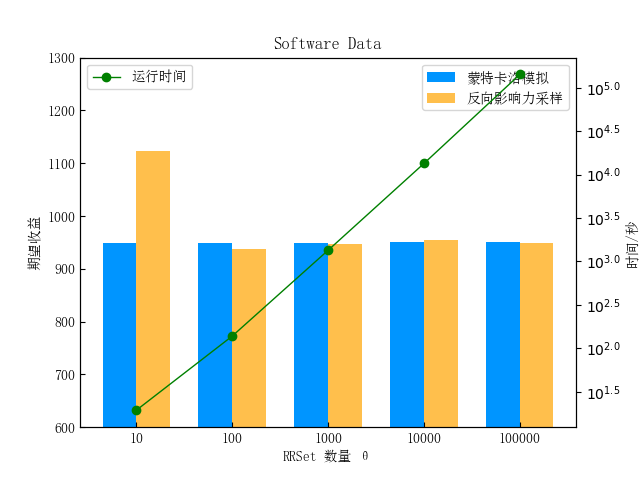
\includegraphics[width=\linewidth]{figure/sasim/theta/cn_software}
        \caption{Software数据上$\theta$-期望收益}
        \label{fig:thetasub2}
    \end{subfigure}

    \medskip

    \begin{subfigure}{0.45\textwidth}
       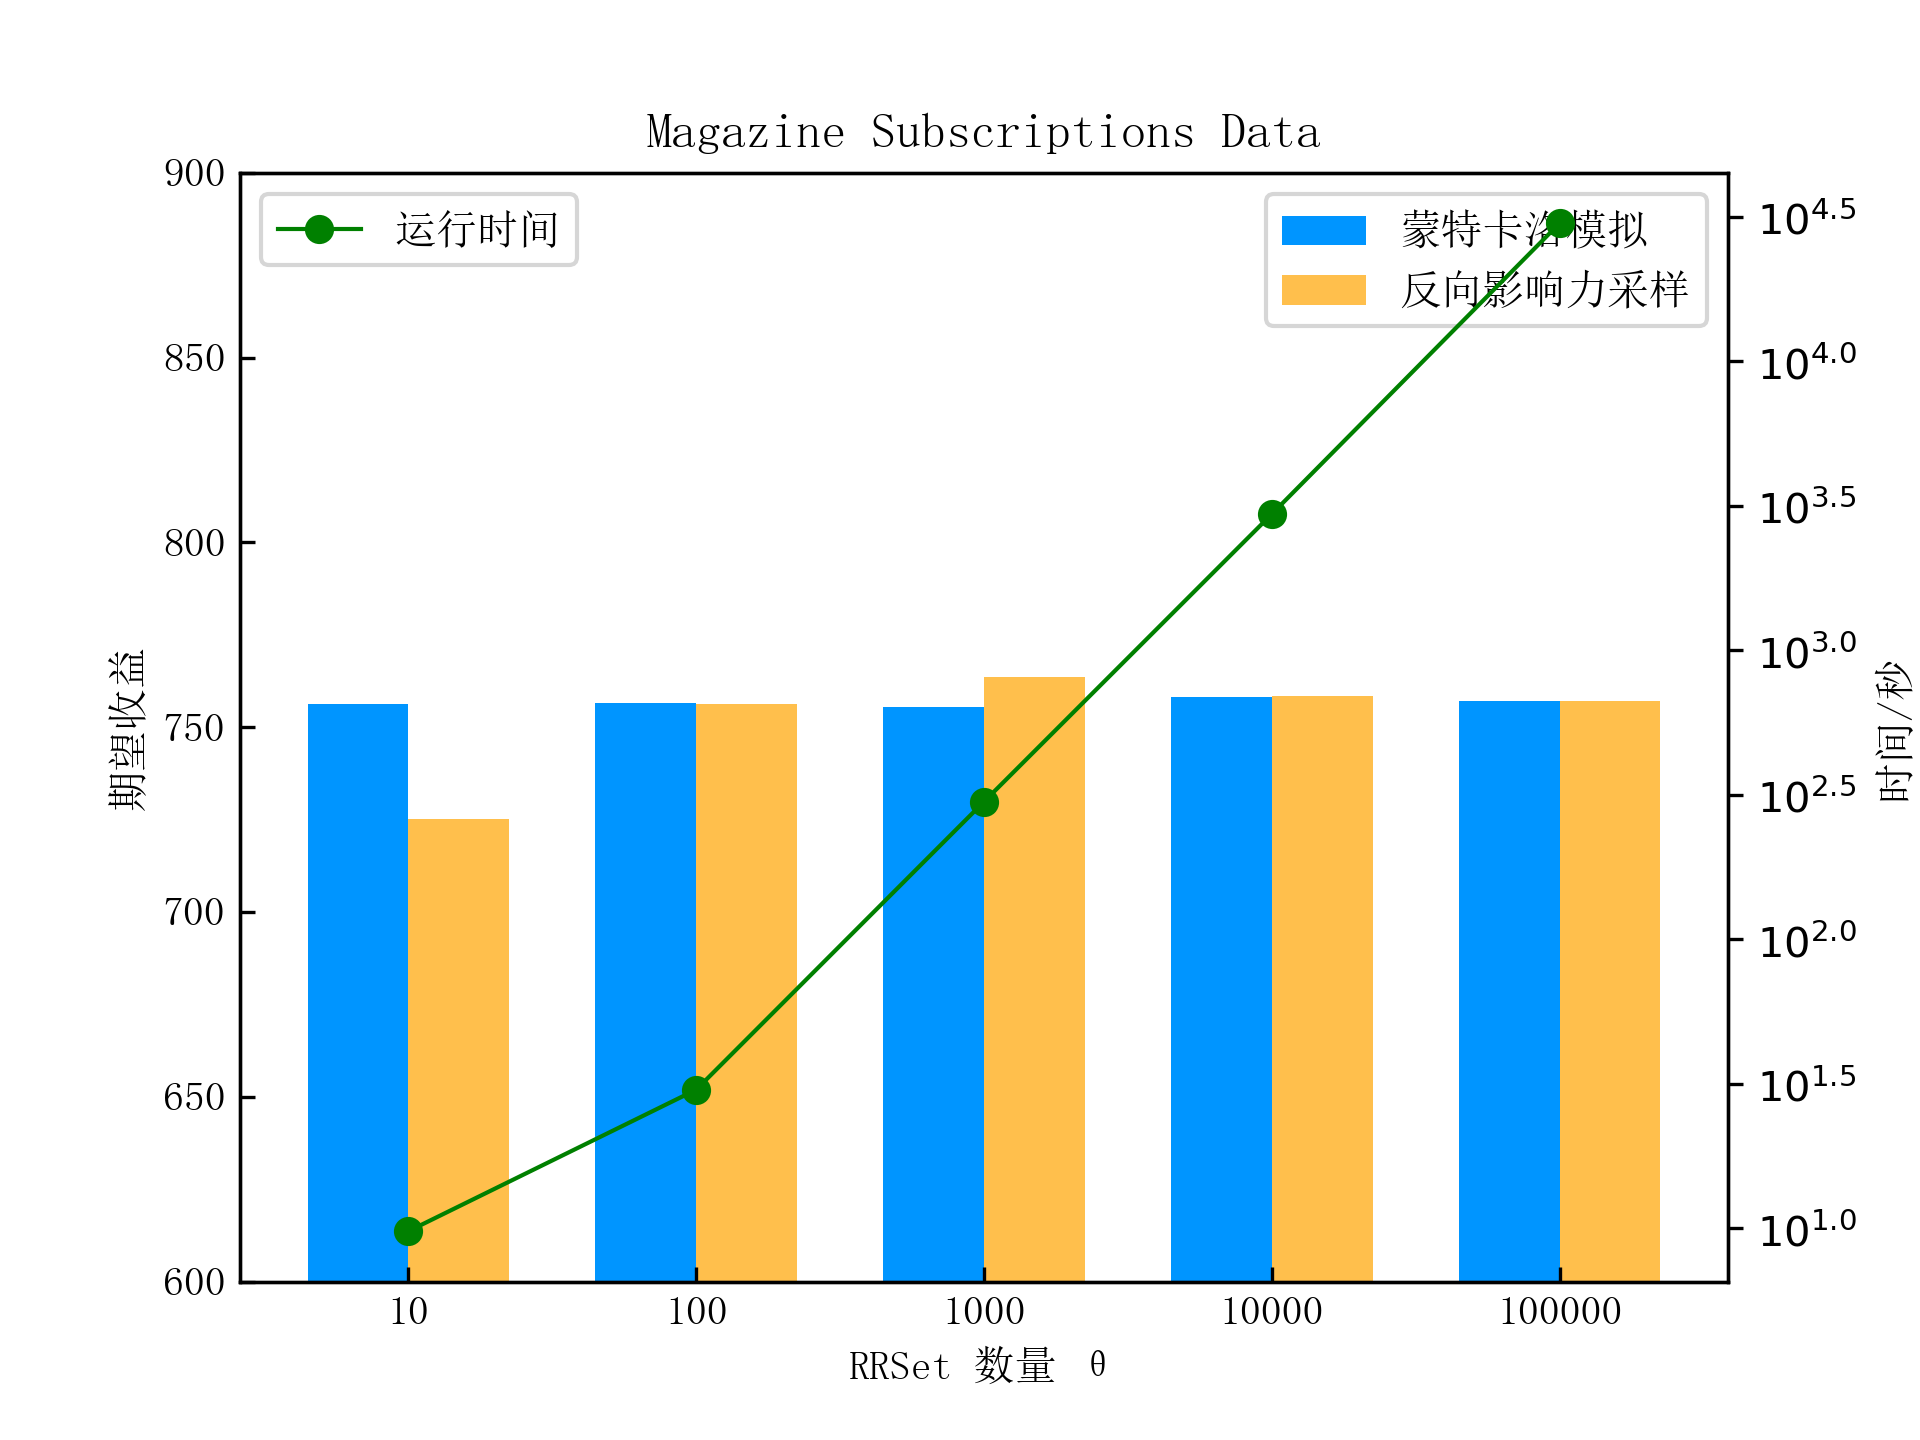
\includegraphics[width=\linewidth]{figure/sasim/theta/cn_magazine}
        \caption{Magazine Subscriptions数据上$\theta$-期望收益}
        \label{fig:thetasub3}
    \end{subfigure}
    \hfill
    \begin{subfigure}{0.45\textwidth}
        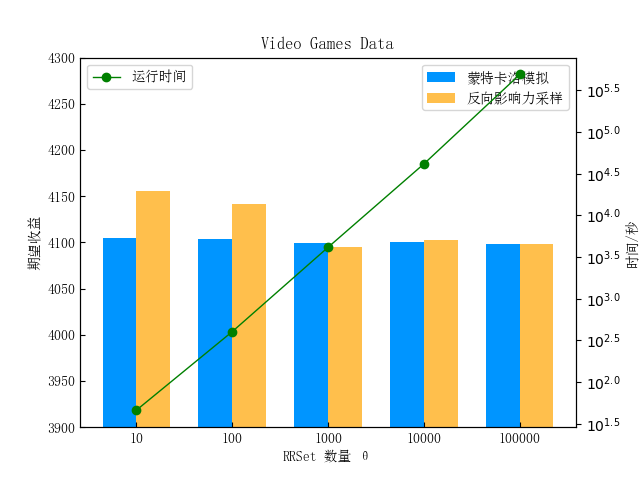
\includegraphics[width=\linewidth]{figure/sasim/theta/cn_video}
        \caption{Video Games数据上$\theta$-期望收益}
        \label{fig:thetasub4}
    \end{subfigure}

    \caption{多轮广告序列推荐实验 $\theta$-期望收益}
    \label{fig:theta}
\end{figure}

如图\ref{fig:theta}所示,随着$\theta$的增大,两种最终得到的期望收益的变化并不明显,说明即使是较小的$\theta$,也能得出比较好的效果。但$\theta$过小时,多轮反向采样的结果与蒙特卡洛模拟结果可能相差较大, 达到$1000$以上后,两者基本持平,并且观察推荐的广告序列结果,基本没有发生变化,结果数据波动较小。而算法的运行时间会随着$\theta$的增大线性增长。因此在下面的实验中,为了兼顾算法的效果、稳定性和运行效率,使用了$\theta=1000$作为反向采样次数。在实际应用中,也可以根据需求牺牲部分置信度缩小$\theta$的大小来满足效率要求。

\subsection{对比实验结果}

考虑用户网络传播的影响、广告边的关联、多轮传播等因素,选择以下共7种方法进行对比:

\begin{itemize}
    \item {\bfseries 边贪心}:本文提出的多轮社交广告序列影响最大化解决方案。基于广告边的贪心,使用多轮反向影响力采样估计边际期望收益,并使用三明治方法取三个结果中最好的序列作为最终结果。
    \item {\bfseries 点贪心}:只考虑广告网络中自环的收益,不考虑广告之间的促进作用。使用多轮反向影响力采样估计点的边际期望收益。将影响力最大化领域中经典的贪心方法\cite{kempe2003maximizing}应用于广告网络中,作为广告节点的选择方法。
    \item {\bfseries 动态规划}:对Tang\cite{tang2018social}提出的算法微调,假设用户看完一个广告会继续浏览的概率为1,由多轮反向影响力采样方法提供广告收益部分的估计。该算法会先将所有广告节点按照期望收益排序,然后使用动态规划选择广告序列。并且每一轮推荐重新运行该算法以适应多轮框架。
    \item {\bfseries 随机选择}:平凡算法,随机选择广告推荐。
    \item {\bfseries 边贪心(无传播)}:去除边贪心算法中多轮反向影响力采样部分,不考虑用户网络的信息传播。
    \item {\bfseries 点贪心(无传播)}:去除点贪心算法中多轮反向影响力采样部分,不考虑用户网络的信息传播。
    \item {\bfseries 每轮相同}:第一轮使用边贪心算法选取广告序列,后续每一轮推荐与对一轮相同的广告序列。 
\end{itemize}

\begin{figure}[th]
    \centering
    \begin{subfigure}{0.45\textwidth}
        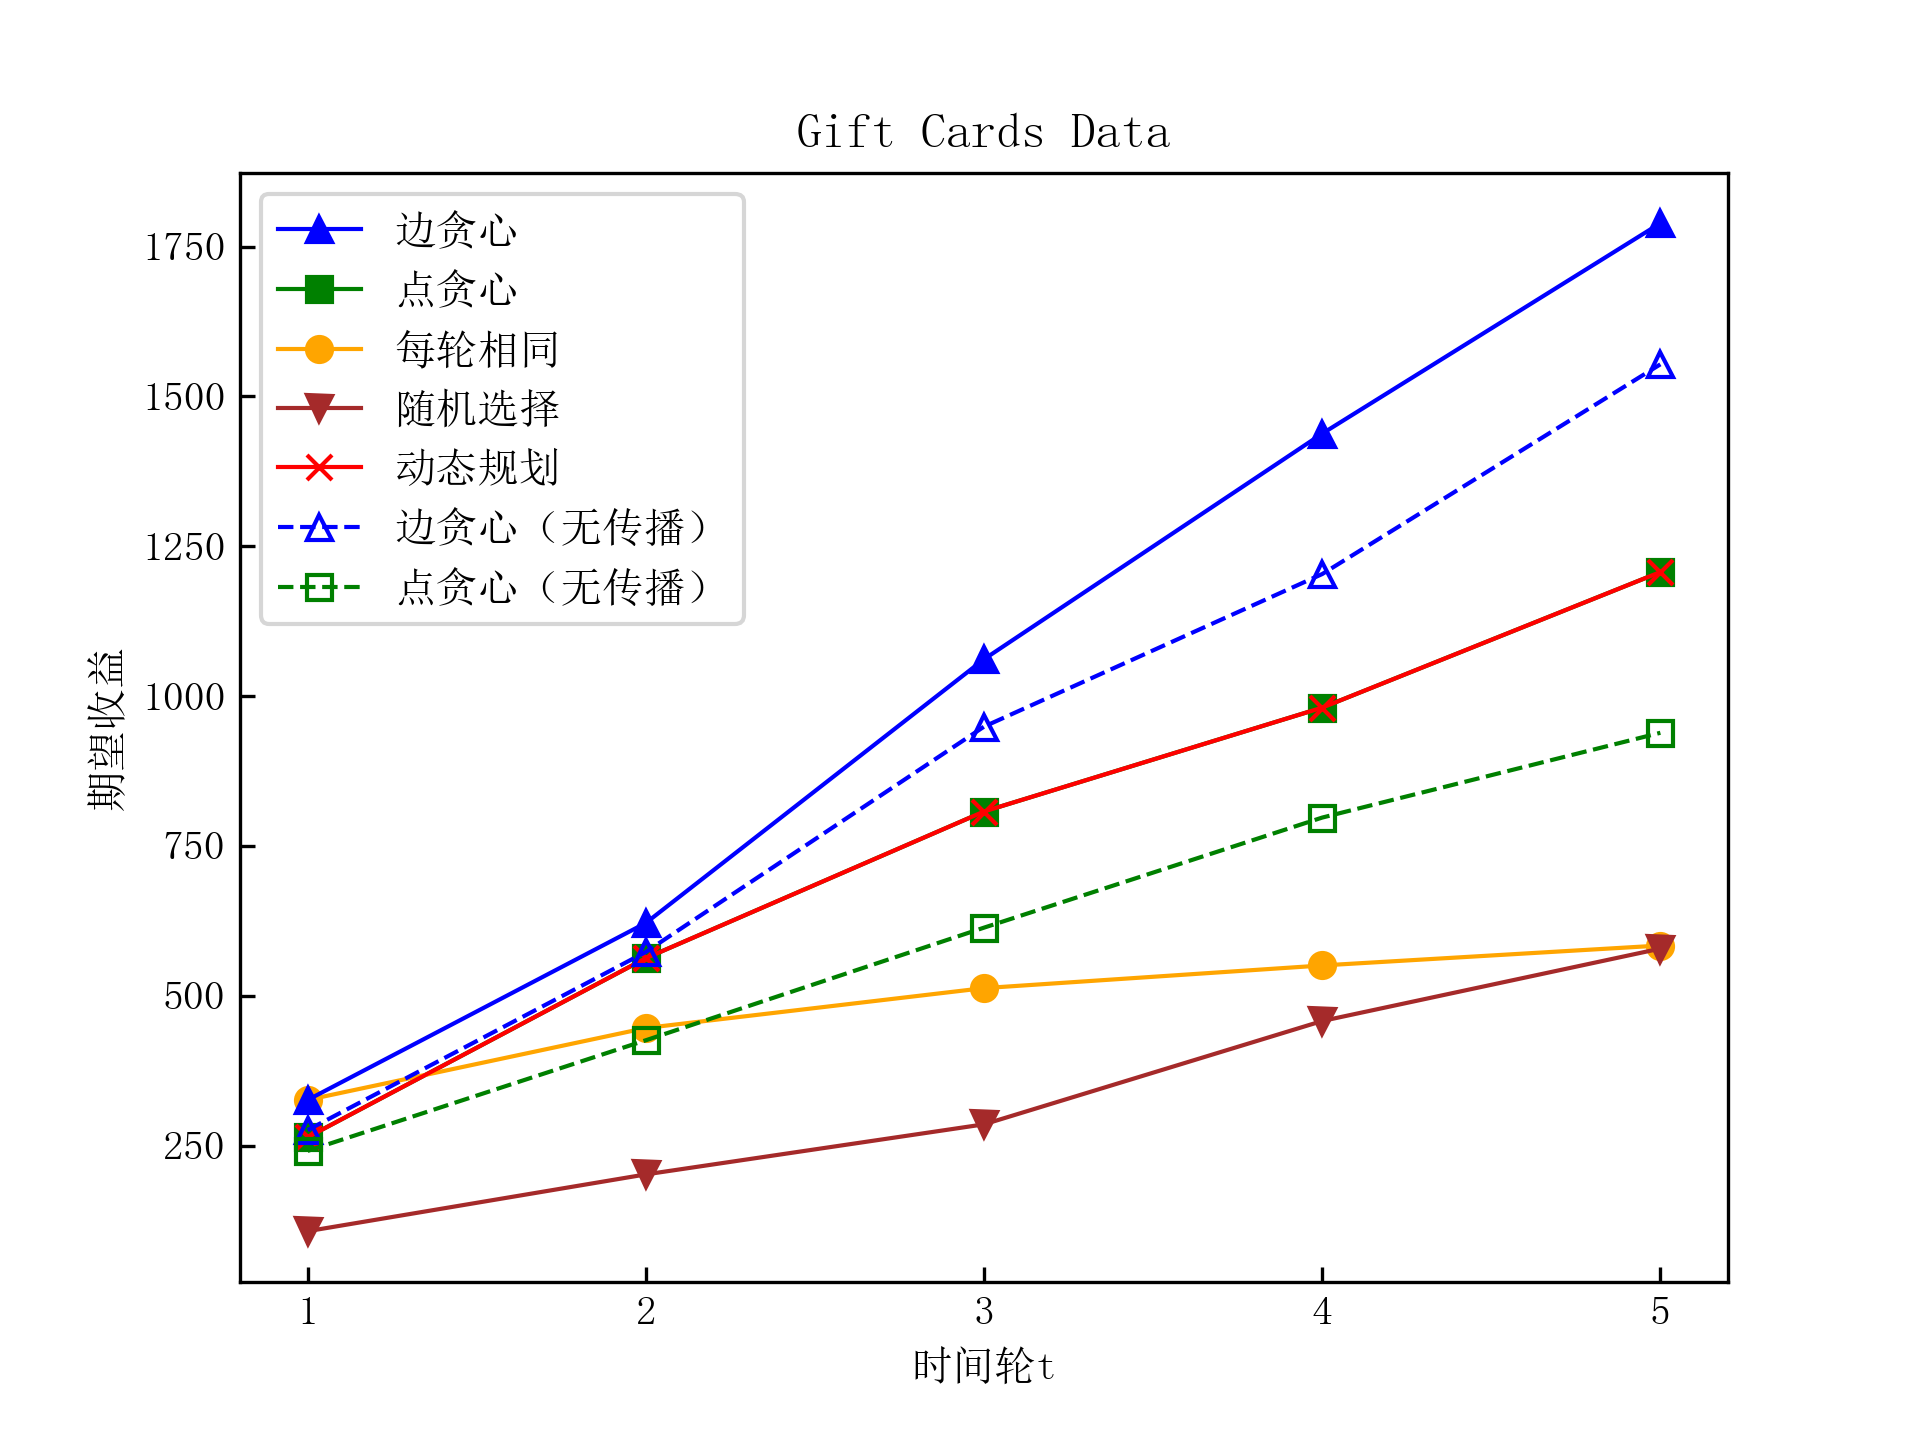
\includegraphics[width=\linewidth]{figure/sasim/nonadp/non_cn_gift}
        \caption{Gift Cards数据上$t$-期望收益}
        \label{fig:non1}
    \end{subfigure}
    \hfill
    \begin{subfigure}{0.45\textwidth}
        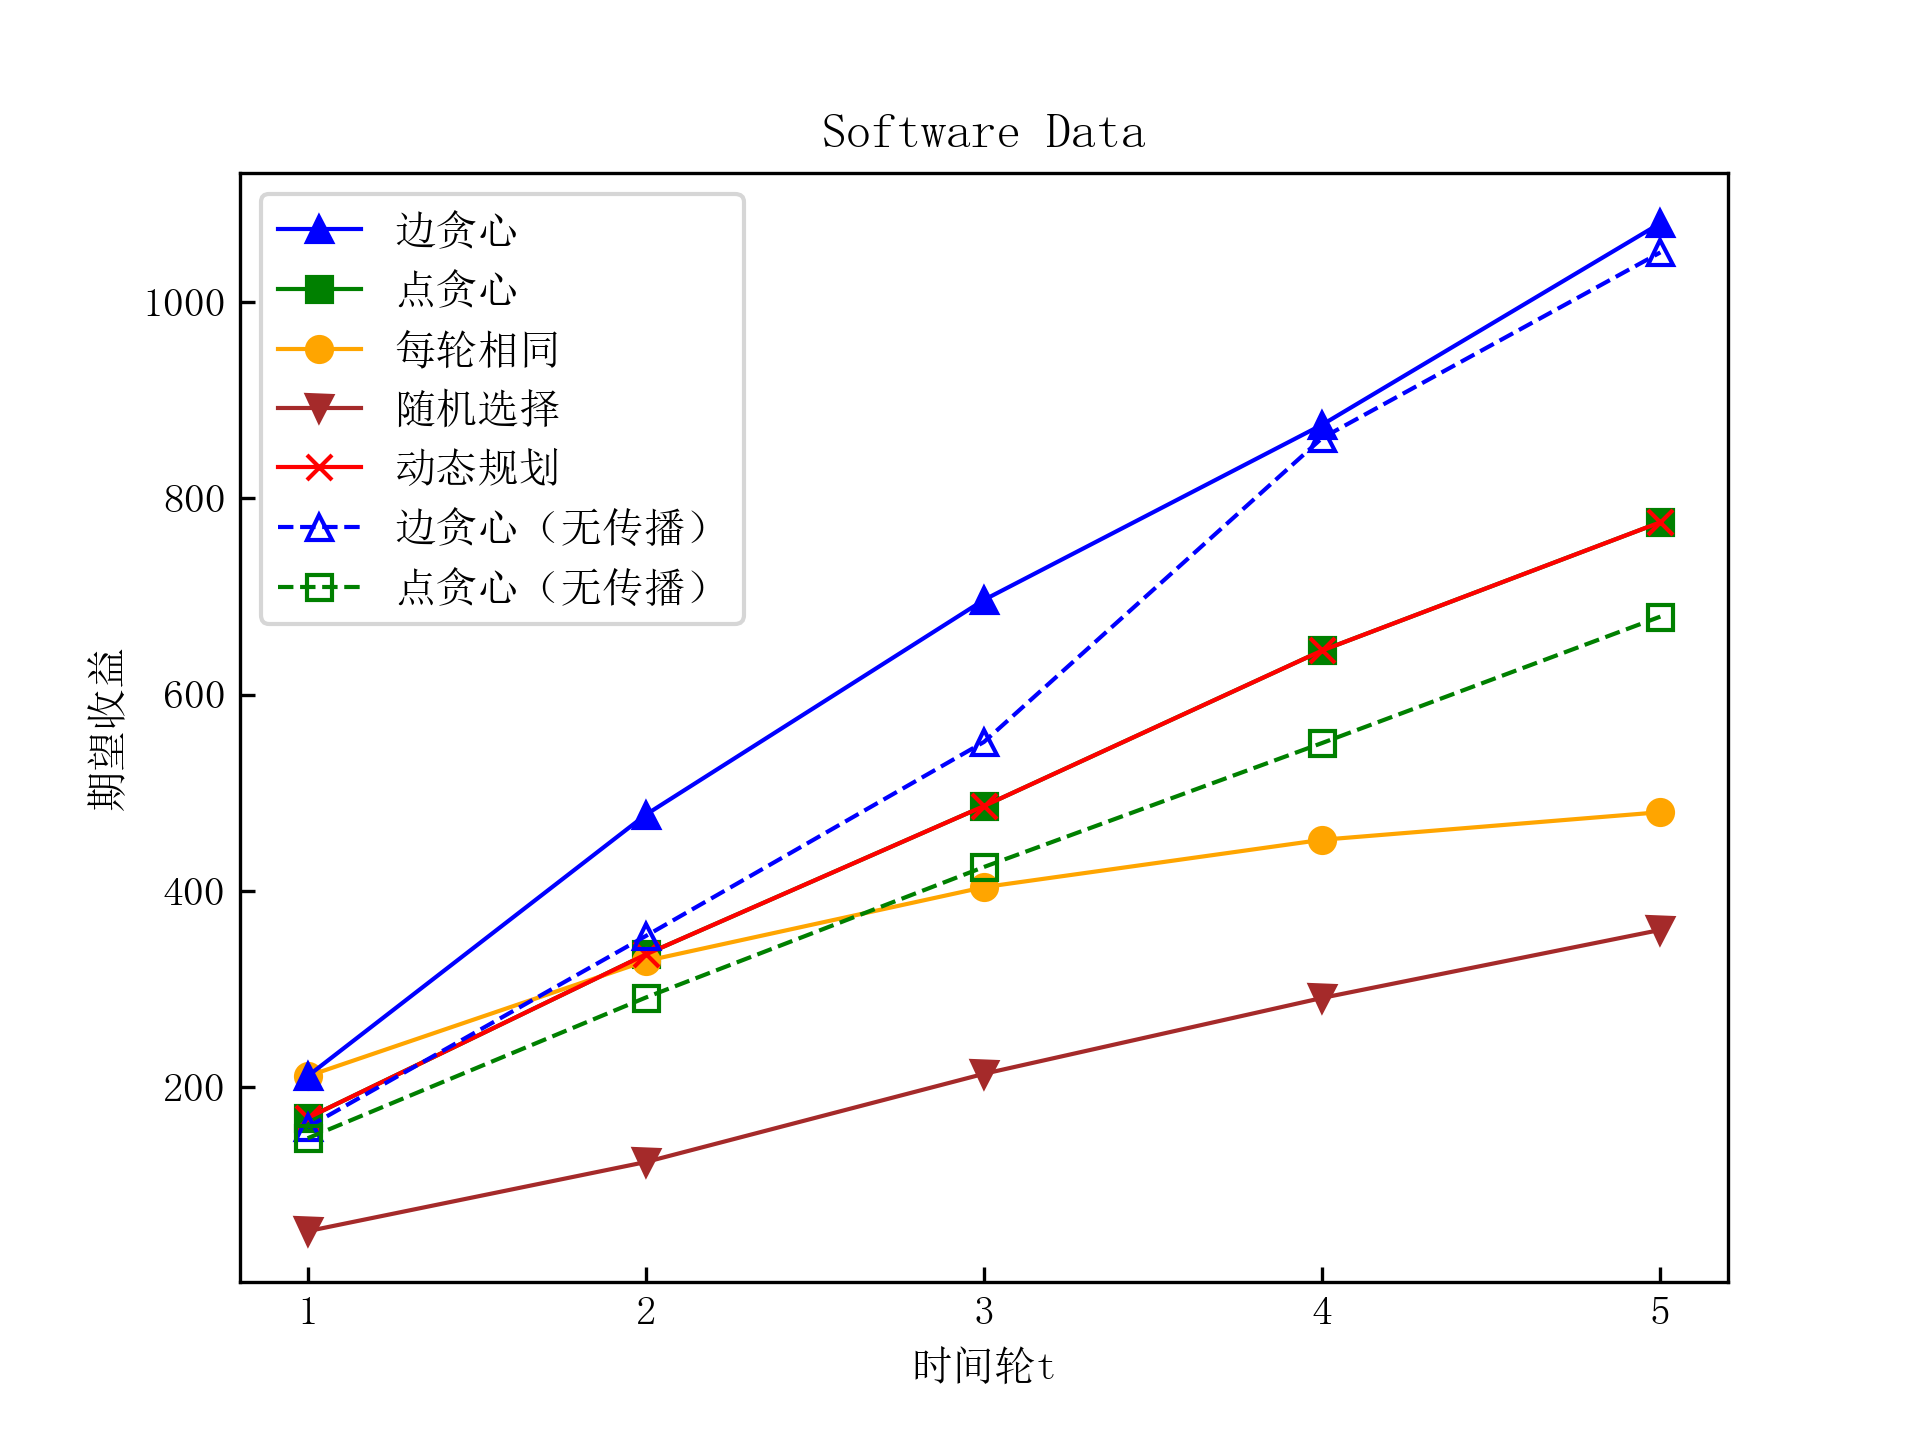
\includegraphics[width=\linewidth]{figure/sasim/nonadp/non_cn_software}
        \caption{Software数据上$t$-期望收益}
        \label{fig:non2}
    \end{subfigure}

    \medskip

    \begin{subfigure}{0.45\textwidth}
       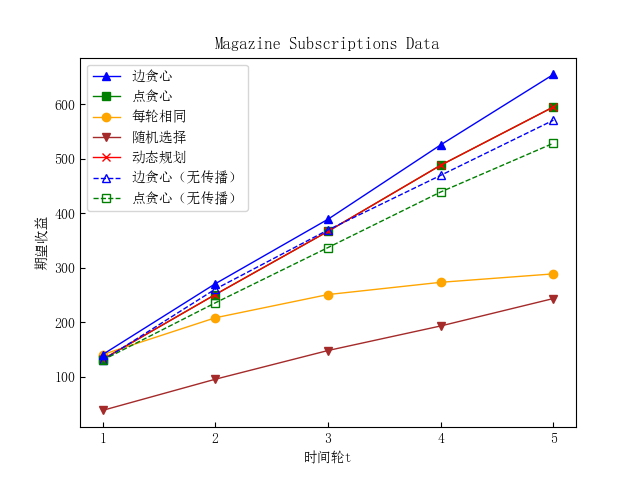
\includegraphics[width=\linewidth]{figure/sasim/nonadp/non_cn_magazine}
        \caption{Magazine Subscriptions数据上$t$-期望收益}
        \label{fig:non3}
    \end{subfigure}
    \hfill
    \begin{subfigure}{0.45\textwidth}
        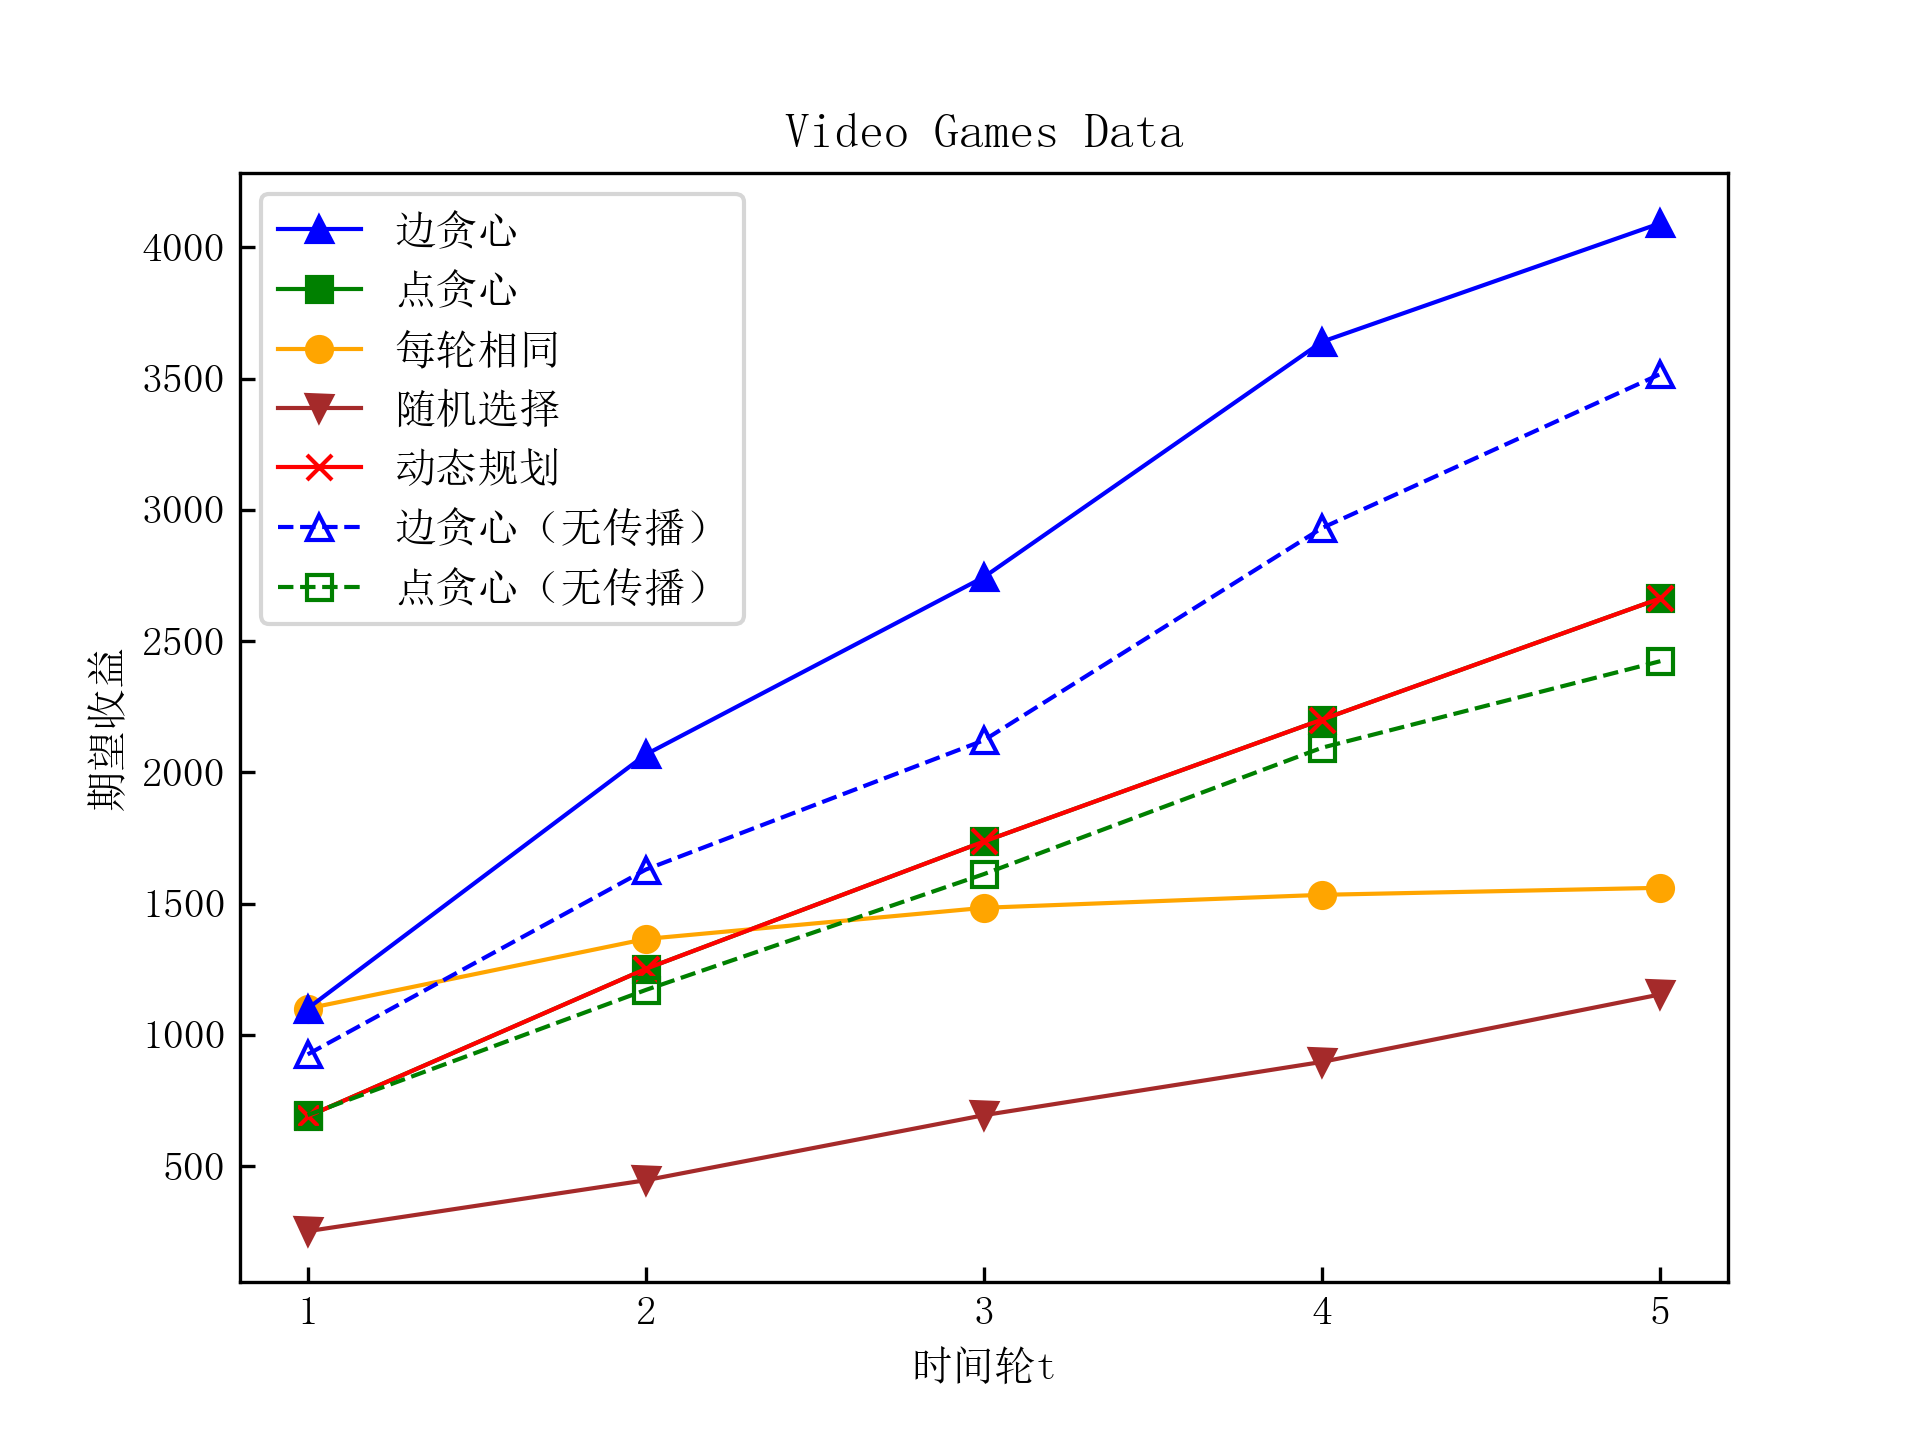
\includegraphics[width=\linewidth]{figure/sasim/nonadp/non_cn_video}
        \caption{Video Games数据上$t$-期望收益}
        \label{fig:non4}
    \end{subfigure}
    \caption{多轮广告序列推荐实验 $t$-期望收益}
    \label{fig:non}
\end{figure}

如图\ref{fig:non}所示,边贪心算法在不同大小的数据集上都优于其他算法。并且相较于平凡的随机选择算法,即使是每轮推荐相同的广告序列也有明显优势,说明边贪心第一轮选择的广告序列较为优秀。但每轮相同和随机选择方法在轮数较大时都明显不如其他算法,其他算法会随着轮数增加更新已推荐广告的收益,更加合理地进行选择。

点贪心算法和动态规划算法基本重合,是因为广告节点之间的收益相对独立,在没有推荐重复广告的情况下,贪心和动态规划的结果基本一致,而重复推荐广告的收益大多较低。两者都没有考虑广告边对结果的影响,因此在广告网络较为稠密的三个数据集上边贪心算法明显更优,期望收益高出至少40\%。而在广告网络较为稀疏的Magazine Subscriptions数据集上,与边贪心算法的效果比较接近,边贪心算法只领先10\%。广告网络稀疏时,广告之间的联系较弱,广告节点的权重相对提升。这也说明边贪心算法在稠密广告网络上更加适用。但结合了三明治方法的边贪心算法会综合考虑广告之间的联系和广告本身的权重,并且三明治方法的下界函数也相当于进行了点贪心,所以即使在广告网络稀疏的情况下也至少不会差于点贪心算法。

图\ref{fig:non}中的两条虚线展示了不考虑用户网络影响力传播的情况。类似地,在用户网络较为稠密的三个数据集上,无传播的算法都表现较差。而在用户网络较为稀疏的Software数据集上,无传播的边贪心算法与有传播的边贪心算法效果较为接近。无传播的算法不考虑传播结果,就无法区分影响力大的用户和影响力小的用户,可能部分用户虽然对广告序列的接收程度很高,但无法造成大量影响导致最终结果较差。在用户网络稀疏的图上,用户的影响力差距较小,会降低影响力传播对结果的贡献,但无法完全消除。有传播的算法还是优于无传播的算法。用户网络越复杂,用户之间的影响力区别越大,有传播的算法越有优势。

\begin{figure}[th]
    \centering
    \begin{subfigure}{0.45\textwidth}
        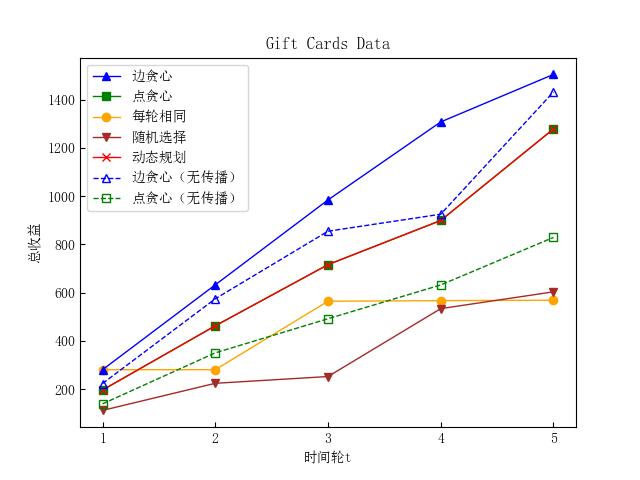
\includegraphics[width=\linewidth]{figure/sasim/adp/adp_cn_gift}
        \caption{Gift Cards数据上动态$t$-期望收益}
        \label{fig:adp1}
    \end{subfigure}
    \hfill
    \begin{subfigure}{0.45\textwidth}
        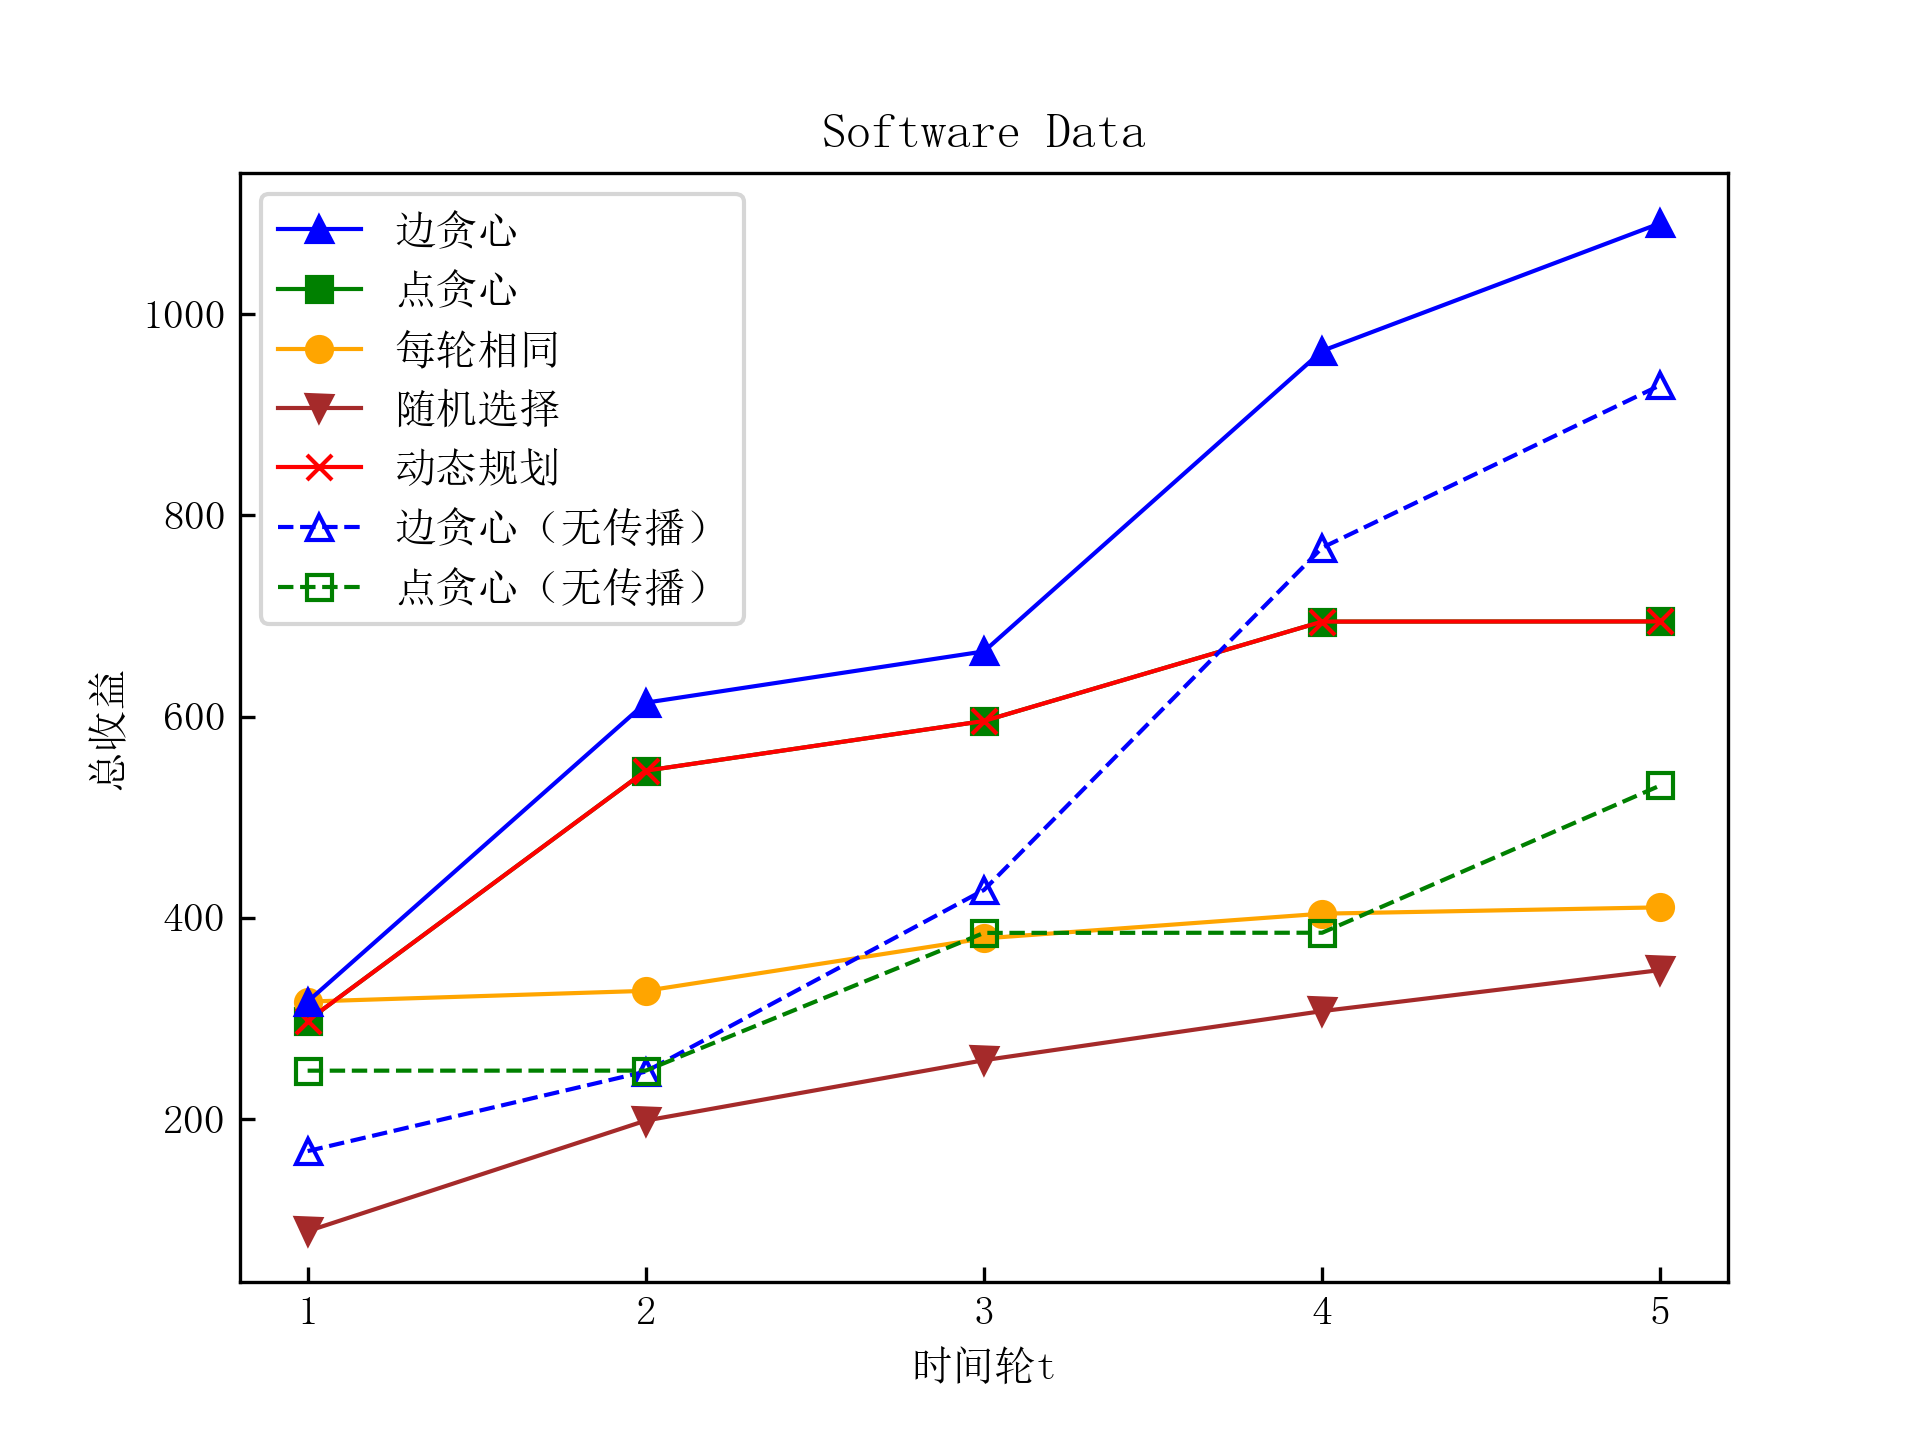
\includegraphics[width=\linewidth]{figure/sasim/adp/adp_cn_software}
        \caption{Software数据上动态$t$-期望收益}
        \label{fig:adp2}
    \end{subfigure}

    \medskip

    \begin{subfigure}{0.45\textwidth}
       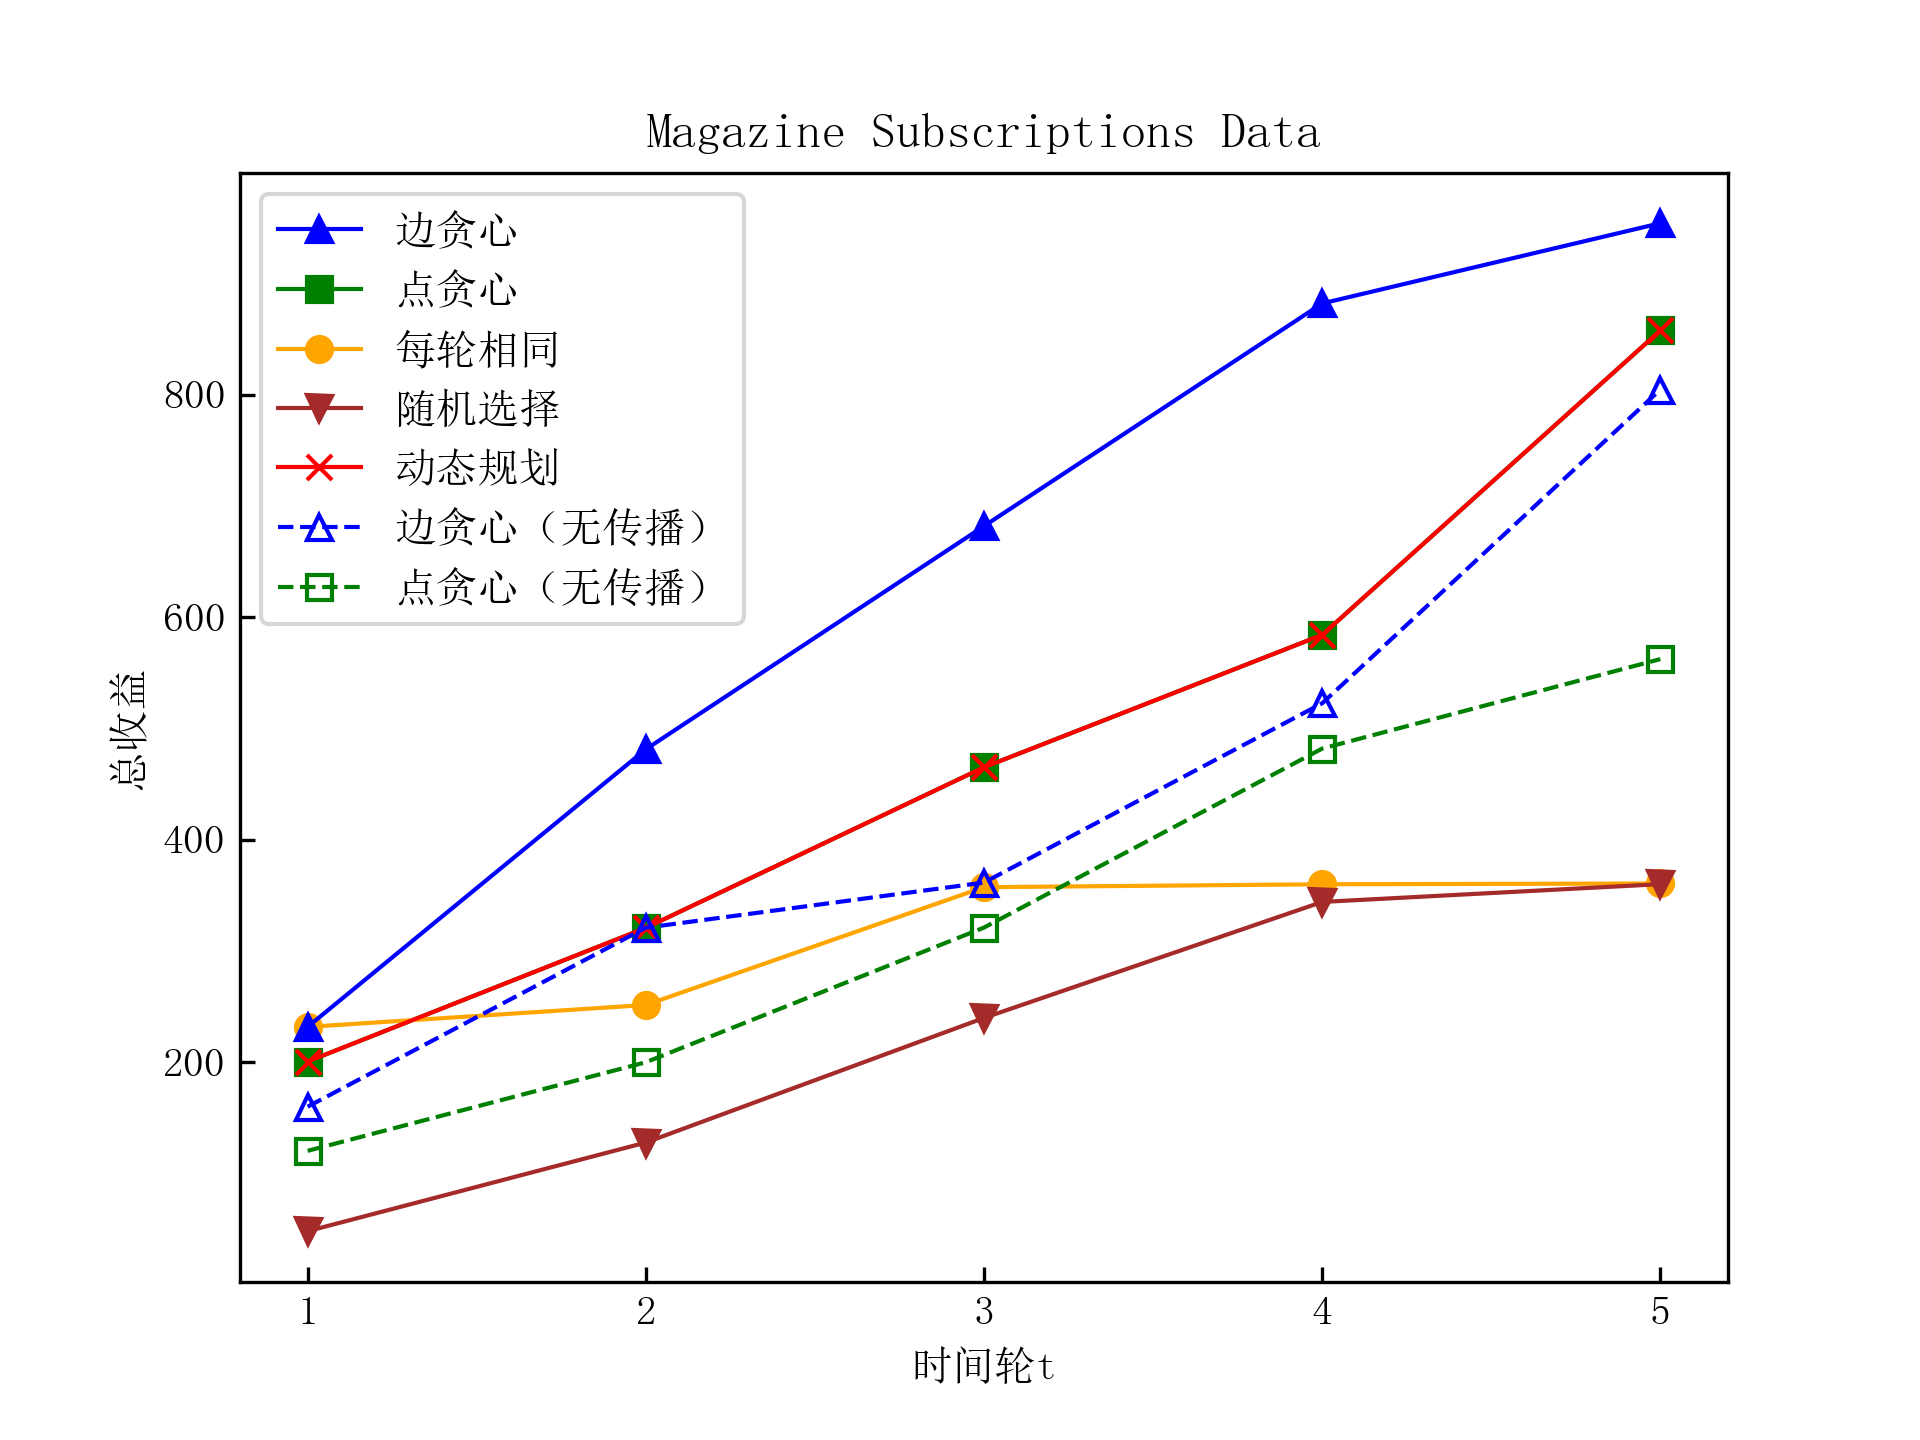
\includegraphics[width=\linewidth]{figure/sasim/adp/adp_cn_magazine}
        \caption{Magazine Subscriptions数据上动态$t$-期望收益}
        \label{fig:adp3}
    \end{subfigure}
    \hfill
    \begin{subfigure}{0.45\textwidth}
        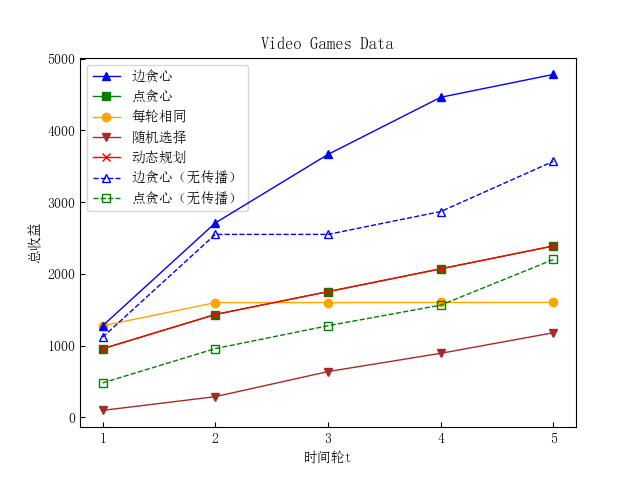
\includegraphics[width=\linewidth]{figure/sasim/adp/adp_cn_video}
        \caption{Video Games数据上动态$t$-期望收益}
        \label{fig:adp4}
    \end{subfigure}
    \caption{动态轮广告序列影响最大化实验 $t$-期望收益}
    \label{fig:adp}
\end{figure}

如图\ref{fig:adp}所示,动态结果与非动态的结果趋势大致相同。我们提出的动态边贪心算法在不同数据集上都展现了优势。动态场景下不同的是,每一轮推荐结束后用户都会对推荐的广告随机地做出确定性的选择,实际的观测结果可能会与期望值有较大的差距,因此在动态实验中的结果线条相比于静态结果的线条要更加曲折。但好在算法可以观察到这一结果,在下一轮的多轮反向影响力采样过程中,会将这些已确定的值修正,使得算法能在当前情况下选择期望收益最大的序列进行下一轮推荐,使整体的推荐收益得到保证。

综上所述,对比实验证明了边贪心算法的有效性:能够有效地综合利用用户对广告的接受程度、广告之间的关联、用户网络的影响力传播等信息推荐多轮广告序列,在非动态和动态两种场景下,算法在几个的Amazon评论数据集上效果均较已有算法有明显优势。

\subsection{效率实验}

多轮社交广告序列影响最大化算法的计算时间主要用于评估广告序列的收益,即使用多轮反向影响力采样的部分。我们首次将用户网络和广告网络同时纳入多轮广告推荐模型中,这使得其他对比算法在估算广告序列的期望收益时,只能依赖于我们提出的多轮反向影响力采样方法。在动态观测的情况下,也可以通过修改已观测到的用户的反向影响力采样值来快速估算收益。为了体现多轮反向影响力对算法效率的提升,我们在评估广告序列收益这一点上与应用于影响力最大化问题中的蒙特卡洛模拟方法\cite{kempe2003maximizing}进行了对比。

我们分别使用多轮反向影响力采样方法(mRIS)和蒙特卡洛模拟方法(MC)对边贪心输出的多轮广告序列进行价值评估,采样次数和蒙特卡洛模拟次数均设为$\theta={10,100,1000,10000,100000}$次。四个数据集上的评估结果和运行时间如表\ref{tab:gif},\ref{tab:sof},\ref{tab:mag}和\ref{tab:vid}所示。模拟次数越多,得到的值越趋于收敛,我们将$\theta=100000$时的MC估计值结果作为一个比较的标准值。观察到,在同等采样次数和模拟次数的情况下,mRIS的估计值和MC估计值的准确度基本相当。然而,mRIS的运行速度明显快于MC。mRIS需要先生成多轮反向可达集采样,然后再进行评估计算,两者加起来的时间为评估的总耗时。MC评估的用时基本上是mRIS生成时间的100倍,是mRIS评估时间的1000倍。因此,使用mRIS进行评估至少能比传统方法提升效率100倍,而且,在算法过程中,需要进行相当多次的评估。如果使用mRIS方法,多轮反向可达集是可以反复使用的,只需生成一次,每次评估只需花费评估时间。而MC方法每次都需要进行完整的模拟。

\begin{table}[ht]
    \centering
    \caption{Gift Cards数据上序列价值评估和运行时间对比\label{tab:gif}}
    \begin{tabular}{|c|c|c|c|c|c|}
        \hline
         & $\theta=10$ & $\theta=100$ & $\theta=1000$ & $\theta=10000$ & $\theta=100000$ \\
        \hline
        \text{mRIS 估计值} & 1656.6 & 1756.9 & 1765.4 & 1771.8 & 1776.6 \\
        \hline
        \text{MC 估计值} & 1795.3 & 1773.3 & 1768.2 & 1776.7 & 1780.1 \\
        \hline
        \text{mRIS 生成时间/s} & 0.0462 & 0.2980 & 4.4506 & 37.8899 & 376.1852 \\
        \hline
        \text{mRIS 评估时间/s} & 0.0002 & 0.0013 & 0.0101 & 0.0990 & 1.1740 \\
        \hline
        \text{MC 评估时间/s} & 0.2979 & 2.8844 & 26.9915 & 262.8904 & 2593.0679 \\
        \hline
    \end{tabular}
\end{table}


\begin{table}[ht]
    \centering
    \caption{Software数据上序列价值评估和运行时间对比\label{tab:sof}}
    \begin{tabular}{|c|c|c|c|c|c|}
        \hline
        & $\theta=10$ & $\theta=100$ & $\theta=1000$ & $\theta=10000$ & $\theta=100000$ \\
        \hline
        \text{mRIS 估计值} & 863.5 & 1049.9 & 1046.9 & 1092.0 & 1087.6 \\
        \hline
        \text{MC 估计值} & 1127.4 & 1082.0 & 1086.2 & 1089.8 & 1089.2 \\
        \hline
        \text{mRIS 生成时间/s} & 0.0090 & 0.0861 & 0.8156 & 9.5258 & 92.4616 \\
        \hline
        \text{mRIS 评估时间/s} & 0.0003 & 0.0011 & 0.0091 & 0.0956 & 0.9326 \\
        \hline
        \text{MC 评估时间/s} & 0.1088 & 1.0373 & 10.4475 & 105.4092 & 1060.6928 \\
        \hline
    \end{tabular}
\end{table}

\begin{table}[ht]
    \centering
    \caption{Magazine Subscriptions数据上序列价值评估和运行时间对比\label{tab:mag}}
    \begin{tabular}{|c|c|c|c|c|c|}
        \hline
        & $\theta=10$ & $\theta=100$ & $\theta=1000$ & $\theta=10000$ & $\theta=100000$ \\
        \hline
        \text{mRIS 估计值} & 691.3 & 663.7 & 656.1 & 650.4 & 650.0 \\
        \hline
        \text{MC 估计值} & 624.3 & 663.6 & 647.1 & 650.6 & 650.2 \\
        \hline
        \text{mRIS 生成时间/s} & 0.0386 & 0.3546 & 2.8631 & 27.5445 & 281.0090 \\
        \hline
        \text{mRIS 评估时间/s} & 0.0003 & 0.0014 & 0.0133 & 0.1209 & 1.3040 \\
        \hline
        \text{MC 评估时间/s} & 0.2118 & 1.7267 & 17.7301 & 174.1293 & 1691.2034 \\
        \hline
    \end{tabular}
\end{table}


\begin{table}[ht]
    \centering
    \caption{Video Games数据上序列价值评估和运行时间对比\label{tab:vid}}
    \begin{tabular}{|c|c|c|c|c|c|}
        \hline
        & $\theta=10$ & $\theta=100$ & $\theta=1000$ & $\theta=10000$ & $\theta=100000$ \\
        \hline
        \text{mRIS 估计值} & 4155.7 & 4114.1 & 4107.9 & 4097.2 & 4099.3 \\
        \hline
        \text{MC 估计值} & 4265.0 & 4162.2 & 4107.2 & 4091.5 & 4100.7 \\
        \hline
        \text{mRIS 生成时间/s} & 0.2503 & 2.5926 & 24.6597 & 250.6203 & 2416.6024 \\
        \hline
        \text{mRIS 评估时间/s} & 0.0003 & 0.0017 & 0.0137 & 0.1560 & 1.4790 \\
        \hline
        \text{MC 评估时间/s} & 1.5178 & 16.0196 & 158.0936 & 1546.4910 & 14374.9731 \\
        \hline
    \end{tabular}
\end{table}

因此,本文提出的多轮反向影响力采样方法不仅能够大大提升算法的效率,也可以在多轮社交广告序列影响最大化问题上与各种其他已有的算法相结合来产生新的解决方案,为快速估计广告收益提供了一种较为通用的方法。

\section{本章小结}

在本章中,分别介绍了鲁棒序列子模最大化算法实验和多轮社交广告序列影响最大化推荐算法实验。

\ref{sec:5_1}节展示了鲁棒序列子模最大化算法的实验设置和实验结果。分别在Amazon评论数据集和Wikispeedia数据集上进行了广告推荐实验和链路预测实验。采用了准确度得分、序列得分、目标函数值三种评价指标从多角度对实验结果进行评估。通过对比实验结果验证了我们提出的鲁棒序列子模最大化算法的有效性和鲁棒性。

\ref{sec:5_2}节展示了多轮社交广告序列影响最大化推荐算法实验的实验设置和实验结果。实验在Amazon评论数据集上进行,先通过参数实验综合考虑实验效果和时间,选择合适的实验参数。通过在非动态和动态设定下的与不同对比方法的比较验证了多轮社交广告序列影响最大化算法够有效地综合利用用户对广告的接受程度、广告之间的关联、用户网络的影响力传播等信息,体现了在推荐多轮广告序列的场景下的优势。此外,通过效率实验验证了我们提出的多轮反向影响力采样技术能够显著提升算法的效率。

\chapter{总结和展望}

\section{工作总结}

随着移动设备和社交网络的蓬勃发展,人们花在浏览社交平台信息上的时间越来越多,因此,给用户推荐个性化的广告序列成为一个具有挑战性问题。而然而,在当前的广告序列推荐领域中,尚未有研究同时将用户对广告本身的兴趣、广告之间的正向关系、用户选择性接受广告以及用户社交网络影响力传播因素同时纳入考虑。本文将网络子模函数引入到序列广告推荐问题中,加强了广告之间正向关系在算法选择过程中的重要性。

针对用户不接受部分广告的最差情况,本文定义了鲁棒序列网络子模最大化问题,分析了已有的序列贪心算法在移除部分节点情况下的弊端,进一步提出了采用两段式贪心的鲁棒序列网络子模最大化算法。该算法的核心在于,将序列分为两部分,分别做两次独立的贪心选择,在做第二次贪心时完全排除掉第一次贪心的结果。避免序列价值过度集中于序列的前部节点,从而提升广告序列的鲁棒性。本文给出了鲁棒序列网络子模算法在$\tau = 1$和$1 < \tau < k$时的近似比,分析了不同情况下近似比的取值,并证明了其正确性。

结合社交网络影响力传播因素,将影响力最大化问题进一步引入广告序列推荐任务中。本文在广告序列推荐问题上首次将广告网络和用户网络同时纳入模型,在已有的影响力最大化问题和广告推荐问题的基础上,综合用户对广告的偏好、广告之间的促进作用以及用户网络的信息传递,并考虑到广告推荐不是一次性过程,加入多轮推荐的模式,建立能够同时为一组用户服务的多轮广告序列影响力最大化问题模型。多轮社交广告序列影响最大化问题详细定义了目标序列价值函数的计算方法,并给出了基于广告边的贪心框架。本文提出的多轮反向影响力采样方法能够快速估算每条边的边际收益,为边贪心算法的复杂度做出保证。后讨论了目标函数的单调性和子模性,由于目标函数对于边集不满足子模性,引入了三明治方法,通过找到两个满足子模性的上下界函数对原函数夹逼,保证了算法的近似比。此外,在部分实际场景中,可以观测用户对广告的接受情况和在用户网络中的传播结果,针对这种情景,本文拓展了复杂度和近似比与非动态版本相同的动态多轮社交广告序列影响最大化算法。

最后,我们在真实数据集上进行了对比实验,以验证所提出算法的有效性和优越性。鲁棒序列子模最大化算法的评估分别在广告推荐和链路预测两个任务上进行。实验结果显示,该算法在准确度得分、序列得分和目标函数值三种关键评价指标上均优于其他对比算法。这不仅验证了算法所生成序列的有效性,更突出展示了其优秀的鲁棒性表现。

对于多轮社交广告序列影响最大化推荐算法,我们在Amazon评论数据集上进行了多轮广告序列推荐实验。首先通过参数实验确定了合适的实验参数配置。然后在非动态和动态两种设定下进行对比实验。实验结果证明了该算法能够有效地综合利用多方面信息,包括用户对广告的接受程度、广告之间的关联性以及用户网络中的影响力传播等。体现了本文提出的算法在多轮广告序列推荐场景下的独特优势。值得注意的是,由于本文首次使用了同时考虑广告网络和用户网络的模型,因此对比方法中计算序列收益的部分也需要依赖于本文提出的多轮反向影响力采样方法,也证明了本文提出的多轮反向影响力采样方法可以作为一种通用的序列价值快速估算方法,与其他方法结合共同解决多轮社交广告序列影响最大化问题。

综上所述,我们提出的棒序列子模最大化算法和多轮社交广告序列影响最大化推荐算法为广告推荐领域带来了新的解决方案,通过实验验证了其有效性,为实际应用提供了的新工具。

\section{未来展望}

在鲁棒序列网络子模最大化算法的分析和实验中,我们发现序列贪心的局限性在于后续序列的选择和序列价值都围绕着部分核心节点。本文采用了两次独立的贪心方法来削弱这种情况,增强序列的稳定性。在$\tau=0$的部分实验中,发现这种两段式贪心即使在不移除元素的情况下,也有可能优于一次贪心的算法。这说明直接实施贪心选择有时可能会远离最优解,反而增加独立贪心选择的次数可能才是更优的方向,因此探索如何通过增加独立贪心选择的次数,得到价值和鲁棒性更佳的序列是一个有趣的未来探索方向。

本文提出的多轮社交广告序列影响最大化推荐算法的复杂度瓶颈主要在于多轮反向影响力可达集的个数和广告网络的规模。每次选择了新的边加入集合之后,需要重新计算其他边的边际收益。实际上,因为这条新边而收益发生的变化的边应该是较少的,因此在这部分存在着大量的冗余计算。考虑通过启发式方法规避掉部分重复的计算,提高算法效率也是一个可行的方向。